\documentclass{report}
\usepackage{amsfonts,amsthm,amsmath,latexsym,amssymb}
\usepackage[margin=1.5in]{geometry}
\usepackage{complexity}
\usepackage{graphicx}
\usepackage[titles,subfigure]{tocloft}
\usepackage{scribe-book}
\usepackage[lined,boxed]{algorithm2e}


\usepackage{caption}
\usepackage{subcaption}
\usepackage{float}

\newcommand{\CYCLE}{{\sf CYCLE~}}
\newcommand{\FPSPACE}{{\sf FPSPACE~}}
\newcommand{\N}{{\mathbb{N}}}
\newcommand{\Z}{{\mathbb{Z}}}
\newcommand{\F}{{\mathbb{F}}}

%% For xy matrix
\input xy
\xyoption{all}
\CompileMatrices

\usepackage{tikz}
\usetikzlibrary{arrows}

\usetikzlibrary{calc,through,backgrounds,decorations.pathmorphing}

% Shows lecture titles and sections. Set 0 to list only chapters.
\setcounter{tocdepth}{1}

\begin{document}
\newpage
\setcounter{page}{1}
\pagenumbering{roman}  % Roman numbering in intro portion.
\begin{center}
{\bf \Huge Preface}         
\end{center}

\noindent
Matter to be entered here.

\newpage
\listofscribe          % For automatic scribe list generation.

\newpage
\tableofcontents

\setcounter{page}{1}
\pagenumbering{arabic}  % Arabic page numbering for lectures.

% Autogenerated using Makefile. DO NOT EDIT
\newpage \Lecture{Dinesh K.}{Jan 10, 2012}{4}{Quest for Structure in Counting Problems}
%\theme{Between $\P$ and $\PSPACE$.}
%\lectureplan{Counting problems and their structural complexity. Various attempts to develop the theory and the class $\#\P$. Basic containments.}

%We have seen several decision problems where we are interested in knowing the
%existence or non-existence of objects satisfying a certain property. An
%equally interesting question would be to ask the count of such objects. Such
%problems are called as counting problem.

In the previous lecture, we saw that the counting problem can be as hard as (or 
harder than) the decision problem as given an algorithm for counting problem
the decision problem reduces to just checking the count to be zero or not. We
also saw an easy decision problem \CYCLE whose counting version \#\CYCLE is
\NP-hard (by reduction from {\sf HAMCYCLE}) implying that easy decision
problems can also have corresponding counting problems hard. We also argued
that talking about counting problems still makes sense as the count value,
though exponential, can still be represented in polynomial number of
bits.

In this lecture, we will study counting problems and understand their
structural complexity. We shall also make attempts to develop the theory of
complexity classes capturing the counting problems (especially \#\P). We shall
also discuss their basic containments.

\section{Preliminaries}
Firstly, we fix our computation model where we have a Turing machine with an
input tape, work tape and an output tape. We are interested in the resources
used by the Turing machine - space (considering only the work tape) and time.

We want to capture the notion of counting formally. One such way is to see it
as computing a function $f : \Sigma^* \to \N$ where $\Sigma=\{0,1\}$ which
gives an integer value. So, how can we capture the notion of computing a
function? There are two possible ways of capturing function computation.
\begin{description}
\item[Variant 1] We say that a function $f$ is computable if each bit of the
output can be computed in some decision complexity class $\calC$.
\item[Variant 2] $f$ is computable if the value of the function computation
can be written down within the resource bounds.
\end{description}

Analogous to the decision problems, we define complexity classes for function
computation problems. A natural extension of \P~is \FP~ which is defined as
\begin{center}
\FP = $\{f \left | \right . f:\Sigma^* \to \N, f(x) \text{ for any } x \in
\Sigma^* \text{ can be written down in } poly(|x|) \text{ time}\}$
\end{center}

Now, we shall plugging in the two variants of function computation and see
which of them is more appropriate.

\section{Comparing the variants}
We quickly observe that the first and the second variant really coincides when we are talking
about deterministic computations. Let us do this analysis by attempting the definition of $\FP$.
Following the first variant $f \in \FP$ iff there exists an algorithm that can
compute each bit of $f$ in class \P. But since the algorithm is deterministic, this is  
equivalent to saying that $\forall~i$, the language defined by the $i^{th}$ bit 
$$L_{f_i} = \{ x : (f(x))_i = 1 \} \in \P$$
On the other hand, if each bit can be computed in polynomial time 
and since the count value can be represented in polynomial number of bits, for
evaluation, we just run a polynomial time algorithm polynomial times
which is still a polynomial. Hence we have an algorithm that satisfies the 
second variant.

Hence for deterministic polynomial time computation both variants are equivalent.
We can define other classes for deterministic computation 
like {\sf FL}(log space bounded function computation), \FPSPACE(polynomial
space bounded function computation). Containments of these classes are
analogous to their decision versions. We leave the proof as an exercise.

\begin{lemma}
${\sf FL} \subseteq \FP \subseteq \FPSPACE$
\end{lemma}

Now we turn into the non-deterministic world. 
Following variant 1 of definition of function computation, we must have each
bit computable in class \NP. But variant 2 is not useful because an non-deterministic 
poly time Turing machine by our model is not set to output a value. How can we
capture the function computation for a non-deterministic machine for decision
problems which works by guess-verify mechanism?

Now, consider the non-deterministic algorithm
we had for \SAT, which does guessing of an assignment and verifying it. 
We can observe the following additional property.
\begin{observation}
Number of satisfying assignments is exactly equal to the number of accepting
paths.
\end{observation}
This leads to the question as to whether this is accidental or is there some
hidden structure? It also assigns a function value to the non-deterministic Turing machine.
This motivates us to give a new model, for us to call $f$ is computable by a non-deterministic polynomial time Turing machine.

\begin{definition}
$f$ is $\#\P$ if there exists a non-deterministic Turing machine $M$ running in time $p(n)$ such that 
$\forall x \in \Sigma^*$, $f(x) = \left| \{ y \in \{0,1\}^{p(n)}  : M \textrm{ accepts on path $y$ } \} \right|$.
\end{definition}

\begin{remark}
The RHS is also the number of accepting paths of $M$ on $x$ if the lengths of all paths are equal to $p(n)$.
We remark that this can be achieved without loss of generality. That is, from an arbitrary TM $M$, we can get to a new TM $M'$ which has the same number of accepting paths, such that the number of accepting paths on any input $x$ remains the same. We recall our observation that for length of all non-deterministic paths of an \NP~machine on any input can be made equal without changing the accepted language\footnote{In particular, we showed that a language $A \in \NP$ if and only if there is a language $B \in \P$ and a polynomial $p(n)$ such that $x \in A \iff \exists y \in \{0,1\}^{p(n)} : (x,y) \in B$} . But this construction makes the language accepted the same, and need not keep the number of accepting paths the same. We modify it slightly to achieve our goal.  Indeed, if a path is shorter than $p(n)$ bits and decided A/R, we extend it to the required length using a binary tree of paths rooted at that node and make the left most path (in this binary tree) report A/R respectively and make all other paths reject. The number of accepting paths does not change due to this construction.
\end{remark}

\begin{remark}
Try this as an exercise. Initiate the thought process on : how does this definition compare with variant 1? What does computing/testing each bit to be 0/1 mean?
\end{remark}

%\begin{proof}
%Recall that, 
%\begin{center}
%$ \calL \in \NP \iff \exists \calB \in \P \text{ and a polynomial } p(n)
%\text{ such that} $ 
%$(x \in \calL \iff \exists y \in \{0,1\}^{p(n)}, (x, y) \in \calB )$
%\end{center}
%Hence  a non-deterministic machine $N$ for $\calL$ just need to guess $p(n)$
%bits and run the verifier to validate the guess. Hence every non-deterministic
%path will be of length $p(n)$.
%\end{proof}
%Hence our observation actually follows from the definition. This gives us a
%better characterisation.

%\begin{definition}
%$f$ is computable by a non-deterministic Turing machine $M$ running in 
%ime $p(n)$ if $ \forall x \in \Sigma^*, f(x) = |\{ y \in \{0,1\}^{p(n)} | 
% \text{ accepts on path } y \}|$. The class of functions for which such 
%non-deterministic Turing machines exists is called \#\P (``sharp P")
%\end{definition}

Counting version of \SAT~denoted as \#\SAT~can be defined as 
\[ \#\SAT(\phi) = |\{ \sigma | \phi(\sigma) = 1, \sigma \text{ is a boolean
assignment to variables in } \phi \}| \]
It follows from our observation that $\#\SAT \in \#\P$, since we can give a
non-deterministic machine (i,e. a machine for \SAT) where number of accepting
paths equals to the number of satisfying truth assignments. It can also be
shown that $\#\CYCLE \in \#\P$.

\begin{claim}
$\#\CYCLE \in \#\P$
\end{claim}
\begin{proof}
Following is a non-deterministic Turing machine $N$, such that number of
cycles equals number of accepting paths.

$N$ = `` On input $G$,
\begin{enumerate}
\item Guess subsets $V' \subseteq V(G)$ and $E' \subseteq E(G)$ 
non-deterministically.
\item Accept iff $V', E'$ form a simple cycle. "
\end{enumerate}

Now it follows that $\#\CYCLE(G) = |\{ \# \text{ of accepting paths of } N
\text{ on } G \}|$ since any cycle can uniquely be characterised by an edge set
and a vertex set.
\end{proof}

\section{Basic Containments}
In the functional world, we have the following scenario.
\begin{center}
\FPSPACE \\
$\vert$ \\
\FP \\
$\vert$ \\
{\sf FL }
\end{center}

So where does set of functions, $\#\P$ lie? We will argue that $\#\P$ lies between 
\FP and \FPSPACE thus replicating the picture in the decision world.
\begin{lemma}
$\#\P \subseteq \FPSPACE$
\end{lemma}
\begin{proof}
Given a non-deterministic poly time Turing machine $M$ computing function $f$,
we just need to do a simulation in deterministic poly space. This can be done by
simulating $M$ over all non deterministic paths while reusing space across the
paths. Since length of any path is polynomially bounded, space used will also
be polynomial. In the process we need to keep the count of accepting paths
which can be $\le 2^{p(n)}$ but still representable with $p(n)$ bits in
binary. Hence space requirement is only polynomial in input length.
\end{proof}

\begin{lemma}
$\FP \subseteq \#\P$
\end{lemma}
\begin{proof}
Given an $\calL \in \FP$, there exists a deterministic Turing machine $M$ which
$\forall x \in \calL$ writes $f(x)$ in $p(n)$ time where $p$ is a polynomial
and $n = |x|$. To show that $\calL \in \#\P$, we need to construct a
non-deterministic  such that
\begin{center}
No of accepting paths = $f(x)$.
\end{center}
$N$ can compute $f(x)$ by simulating $M$. Let the value obtained be $k$. Now,
$N$ must have exactly $k$ accepting paths. This can be ensured by guessing
$\lceil \log k \rceil$ bits and accepting all the paths whose address have
binary representations  $\le k$ and rejecting the remaining paths.

$N$ runs in poly time since $f(x)$ computation (simulation of $M$) takes only
polynomial time. Even though $f(x)$ is exponential, number of bits guessed is
$\lceil \log f(x) \rceil$ which will be polynomial in $n$. Hence depth is
polynomially bounded. Also number of accepting paths equals $f(x)$ by
construction. Thus $N'$ is a \#\P machine accepting $\calL$. Hence $\calL =
L(N') \in \#\P$.
\end{proof}

\begin{figure}[htp!]
\centering
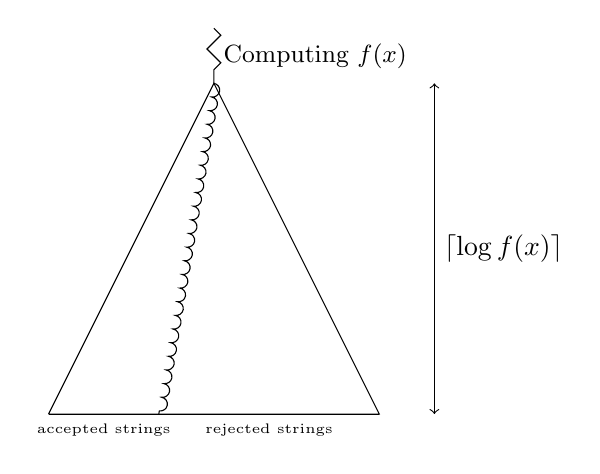
\begin{tikzpicture}[scale=0.7]
\coordinate (T) at (3,7);
\coordinate (A) at (0,0);
\coordinate (B) at (6,0);
\coordinate (C) at (3,6);
\coordinate (M) at (2,0);
\draw [decorate,decoration=zigzag] (T) -> (C) node[midway,right]
{ {\small Computing $f(x)$ }};
\draw (A) -- (M) node[midway,below] { {\tiny accepted strings}} ;
\draw (M) -- (B) node[midway,below] { {\tiny rejected strings}} ;
\draw (A) -- (B) -- (C) -- (A);
\draw [decorate,decoration=bumps] (C) -> (M);
\draw [<->] (7,0) -- (7,6) node[midway,right] {$\lceil \log f(x) \rceil$};
\end{tikzpicture}
\end{figure}

It can be observed that if function computation can be done in polynomial time
then $\P = \NP$. This is because solving decision problem amounts to checking
if the corresponding counting function gives a non zero value or not hence
making decision problem easy if function computation is in \P. 
\begin{lemma}
$\#\P = \FP \implies \P = \NP$
\end{lemma}

An interesting question would be to ask if the converse it true? That is 
\begin{center}
Does $\P = \NP \text{ imply }  \#\P = \FP ?$
\end{center}
We will address this and show a weaker implication (that is, based on slightly stronger LHS) in the next lecture.


\newpage \Lecture{Prasun Kumar}{Jan 12, 2012}{5}{$\FP$ vs $\#\P$ question}
%\theme{ Between $\P$ and $\PSPACE$.}
%\lectureplan{ $\FP$ vs $\#\P$ question, a counter part in the decision world. The class PP. PP vs P is equivalent to FP vs $\#\P$.}

We know $(\#\P = \FP) \implies (\P = \NP)$. In the last lecture we left the question about the converse.
i.e., is it true that, $(\P = \NP) \implies (\#\P = \FP)$?

In this lecture, we will show a weaker version of the above containment.
We will define a new class of languages $\PP$ (probabilistic polynomial time)
in decision world, that contains $\NP$, and will show that if we make a stronger assumption $\PP = \P$ (seemingly stronger than $\NP = \P$) we get the required implication.  We will show in particular that $\PP = \P \iff \#\P = \FP$.

\section{Complexity Class \PP}
For exploring the complexity class, we revisit the definition of $\NP$.
With respect to a "branching" Turing machine(NTM) (which can branch at each computation by using a guess bit), we have two different classes of languages as follows, which differs in their acceptance conditions. We denote for a machine $M$, by $\#acc_M(x)$ as the number of accepting paths. Let the machine run for $p(n)$ time on each path.
\begin{itemize}
\item $\NP$ = $\{$L : $\exists$ branching TM $M_1$, x $\in$ L $\iff \#acc_{M_1}(x) \ge 1 \}$.
\item $\coNP$ = $\{$L : $\exists$ branching TM $M_2$, x $\in$ L $\iff \#acc_{M_2}(x) \ge 2^{p(n)} \}$.
\end{itemize}

In terms of number of accepting paths on input $x$, the above classes
represent the extremes.  On one side, in $\NP$ we talk of atleast one
accepting path, and on the other side, in $\coNP$ we talk of all
accepting paths. To understand the structure of these classes we can
ask the variant of this as : what different class of languages do we
get if we set the accepting condition as the number of accepting paths
being more than a fraction of the total number of paths on input {\em
  x}. A simpler situation is to consider the fraction to be half and the
corresponding class of languages is called \PP (probabilistic
polynomial) which is defined as follows. We will come across other variants in
the later lectures.

\begin{definition}
$\PP$ =$\{$L : $\exists$ NTM $M$, x $\in$ L $\iff \#acc_{M_1}(x) > 2^{p(n)-1} \}$
\end{definition}

We first understand this complexity class with respect to the other ones we have already seen. We start with the following proposition.

\begin{proposition}
\label{prop}
$\NP \subseteq \PP$.
\end{proposition}
\begin{proof}
Let $L \in \NP$  via a nondeterministic turing machine $M$,  $ x \in L \iff M$ has atleast one accepting path on $x$. 
Our aim is to give another turing machine $M'$ for the same language $L$ such that
$x \in L \iff M'$ has more than half of the total number of paths as accepting paths on $x$.\\
Description of $M'$ (on input $x$):
\begin{enumerate}
\item Simulate $M$ on $x$.
\item If $M$ accepts then choose one bit nondeterministically and accept in both branches.
\item If $M$ rejects then choose one bit nondeterministically,accept in one branch and reject in other.
\end{enumerate}

As we remarked in the last lecture, we can assume without loss of generality that the height of computation tree of $M$ on $x$ is exactly $p(n)$ for some polynomial $p$. Since the total number of paths for $M'$ on input $x$ is $2^{p(n)+1}$, it suffices to prove that $x \in L \iff \#acc_M(x) > 2^{p(n)}$.
Let $x \in L$. Since $M$ has at least one accepting path on $x$. Since $M'$, by construction, creates an imbalance (in count) between the number of accepting and rejecting paths precisely when $M$ accepts,  the number of accepting paths in $M'$ will be more than the number of rejecting paths. Thus $\#acc_M(x) > 2^{p(n)}$. \\
If  $x \not\in L$, all paths reject in $M$ on input $x$, and thus  number of accepting and rejecting
paths in $M'$ on input $x$ are exactly equal and each of themsame is equal to $2^{p(n)}$.
\end{proof}

A similar proof will also show that $\coNP$ is contained in
$\PP$. Thus we have the following containment relationship among
different classes of languages
 
\begin{center}
\PSPACE \\ 
$\vert$ \\
\PP \\
$\vert$ \\
\NP \\
$\vert$ \\
\P
\end{center}

Now we will prove the main theorem of the lecture which characterizes the $\FP$ vs $\#\P$ question in the decision world.

\begin{theorem}
 $(\#\P = \FP) \iff (\PP = \P)$
\end{theorem}
\begin{proof}
($\Rightarrow$) Assume $\#\P = \FP$, our aim is to prove $\PP = \P$. The reverse containment follows since we know $\NP \subseteq \PP$ by proposition\ref{prop}. Now we show that $\PP \subseteq \P$ . Let $L \in \PP$
via a machine $M$ running in time $p(n)$ for some polynomial $p$, such that $x \in L \iff \#acc_M(x) > 2^{p(n)-1}$.
Define the function, $f(x) = \#acc_M(x)$. By definition $f \in \#\P$ and hence $f \in \FP$. There is a deterministic polynomial time Turing machine $N$ which on input $x$ outputs the value of $f(x)$. Given an $x$, to test whether it is in $L$ or not, it suffices to test whether whether the MSB of the binary representation of $f(x)$ is 1 or not. This can be done by simply running the machine $N$ on $x$ and testing the MSB of the output. Hence $L \in P$.

($\Leftarrow$) Assume $\PP = \P$, our aim is to prove $\#\P = \FP$. The reverse direction is easy. $\FP \subseteq \#\P$ as we argued in the last lecture. To show the forward direction, let $f\in \#\P$ via $M$ such that $\forall x \in \Sigma^*$, $f(x)=\# accept_M(x)$. Note that the naive approach to compute $f(x)$ is to compute the number of accepting paths in computation tree of height $p(n)$ will take exponential time. But it suffices to find the minimum $0 \le k \le 2^{p(n)}$ such that :
\begin{equation}
\label{eqn}
k+\#acc_M(x) > 2^{p(n)}
\end{equation}
Indeed, the minimum is achieved when $k = k_{min} = 2^{p(n)} - \#acc_M(x) + 1$. Thus $\#acc_M(x) = 2^{p(n)} - k_{min} +1$. This is an indirect way of finding out $\#acc_M(x)$ and we are moving towards using our assumption that $\PP = \P$.

We have  search problem in hand; to search for the minimum $k$($k_{min}$) satisfying equation (\ref{eqn}). We do this by binary search over the range $0 \le k \le 2^{p(n)}$. We solve the decision problem first. {\sf Given $x$ and $k$, check if $k+\#acc_M(x) > 2^{p(n)}$}.

For this, we construct an another Turing machine $N$ such that the number of accepting paths is exactly $k+\#acc_M(x)$ and the total number of paths is $2^{p(n)+1}$. Assume such a construction exists. Define a language $A \subset \Sigma^*$ such that $x \in A \iff k+\#acc_M(x) > 2^{p(n)}$. Thus $x \in A \iff \#acc_N(x) > 2^{p(n)}$. This implies that $A \in PP$ (via the machine $N$ !) and hence $A \in P$ by assumption. Given $x \in \Sigma^*$ we can test if $k+\#acc_M(x) > 2^{p(n)}$ by testing if $x \in A$ or not, which can be done in polynomial time. Now we can do this construction and simulation through a binary search in order to find the minimum value of $k$ that satisfies our inequality.

To complete the proof, we give the construction of $N$ (for a given $k$). 
We first construct a machine $M_k$ that runs in time $p(n)$ and has exactly $k$ accepting paths. 
We slightly modify the idea in the previous lecture to do this. Let $\ell = \lceil \log k \rceil$.
The machine $M_k$ guesses a $y \in \{0,1\}^{p(n)}$ and {\em accepts} if the first $\ell$ bits of $y$ in binary represents a number less than $k$ and the last $p(n)-\ell$  bits is all-zero (lexicographically first path) and {\em reject} otherwise.

We combine $M_k$ and $N$ (both using exactly $p(n)$ non-deterministic bits), to get the machine $N$. The machine $N$ on input $x$ guesses $1$ bit and on the $0$-branch it simulates $M_k$ on $x$ and on the $1$-branch it simulates $M$ on $x$. Clearly $\#acc_N(x) = \#acc_{M_k}(x) + \#acc_{M}(x) = k+\#acc_{M}(x)$. The length of each path is exactly $p(n)+1$ and hence total number of paths is $2^{p(n)+1}$.
\end{proof}




\newpage \Lecture{Sunil K S.}{Jan 13, 2012}{6}{$\#\P$-Completeness}
%\theme{Between $\P$ and $\PSPACE$.}
%\lectureplan{Structure of Reduction in Counting world}

Thus we motivated to answer the questions. We saw $(\#\P=\FP) \iff (\P=\PP)$ in decision world. 
This motivates understanding structure in the counting world.
We start with the notion of reductions. 

\section{Reduction in Counting World}

Our aim is to come up with a notion of $\#\P$-completeness and show structural classification of counting problems. Informally, we have seen counting problems that are hard to solve. We want our notion of hardness to capture this as closely as possible. We consider some natural options for such a definition and proceed from there.

\begin{description}
\item{\textbf{Attempt 1:}}
	Let A,B be two languages. In decision world $A \leq ^p_m B$ if and only if
	\begin{enumerate}
		\item $x\in A\Longleftrightarrow \sigma\in B$.
		\item $\sigma : \Sigma ^*\rightarrow\Sigma^*$ is polynomial time computable.
	\end{enumerate}
	Translating the above statements into counting scenario.
	\begin{enumerate}
		\item $\sigma$ is polynomial time computable.
		\item $f(x)=g(\sigma(x))$.
	\end{enumerate}
	Two lectures back we showed $\SAT$ can be decided if $\#CYCLE$ can be computed. But following the above attempted notion of a reduction, we get the following.
\begin{equation}
\label{eqn:parsi}
	\#\SAT(\phi)=\#CYCLE(\sigma(\phi))
\end{equation}
	
	But if such a reduction exists, then we can solve $SAT$ by checking if $\#SAT(\phi)=\#CYCLE(\sigma(\phi))$, which in turn can be done in polynomial time. Thus, if we impose this strictness then in $\#\P$ only counting versions of $\NP$-complete problems will be hard. Notice that the issue here is that the reduction is set to preserve the number of certificates !. %The reductions which has this property are called {\em parsimonious} reductions.
	
	Let us make some preliminary observations. What if we allow factors in equation\ref{eqn:parsi}? Could this save us? No, still if such a reduction exists, we can decide $\SAT$  by counting the value of $\#CYCLE$. Indeed, there would not have been a problem if there was a "+1" on the right hand side of the above expression, such that the zeroness of $\#\SAT$ does not carry over to the zeroness of $\#CYCLE(\sigma(\phi))$. This shows that may be we should allow non-trivial computations after the query to the function $\#CYCLE$. Since we would also like structural composibility and transitivity of reductions, this naturally leads to the attempt 2, in its generality.
	
\item{\textbf{Attempt 2:}}
We attempt now a generalization of the notion of Turing reductions.
\begin{definition} 
	We say that a function $f \leq g$ if $f\in FP^g$. That is, if there exists a functional oracle Turing machine\footnote{A functional oracle TM is similar to the normal oracle Turing machine, but since the output of the oracle query is not a 1-bit, instead of $q_{yes}/q_{no}$ as the two states to which the machine moves after the oracle answers, the machine has has an oracle output tape for the oracle to write the function value.} 
with queries to $g:\Sigma^*\rightarrow$ $\mathbb{N}$ that given any $x\in \Sigma^*$ can compute $f(x)$. 
	\\A function $g$ is $\#\P$-hard if $\forall f\in \#\P, f\leq_m^p g$. $g$ is complete for $\#\P$ if $g \in \#\P$ and $g$ is $\#\P$-hard.
\end{definition}
\end{description}

\begin{theorem}
 $\#\SAT$ is $\#\P$-complete.
\end{theorem}
	\begin{enumerate}
		\item $\#\SAT \in \#\P$: $\exists$ a non-deterministic turing machine polynomial time which guesses assignments (bit by bit), verifies the same, accepts if it satisfies the formula, and rejects otherwise. No assignment is guessed by two different non-deterministic computation paths. Hence the number of accepting paths will precisely be equal.
		\item $\forall f \in \#\P, f \leq_m^p \#\SAT$: Let $f\in \#\P$ via a machine $M$ such that $\forall x \in \Sigma^*, f(x)=\#acc_M(x)$.
	\begin{description}
	\item \textbf{Cook-Levin Theorem - Revisited.}
	\begin{center}
	$L\in \NP \Longrightarrow L\leq^p_m \SAT$.
	\end{center}
	Let $L\in \NP$, via machine $M$ such that $x\in L \Longrightarrow M$ has an accepting path.
	We construct $\phi_{(M,x)}$ from computation history such that 	$ M$  has an accepting path implies $ \phi_{(M,x)}$ is satisfiable. For every accepting path, we have a satisfying assignment and for every satisfying assignment there is a corresponding accepting path too. Moreover, this map is There is a one-to one mapping between the set of accepting paths and the set of satisfying assignments. The certificates corresponds to the first set is the choice of non-deterministic bits and for the second set is the satisfying assignments. Such reductions are called \emph{Parsimonious reductions}. An additional point is that this certificate bijection is polynomial time computable. That is given an accepting path of the machine $M$ the reduction also gives you a way to transform it into a satisfying assignment of the formula and vice versa. Reductions satisfying the latter property are called {\em Levin reductions}. Note that, in order to prove $\NP$-completeness, the reduction neither need to be parsimonious nor it should be Levin reduction. It is an additional structural property that the reductions seems to satisfy. Interestingly, the $\NP$-complete reductions that we have seen in the last course (like the SAT to 3SAT, 3SAT to independent set, Independent set to Vertex Cover), has this additional structural property. Thus all of them are $\#\P$-complete by our definition.
\end{description}
\end{enumerate}

We have already talked out one example of a decision problem which is in $\P$, but the counting version seems to be as hard as $\NP$. We will consider another similar problem  and show that the counting version can be shown to be $\#\P$-complete as well. Indeed $\#CYCLE$ is also $\#\P$-complete. We introduce the problem now:

\section{Perfect Matching in a graph}
	\begin{definition}: Perfect Matching: 
	Let $G=(X,Y,E)$ be a bipartite graph. A subset $S \subseteq E$ is said to be a perfect matching iff
		\[ \forall u \in X \cup Y : \exists ! v : (u,v) \in S \]
		In words, each vertex has exactly one edge from $S$ incident on it.
	\end{definition} 
We will show a connection that the perfect matching has, with the following combinatorial parameter of the bipartite adjacency matrix. We state this parameter for an arbitrary matrix first.
	\vspace{5mm}
	\begin{definition}: Permanent of a Matrix  
	For an $n\times n$ matrix A, 
\\	Determinant of A, $Det(A)=\displaystyle\sum_{\sigma\text{ is a permutation}\in S_n} (-1)^{sign(\sigma)}\prod_{i=1}^n A_{i,\sigma(i)}$
\\	Permanent of A, $Per(A)=\displaystyle\sum_{\sigma\in S_n} \prod_{i=1}^n A_{i,\sigma(i)}$
	\end{definition}
	
Notice that the parameter is very similar to the determinant of the matrix $A$ which is written as $Det(A)=\displaystyle\sum_{\sigma\in S_n} (-1)^{sgn(\sigma)} \prod_{i=1}^n A_{i,\sigma(i)}$
where $sgn(\sigma)$ assigns a sign to each term based on the sign of the permutation.
Observing the differences, permanent of the 0-1 matrix can never be negative, where as that of a determinant of a 0-1 matrix can be negative. Determinant can be computed in $\FP$, whereas we will show the permanent cannot be computed efficiently unless $\#\P = \FP$.

For a bipartite graph $G$, let $A$ be the bipartite adjacency matrix in which rows are indexed by $x$ 
and columns are indexed by $y$. Note that here $|x|=|y|$, otherwise graph does not have a perfect matching.
Now we will show the following connection:
	
\begin{lemma} 
Let $G$ be the bipartite graph $G$, and let $A$ be the bipartite adjacency matrix of $G$. Then,
$$Per(A)=\#PM(G)$$
\end{lemma}
\begin{proof}
We show that, for any $\sigma$, $\displaystyle\prod_{i=1}^n A_{i,\sigma(i)}=1$ if and only if $\sigma$ gives a perfect matching in $G$.  By definition, $A_{i,\sigma(i)}=1 \iff (i,\sigma(i))\in E$. Since the entries are Boolean, and the product is 1, it must be the case that if $\displaystyle\prod_{i=1}^n A_{i,\sigma(i)}=1$ then all edges $A_{i,\sigma(i)}$ are present in the graph. Since $\sigma$ is a permutation, it must provide an edge $(i, \sigma(i)$ for each vertex $i \in [n]$. Conversely, let $S$ be a perfect matching. It must provide an edge for every $i \in [n]$, and since the perfect matching does not allow any vertex to be covered for more than once, and covers every vertex, we can define a permutation $\sigma$ such that $\sigma(i) = j$ if $(i,j) \in E$. By our observation, $A_{i,\sigma(i)}=1$ as well. Hence the proof.
\end{proof}

Note that the problem of testing whether there exist a perfect matching or not can be done in polynomial time, by using Floyd-Warshall flow algorithm. Thus testing whether perfect matching is zero or not can be done in polynomial time.
But what about computing the value of the permanent function exactly? Is this in $\#\P$ at least? We design a non-deterministic Turing machine: given the matrix $A$, guess the permutation $\sigma$, and check if $\displaystyle\prod_{i=1}^n A_{i,\sigma(i)}=1$, and if so accept and reject otherwise. The number of accepting paths is precisely the number of permutations which contributes 1 to the $Per(A)$. Hence $Per \in \#\P$. Indeed, one can also see this by observing that counting the number of perfect matchings in a bipartite graph is in $\#\P$ (guess a subset of edges and check if it is a perfect matching). We will show soon that $Per$ is $\#\P$-complete too.

Before we end this lecture, let us talk about matrices with non-Boolean entries. Let us say $A \in \Z^{n \times n}$.
Is the permanent function in $\#\P$? An obvious difficulty seems to be that the value of the function can be negative, since the entries could be negative, and it does not make sense to ask for a machine to have negative number of accepting paths. Thus our condition is too stringent, we should relax and ask for can we compute permanent with an oracle access to $\#\P$. We will address these in detail in the next class where we introduce a similar combinatorial interpretation of permanent and use that to argue the $\FP^{\#\P}$ upper bound for computing permanent of integer matrices.


\newpage \Lecture{Dinesh K.}{Jan 16, 2012}{7}{A Combinatorial Interpretation of Permanent}
%\theme{Between $\P$ and $\PSPACE$.}
%\lectureplan{Combinatorial interpretation of permanents over integer
%matrices, using cycle cover}

\newcommand{\countervalue}[1]{\arabic{#1} \addtocounter{#1}{1}}
\newcommand{\perm}{{\sf perm}}
We consider the problem of computing the permanent of a square matrix $A_{n
\times n}$ defined as
\[ \perm(A) = \sum_{\substack{\sigma \in S_n}} \prod_{\substack{i = n}}^n
A_{i, \sigma(i)} \]
where $S_n$ denotes the set of all permutations of $\left \{1, 2, \ldots, n
\right \}$. Note that this formula is very similar to that of the determinant
computation which can be expressed as,
\[ |A| = \sum_{\substack{\sigma \in S_n}} sign(\sigma) \prod_{\substack{i = n}}^n
A_{i, \sigma(i)} \]
where $sign$ of a permutation is $-1/+1$ depending on if the number of inversions
in the permutations is odd or even. 
Though the definitions are similar "syntactically", the computation problems are very different
in the level of hardness. In this lecture, we try to understand more on
permanents and will come up with equivalent combinatorial characterisations.

\section{Characterisation of Permanents of Binary Square Matrices}
Our aim is to how characterise the problem of computing permanent as a
combinatorial problem thereby gives us a handle for attacking the problem. 

Consider a bipartite graph $G(X, Y, E)$ where $|X|=|Y| = n$. Consider the
adjacency matrix $A=(A_{i,j})_{n \times n}$ where,
\[ A_{i,j} = \left \{
	\begin{array}{rl}
	 1 & \text{if } (x_i,y_j) \in E, x_i \in X, y_j \in Y \\
	 0 & \text{otherwise}
	\end{array} \right . \]
We give the following characterisation for permanent of $A$.
\begin{lemma}
$\perm(A) = \left | \text{\# of perfect matchings in } G \right |$
\end{lemma}
\begin{proof}
We show that every permutation $\sigma \in S_n$ corresponds to a unique
perfect matching $\calM$.

($\Rightarrow$) Note that every permutation $\sigma$ of $S_n$ with the property
$\prod_{\substack{i=1}}^n A_{i, \sigma(i)} = 1$ means that there is an edge
connecting vertices $x_i$ and $y_{\sigma(i)}$. Since $\sigma$ is a permutation,
the map is bijective and $y_{\sigma(i)}$ exists for every $x_i$ and is
unique. Hence by definition $\{(x_i, y_{\sigma(i)})| i \in \{1, 2, \ldots,
n\}\}$ forms a perfect matching. 

($\Leftarrow$) Similarly, given a perfect matching $\calM$,
one can define a permutation from $X$ to $Y$ as $\sigma(i)=j$ if $(x_i, y_j)
\in \calM$. It can be seen that the map is bijective and $\prod_{i=1}^n A_{i,
\sigma(i)}$ will be $1$. 

Hence for every $\sigma \in S_n$,
\begin{equation} 
\label{eq:arg}
\prod_{\substack{i=1}}^n A_{i,\sigma(i)} = 1 \iff \left \{ (x_i,
y_{\sigma(i)}) | i \in \{1, 2, \ldots, n \} \text{ is a matching} \right \} 
\end{equation}
Now taking sum over all permutations (on both sides) would give the lemma.
\end{proof}

Hence for a $\{0,1\}$ square matrix, checking if \perm~ is larger than $0$ can
be solved by showing a perfect matching in the corresponding graph.
Standard flow algorithms like the \emph{Fork-Fulkerson algorithm} can be used to find the 
matching in polynomial time.

This characterisation also gives us a \#\P~machine for \perm, thereby showing 
that \perm~is in \#\P.
\begin{lemma}
For $A \in \{0,1\}^{n \times n}$, $\perm(A) \in \#\P$
\end{lemma}
\begin{proof}
Following machine $M$ computes \perm(A).\\
$M$ = ``On input $A_{n\times n}$ 
\begin{enumerate}
\item Construct a bipartite graph $G(X, Y, E)$ with  
$X=\{x_1,x_2,\ldots,x_n\}, \\ Y=\{y_1,y_2,\ldots,y_n\}, (x_i,y_j) \in 
E \iff A_{i,j}=1$
\item Non deterministically guess a subset of edges.
\item Check if they form a perfect matching and accept iff the edges form a
perfect matching."
\end{enumerate}

Note that $M$ runs in polynomial time and by the equivalence~(\ref{eq:arg}),
each perfect matching contributes a count of one to the permanent. Hence the
number of accepting paths of $M$ will exactly be equal to the \perm(A).
\end{proof}

\section{Characterisation of Permanents of Integer matrices}

Now we get to matrices with integer entries. Since the entries could also be negative, the permanent of the matrix 
can be negative. Hence this function cannot be in $\#\P$, but we will show that it is in $\FP^{\#\P}$. 
To do this, we start with the combinatorial characterisation of the permanent, for which we need the notion of cycle covers.

%\subsection{Cycle covers}
\begin{definition}(Cycle Cover) 
Consider a directed weighted graph $G(V,E,w)$ with $w : E
\to \N$. A \emph{cycle cover} of $G$ is a subset of edges that forms a set of vertex disjoint directed
cycles in $G$ such that each vertex is a part of at least one cycle in the cycle cover.

\emph{Weight of a cycle cover} $\calC$ is defined as the product of weights of
edges in $\calC$.
\[ wt(\calC) = \prod_{\substack{e \in \calC}} w(e) \]
\end{definition}

Consider the following examples. Note the effect of adding self loops.
\begin{figure}[htp!]
\centering
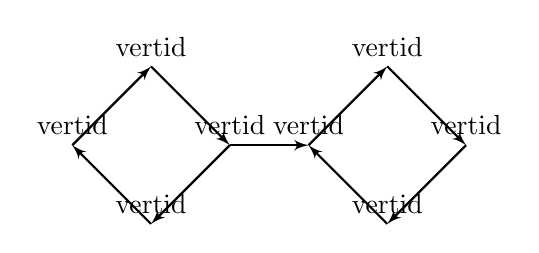
\begin{tikzpicture}
\tikzset{
    myarrow/.style={->, >=latex', thick},
}
\newcounter{vertid}
\setcounter{vertid}{1}
\foreach \x in {0,3}
{
	\draw [myarrow] (\x+1,0) node[above]{\countervalue{vertid}}--(\x+0,1);
	\draw [myarrow] (\x+0,1) node[above]{\countervalue{vertid}}--(\x+1,2);
	\draw [myarrow] (\x+1,2) node[above]{\countervalue{vertid}}--(\x+2,1);
	\draw [myarrow] (\x+2,1) node[above]{\countervalue{vertid}}--(\x+1,0);
};
\draw[myarrow] (2,1) -> (3,1);
\end{tikzpicture}
\quad
\begin{tikzpicture}
\tikzset{
    myarrow/.style={->, >=latex', thick},
}
%\newcounter{vertid}
\setcounter{vertid}{1}
	\draw [myarrow] (1,0) node[above]{\countervalue{vertid}}
	--(0,1.38);
	\draw [myarrow] (0,1.38) node[above]{\countervalue{vertid}}
	--(1,2.76);
	\draw [myarrow] (1,2.76) node[above]{\countervalue{vertid}}
	--(2.62,2.2);
	\draw [myarrow] (2.6,2.2) node[above]{\countervalue{vertid}}
	--(2.6,0.5);
	\draw [myarrow] (2.6,0.5) node[above]{\countervalue{vertid}}
	--(1,0);

\foreach \x in {6.24}
{
	\draw [myarrow] (\x-0,1.38) node[above]{\countervalue{vertid}}
	--(\x-1,0);
	\draw [myarrow] (\x-1,2.76) node[above]{\countervalue{vertid}}
	--(\x-0,1.38);
	\draw [myarrow] (\x-2.62,2.2) node[above]{\countervalue{vertid}}
	--(\x-1,2.76);
	\draw [myarrow] (\x-2.6,0.5) node[above]{\countervalue{vertid}}
	--(\x-2.6,2.2);
	\draw [myarrow] (\x-1,0) node[above]{\countervalue{vertid}}
	--(\x-2.6,0.5);

	\draw [myarrow] (2.6,0.5) -- (\x-2.6,0.5);
	\draw [myarrow] (\x-2.6,2.2) -- (2.6,2.2);

};
\end{tikzpicture}

\centering
\begin{tikzpicture}
\tikzset{
    myarrow/.style={->, >=latex', thick},
}
%\newcounter{vertid}
\setcounter{vertid}{1}
	\draw [myarrow] (1,0) node[above] (A) {\countervalue{vertid}}
	--(0,1.38);
	\draw [myarrow] (0,1.38) node[above] (B) {\countervalue{vertid}}
	--(1,2.76);
	\draw [myarrow] (1,2.76) node[above] (C){\countervalue{vertid}}
	--(2.62,2.2);
	\draw [myarrow] (2.6,2.2) node[above]{\countervalue{vertid}}
	--(2.6,0.5);
	\draw [myarrow] (2.6,0.5) node[above]{\countervalue{vertid}}
	--(1,0);

	\path [myarrow] (A) edge [loop below] (A);
	\path [myarrow] (B) edge [loop left] (B);
	\path [myarrow] (C) edge [loop above] (C);

\foreach \x in {6.24}
{
	\draw [myarrow] (\x-0,1.38) node[above] (E) {\countervalue{vertid}}
	--(\x-1,0);
	\draw [myarrow] (\x-1,2.76) node[above](F){\countervalue{vertid}}
	--(\x-0,1.38);
	\draw [myarrow] (\x-2.62,2.2) node[above]{\countervalue{vertid}}
	--(\x-1,2.76);
	\draw [myarrow] (\x-2.6,0.5) node[above] {\countervalue{vertid}}
	--(\x-2.6,2.2);
	\draw [myarrow] (\x-1,0) node[above](D) {\countervalue{vertid}}
	--(\x-2.6,0.5);

	\draw [myarrow] (2.6,0.5) -- (\x-2.6,0.5);
	\draw [myarrow] (\x-2.6,2.2) -- (2.6,2.2);

	\path [myarrow] (D) edge [loop below] (D);
	\path [myarrow] (E) edge [loop right] (E);
	\path [myarrow] (F) edge [loop above] (F);
}
\end{tikzpicture}
\caption{{\small In the first example, we can see that the only cycle cover is 
\texttt{(1,2,3,4),(5,6,7,8)}. For the second one also there is only one
cycle cover, namely \texttt{(1,2,3,4,5),(10,9,8,7,6)}.
The third is a modified version of the second example. Now there are
\emph{two} cycle covers namely, \texttt{\{(1,2,3,4,5),(10,9,8,7,6)\},
\{(1),(2),(3),(6),(7),(10),(4,5,9,8)\}}}.
}
\end{figure}

We are now set to give a characterisation of permanent over matrices in 
$\Z^{n \times n}$, which we will be crucially using in the next lecture.

\begin{lemma}
Let $A \in \Z^{n \times n}$. Let $G$ be the directed weighted graph obtained
by interpreting $A$ as the weighted adjacency matrix of $G$, i,e. 
\[|V(G)| = n,\] \[ \forall 1 \le i,j \le n, wt(i, j) = w \iff A_{i,j} = w \]
then
\[ \perm(A) = \sum_{\substack{\calC \in Cyclecover(G)}} wt(\calC) \]
\end{lemma}
\begin{proof}
We show that corresponding to every permutation $\sigma \in S_n$, there is a
unique cycle cover $\calC$. That is,
\[ \prod_{\substack{i=1}}^n A_{i,\sigma(i)} = k \iff \exists~\calC \text{ such
that } wt(\calC) = k \]

($\Leftarrow$) Suppose there is a cycle cover $\calC$ such 
that $wt(\calC) = k$. Without loss of generality assume $k \not = 0$. 
(If $k=0$, then one of the edges is not  present and hence no cycle cover is 
possible using the edges in $\calC$).  
Now we can define a permutation to be $\sigma(i) = j~\forall (i,j)\in \calC$.
Since $\calC$ covers all vertices, $\sigma$ is defined for all $\{1,2,\ldots,
n\}$ and since $\calC$ is composed of cycles, every $(i,j)$ will be unique.
Hence the map $\sigma$ will be bijective and is a valid permutation in $S_n$.
Also $\prod_{i=1}^n A_{i,\sigma(i)} = \prod_{(i,j) \in \calC} wt(i,j) =
wt(\calC) = k$.

($\Rightarrow$) Similarly, given a permutation $\sigma$ such that $\prod_{i=1}^n
A_{i,\sigma(i)} = k$, we construct a cycle cover as follows.

If $k=0$, then there is no cycle cover possible with the given permutation
since a zero weight edge is appearing. Hence let $k \not = 0$. Fix an $i\in
\{1,2,\ldots,n\}$. Consider the sequence $(i, \sigma(i), \sigma^2(i), \ldots,
\sigma^n(i))$ where $\sigma^i$ for $i \ge 0$ is obtained by applying $\sigma$
function $i$ times. It can be seen by pigeon hole principle that atleast one
values in the sequence must repeat (since, $\sigma$ is defined on $n$ 
terms and there are $n+1$ terms in the sequence). Without loss of generality, 
let $\sigma^l(i)$ and $\sigma^m(i)$ repeat with $ 0 \le l < m \le n$. 
Since all the weights  are non-zero, the vertices 
$\sigma^l(i), \sigma^{l+1}(i), \ldots, \sigma^m(i) = \sigma^l(i)$ have 
edges between them and clearly forms a cycle. We can find
all the cycles by repeating this process for various values of $i$. 
Note that since $\sigma$ is a permutation, the cycles obtained will be disjoint 
and will cover the entire graph.

Now taking sum over all permutations on both sides proves the claim.
\end{proof}

Using this result the following observation (which is left as an exercise) can
also be made.
\begin{observation}
For $A \in \Z^{n\times n}$ computing permanent of $A$ is in $\FP^{\#\P}$.
\end{observation}

\newpage 
\newcommand{\sP}{\#\P} %% The class #P as it is not defined in complexity.sty
\Lecture{Akshay Degwekar, Devanathan.T}{Jan 17, 2012}{8}{Permanent Computation is \sP-Complete}

\newcommand{\per}{{\sf Per}} % Permanent is defined as an operator.
\newcommand{\wt}{{\sf Weight}} % Weight is defined as an operator.
\newcommand{\integer}{\mathbb{Z}}

In this lecture, we define the permanent of a matrix and study the complexity of computing the permanent for various classes of matrices. Finally we prove a theorem by Valiant that $\per(A)$ is \sP-Complete.

\section{Definitions}
\begin{definition}
\textbf{Permanent } Given a matrix $A_{n \times n}$, Let $S_n$ be the set of
all permutations of $\{1,2,\ldots,n\} = [n]$. Then
\begin{equation}
\per(A) = \sum_{\sigma \in S_n } \prod_{i=1}^n A_{i,\sigma(i)} 
\end{equation}
\end{definition}

Earlier, we have seen a characterization of the permanent as the number of perfect matchings in a graph G. To prove the result, we characterize the permanent using \textbf{Cycle Covers}.

\begin{definition}
\textbf{Cycle Cover } A Cycle Cover $C$ of a directed graph G is a set of pairwise disjoint simple cycles such that each vertex lies in exactly one cycle in $C$.

Note that we allow self-loops as simple cycles.

\xymatrix{
		  & 3 \ar[dr]&	            &   	&	7\ar[dr] \\
2 \ar[ur]& 		 &4\ar[dl]\ar[r]&6\ar[ur]  && 8\ar[dl] \\
&1 \ar[ul]&&&5\ar[ul]&\\}
Has a cycle cover $\big{\{}\{1,2,3,4\},\{5,6,7,8\}\big{\}}$.

\begin{definition}
\textbf{Weight of a Cycle Cover} Given a Graph $G(V,E)$, let $C={C_1, C_2, \dots C_l}$ be any cycle cover
\begin{equation}
\textbf{Weight of Cycle - } \wt(C_i) = \prod_{e\in E}w(e)
\end{equation}
\begin{equation}
\textbf{Weight of Cycle Cover - } \wt(C_i) = \prod_{c\in C}\wt(c)
\end{equation}
\end{definition}


%%That is, In a graph $G(V,E)$, $C = {C_1, C_2, \dots C_l}$ is a cycle cover iff $\forall i,j \quad C_i\cap C_j = \phi$ and $v\in V, \, \exists ! j $ such that $•$ $C_j$ is a 

\end{definition}

\begin{lemma}
Let $G(V,E)$ be a graph with adjacency matrix $A$. 
$A \in \mathbb{Z}^{n\times n}$. Then 
\begin{equation}
	\per(A) = \sum_{\substack{C \text{ is a} \\ \text{Cycle Cover}}} \wt(C)
\end{equation}
\end{lemma}
\begin{proof}
Consider a single term from the permanent - $\sum^n_{i=1}A_{i,\sigma(i)}$.

We can view $\sigma$ as a cycle cover as follows. 

First we decompose $\sigma$ into cycles of the form $a, \sigma(a),
\sigma^2(a)\dots \sigma^k(a) = a$. Now each cycle in the permutation can be
viewed as a cycle in the graph G, the edges being 
\[ \big{\{} (1, \sigma(1)),(2, \sigma(2)), \dots (n, \sigma(n)) \big{\}} \]
This is the required cycle cover. 

For the other direction, some of the cycle covers generated from permutation
might not be valid as some edges are absent. In that case, we just see that 
their weight is 0 as $A_{i,j} = 0$ for the missing edge $(i,j)$. And in the 
case that it is a valid cover, $\wt(C) = \prod_{i\in[n]}A_{i,\sigma(i)}$, because both of them are exactly the product of the corresponding edges.

This shows a bijective correspondence between the permutations and the cycle
covers which completes the proof.
\end{proof}

%%%%%%%%%%%%%%%%Some explanation and notes are required here.

\begin{exercise}
Let $\mathbb{Z}_+$ denote the non negative integers.
Using the previous construction involving cycle covers, 
show that for $A\in \mathbb{Z}_{+}^{n\times n}, \per(A)\in \FP^{\sP}$.

% This problem is also a part of the first problem set.
\end{exercise}


\begin{exercise}
Is the reduction from $\SAT$ to $3\SAT$ parsimonious? If yes, show that
$\#3\SAT$ is $\sP$-complete. 
\end{exercise}

\section{Proof of harndess of Permanent computation}
%Now, we move towards the final part of the lecture - the result by Valiant, that $Per$ is $\sP-Hard$. The proof given here is due to Del.... %add the citations here for both the papers.
In this section, we show that computing permanant of a $0-1$ matrix is $\sP$
complete. The result is due to Valiant~\cite{valiant79}. The proof presented
here is from Dell. et.al~\cite{dell12}. 

We will show this by using a gadget construction.

\begin{theorem}
$\#3\SAT\in \FP^{\per}$
\end{theorem}
\begin{proof}
Consider a formula $\phi $ in $3\SAT$. $\phi = C_1\wedge C_2 \dots C_m$ where $C_i = l_{i,1}\vee l_{i,2} \vee l_{i,3}$.

We will construct a directed graph $G$ such that $A_G$ is the adjacency matrix of $G$, such that $A_G \in \{-1,0,1\}^{n\times n}$ and also, $\per(A_G)=(-2)^k(\#\phi)$ where $(\#\phi)$ is the number of satisfying assignments of $\phi$ and $k$ is a quantity that we specify later.

\begin{lemma}
Let $\#x$ be the number of times a variable $x$ occurs in $\phi$. 

Then $\phi$ can be converted to $\phi'$ such that $\forall x$, $k = \#x=\# \overline{x}$ and $\#phi = \# phi'$
\end{lemma}

\begin{proof}
 We first observe that if $\# x \not = \# \overline{x}$. Then this imbalance can be removed by adding terms of the form $(x\vee x\vee \overline{x})$ and/or $(x\vee \overline{x}\vee \overline{x})$ because they add or decrease the relative number of $x$ compared to $\overline{x}$.
 
 Now, we assume that $\forall x, \#x = \# \overline{x}$.
 Now to compensate for relative differences between $x, y$ we add terms of the form $(x\vee \overline{x}\vee \overline{y})\wedge (x\vee \overline{x}\vee \overline{y})$ to increase the number of $x$ and the other way to decrease.
 
 And we just note that the number of solutions is invariant because each of the added terms are always true.
 
 This completes the lemma.
 \end{proof}
  
  We will be constructing the graph from three gadgets - Variable Gadget, Clause Gadget and the Equality Gadget.

%%% The gadgets  
\begin{figure}[h!]
\centering
%%%%%%%Variable Gadget
\begin{subfigure}[b]{0.3\textwidth}
\xymatrix{ 
	{\bullet}  \ar @/_/ [dd]_x  \ar @/^/ [dd]^{\overline{x}} \\ \\
	{\bullet} \ar [uu]}
	\caption{Variable Gadget}
\end{subfigure} 
%%%%%%%Clause Gadget
\begin{subfigure}[b]{0.3\textwidth}
\centering
 \xymatrix{ 
	 & {\bullet}  \ar @/^/ [d]   \ar @/_/ [ddl]_{\overline{l_1}} & \\ 
	 & {\bullet}  \ar @/^/ [u]  \ar @/^/ [dl]  \ar @/^/ [dr] & \\
{\bullet}\ar @/_/ [rr]_{\overline{l_3}} \ar @/^/ [ur] & & {\bullet}  \ar @/^/ [lu] \ar @/_/ [uul]_{\overline{l_2}} \\	
	}
	\caption{Clause Gadget}
\end{subfigure}
%%%%%%%Equality Gadget
\begin{subfigure}[b]{0.3\textwidth}
\centering
 \xymatrix{ 
	\ar @/_/[ddr] & & {\bullet} \ar@(ul,ur)^{-1} \ar @/_/[ddr] \ar @/_/ [ddl]& & \ar @/^/[ddl] \\ 
	\\
	\ar @/^/[r] & {\bullet}  \ar@(dl,dr)_{1}\ar @/_/ [uur]  \ar @/_/ [rr] & &  {\bullet}  \ar @/_/[uul]  \ar @/_/[ll] \ar@(dl,dr)_{1} & \ar @/_/[l] }
	
	\caption{Equality Gadget}
\end{subfigure}
\caption{The Gadgets}
\label{fig1Gadgets}
\end{figure}

Now, we consider the construction of the graph.

For each variable pair $(x, \overline{x})$ we have one variable gadget. Each clause has a Clause Gadget and the equality gadget is used to join each variable with all the clauses the variable is in.

The equality gadget is represented as a black box as follows -
\begin{figure}[h!]
\centering
\begin{subfigure}[b]{0.3\textwidth}
\centering
 \xymatrix{ 
	\ar @/_/[ddr] & & {\bullet} \ar@(ul,ur)^{-1} \ar @/_/[ddr] \ar @/_/ [ddl]& & \ar @/^/[ddl] \\ 
	\\
	\ar @/^/[r] & {\bullet}  \ar@(dl,dr)_{1}\ar @/_/ [uur]  \ar @/_/ [rr] & &  {\bullet}  \ar @/_/[uul]  \ar @/_/[ll] \ar@(dl,dr)_{1} & \ar @/_/[l] }
	
	\caption{Equality Gadget}
\end{subfigure}
\begin{subfigure}[b]{0.3\textwidth}
\centering
\xymatrix{ 
	\ar @/_/[drr] & \ar @{-} [rrr] \ar @{-} [dd]& & &\ar @{-} [dd] & \ar @/^/[dll]\\
 & & \ar @/_/[dll]&\ar @/^/[drr] & & \\
 & \ar @{-} [rrr]& & & &\\
}	
	\caption{Equality Gadget Representation}
\end{subfigure}
\caption{Equality Gadget Blackbox representation}
\label{fig:EqBlackbox}
\end{figure}

The way we connect a variable and a clause is shown in the next figure. Here $\overline{x}$ is the literal $l_1$ in the clause. 

\begin{figure}[h!]
\centering

\begin{subfigure}[b]{0.3\textwidth}
\centering
\xymatrix{ 
{a}  \ar @/_/ [dd]_x  \ar @/_/[drr]^{u} & \ar @{-} [rrr] \ar @{-} [dd]& & &\ar @{-} [dd] &  & 
{\bullet} \ar @/^/[dlll]^{u'}  \ar @/^/ [d] &  \\ 
 & & \ar @/_/[dll]^{v} &\ar @/^/[drr]^{v'} & &  &  
{\bullet}  \ar @/^/ [u]  \ar @/^/ [dl]  \ar @/^/ [dr] & \\
{b} \ar [uu] & \ar @{-} [rrr]& & & &
{\bullet} \ar @/_/ [rr]^{\overline{l_3}} \ar @/^/ [ur] & & {\bullet} \ar @/_/ [uul]^{\overline{l_2}}  \ar @/^/ [lu] \\	
}	
\end{subfigure}
\caption{Connection between variables and clauses.}
\label{VarClauseConnection}
\end{figure}

When the same variable appears in multiple clauses, we split the edge representing the variable and attach multiple equality gadgets. The next figure shows the split.

\begin{figure}[ht!]
\begin{subfigure}[b]{0.3\textwidth}
\xymatrix{ 
	{\bullet}  \ar @/_/ [ddd]_{\overline{x}}  \ar @/_/ [dr] & & & &  \\ 
& Equality Gadget \ar @/_/ [d] \ar @/_/ [rr] & & Clause Gadget \ar @/_/ [ll]& &\\
& Equality Gadget  \ar @/_/ [dl] \ar @/_/ [rr] & & Clause Gadget \ar @/_/ [ll]& & \\
	{\bullet} \ar [uuu]}
	\label{fig:subfigure1}
\end{subfigure}
	\caption{One variable occurring in multiple clauses.}
\end{figure}

This essentially completes the construction. We will prove the correctness of the construction in a series of claims.
\begin{claim}
Any cycle cover can either use the edge $x$ or $\overline{x}$ in the variable gadget, but not both.
\end{claim}
\begin{proof}
If a cycle cover used both the edges, then the vertices would be covered twice. 
\end{proof}

\begin{claim}
Each assignment corresponds to atleast one cycle cover. 
\end{claim}
\begin{proof}
For each variable, choose $x$ or $\overline{x}$ based on the assignment. And for each clause choose the cycle $l_1 \rightarrow l_2 \rightarrow l_3$ and choose self-loops everywhere else.
\end{proof}

We will derive a much precise correspondence in the remaining proof.


\begin{claim}
In any cycle cover C, either both $u,v$ are used, or neither $u,v$ are used.
\end{claim}
\begin{proof}
The proof is just a verification, We see in \ref{VarClauseConnection} that if the edge $u$ is used, edge $(b,a)$ will have to be used, and to complete a cycle, we will need $v$ to complete the cycle as the edge $x$ cannot be used. 

The proof holds unmodified for edges $u',v'$ too.
\end{proof}

\begin{claim}
If both $u,v$ and $u',v'$ edges are used in the cycle cover, then the $-1$ valued self-loop has to be chosen in the cycle cover. 
\end{claim}

\begin{claim}
If edges $u,v$ are used while $u',v'$ are not used, the corresponding Cycle Covers contribute weight 0.
\end{claim}
\begin{proof}
We just observe that there are two components one contributing $+1$ and the other as $-1$ in the cycle weight. Cycle covers are marked in double lines.

\begin{figure}[H]
\begin{subfigure}[b]{0.3\textwidth}
\centering
 \xymatrix{ 
	\ar @{=>} @/_/[ddr]^{u}  & & {\bullet} \ar@(ul,ur)^{-1} \ar @{=>}@/_/[ddr] \ar   @/_/ [ddl]& & \ar @/^/[ddl]_{u'} \\ 
	\\
	\ar @{<=} @/^/[r]_{v} & {\bullet}  \ar@(dl,dr)_{1}\ar  @/_/ [uur]  \ar @/_/ [rr] & &  {\bullet}  \ar @{=>} @/_/[uul]  \ar @/_/[ll] \ar@(dl,dr)_{1} & \ar @/_/[l]^{v'} }
	\caption{Weight +1}
\end{subfigure}
\begin{subfigure}[b]{0.3\textwidth}
\centering
 \xymatrix{ 
	\ar @{=>}@/_/[ddr]^{u}  & & {\bullet} \ar@{=>}@(ul,ur)^{-1} \ar @/_/[ddr] \ar @/_/ [ddl]& & \ar @/^/[ddl]_{u'} \\ 
	\\
	\ar @{<=}@/^/[r]_{v} & {\bullet}  \ar@(dl,dr)_{1}\ar @/_/ [uur]  \ar @/_/ [rr] & &  {\bullet}  \ar @/_/[uul]  \ar @/_/[ll] \ar@{=>}@(dl,dr)_{1} & \ar @/_/[l]^{v'} }
	\caption{Weight -1}
\end{subfigure}
\caption{Only one of the two sets of edges are present}
\end{figure}
\end{proof}


\begin{claim}
If both $u,v$ and $u',v'$ are not used, then the Cycle Covers have a contribution of 2 from this gadget. 
\end{claim} 
\begin{proof}
The figure \ref{Fig6} contains all the possible cycle covers of the gadget. Their contributions sum upto 2.
\begin{figure}[h]
\begin{subfigure}[b]{0.3\textwidth}
\centering
 \xymatrix{ 
	\ar  @/_/[ddr]^{u}  & & {\bullet} \ar @{=>}@(ul,ur)^{-1} \ar @/_/[ddr] \ar   @/_/ [ddl]& & \ar @/^/[ddl]_{u'} \\ 
	\\
	\ar  @/^/[r]_{v} & {\bullet}  \ar @{=>}@(dl,dr)_{1}\ar  @/_/ [uur]  \ar @/_/ [rr] & &  {\bullet}  \ar @/_/[uul]  \ar @/_/[ll] \ar @{=>}@(dl,dr)_{1} & \ar @/_/[l]^{v'} }
	\caption{Weight -1}
\end{subfigure}
\begin{subfigure}[b]{0.3\textwidth}
\centering
 \xymatrix{ 
	\ar @/_/[ddr]^{u}  & & {\bullet} \ar@{=>}@(ul,ur)^{-1} \ar @/_/[ddr] \ar @/_/ [ddl]& & \ar @/^/[ddl]_{u'} \\ 
	\\
	\ar @/^/[r]_{v} & {\bullet}  \ar@(dl,dr)_{1}\ar @/_/ [uur]  \ar@{=>}@/_/[rr] & &  {\bullet}  \ar @/_/[uul]  \ar@{=>}@/_/[ll] \ar@(dl,dr)_{1} & \ar @/_/[l]^{v'} }
	\caption{Weight -1}
	\end{subfigure}
\begin{subfigure}[b]{0.3\textwidth}
\centering
 \xymatrix{ 
	\ar  @/_/[ddr]^{u}  & & {\bullet} \ar @(ul,ur)^{-1} \ar @{=>}@/_/[ddr] \ar   @/_/ [ddl]& & \ar @/^/[ddl]_{u'} \\ 
	\\
	\ar  @/^/[r]_{v} & {\bullet}  \ar @{=>}@(dl,dr)_{1}\ar  @/_/ [uur]  \ar @/_/ [rr] & &  {\bullet}  \ar @{=>}@/_/[uul]  \ar @/_/[ll] \ar @(dl,dr)_{1} & \ar @/_/[l]^{v'} }
	\caption{Weight 1}
\end{subfigure}	
\begin{subfigure}[b]{0.3\textwidth}
\centering
 \xymatrix{ 
	\ar  @/_/[ddr]^{u}  & & {\bullet} \ar @(ul,ur)^{-1} \ar @/_/[ddr] \ar@{=>}@/_/ [ddl]& & \ar @/^/[ddl]_{u'} \\ 
	\\
	\ar  @/^/[r]_{v} & {\bullet}  \ar@(dl,dr)_{1}\ar  @{=>}@/_/ [uur]  \ar @/_/ [rr] & &  {\bullet}  \ar @/_/[uul]  \ar @/_/[ll] \ar @{=>}@(dl,dr)_{1} & \ar @/_/[l]^{v'} }
	\caption{Weight 1}
\end{subfigure}	
\begin{subfigure}[b]{0.3\textwidth}
\centering
 \xymatrix{ 
	\ar  @/_/[ddr]^{u}  & & {\bullet} \ar @(ul,ur)^{-1} \ar @/_/[ddr] \ar@{=>}@/_/ [ddl]& & \ar @/^/[ddl]_{u'} \\ 
	\\
	\ar  @/^/[r]_{v} & {\bullet}\ar@(dl,dr)_{1}\ar@/_/ [uur]\ar@{=>}@/_/ [rr] & &  {\bullet}  \ar@{=>}@/_/[uul]  \ar @/_/[ll] \ar @(dl,dr)_{1} & \ar @/_/[l]^{v'} }
	\caption{Weight 1}
\end{subfigure}	
\begin{subfigure}[b]{0.3\textwidth}
\centering
 \xymatrix{ 
	\ar@/_/[ddr]^{u}  & & {\bullet} \ar@(ul,ur)^{-1} \ar@{=>}@/_/[ddr] \ar@/_/ [ddl]& & \ar @/^/[ddl]_{u'} \\ 
	\\
	\ar  @/^/[r]_{v} & {\bullet}\ar@(dl,dr)_{1} \ar@{=>}@/_/[uur] \ar@/_/[rr] & &  {\bullet}\ar@/_/[uul]  \ar@{=>}@/_/[ll] \ar@(dl,dr)_{1} & \ar@/_/[l]^{v'} }
	\caption{Weight 1}
\end{subfigure}	
\caption{The weights sum upto 2}
\label{Fig6}
\end{figure}
\end{proof}

\begin{claim}
	Weight of each cycle cover is $(-2)^{kn}$
\end{claim}
\begin{proof}
We want to claim that if a variable $x$ is assigned value $1$, then all the equality gadgets for $x$ will contribute $1$ to the weight because $u,v$ and $u',v'$ will both be a part of the cycle cover for each of the gadgets, if just one pair is in the cycle cover, we have seen that those covers would contribute 0 to the weight. 

Also, the gadgets that correspond to $\overline{x}$ will not have either $u,v$ or $u',v'$ being used - because, $u,v$ cannot be used as $x$ edge will be used, hence $\overline{x}$ cannot be used. Now, if $u',v'$ are used, those cycles will have 0 weight as seen in the observation.

So, the only possibility there is both $u,v$ and $u',v'$ are not used. In that case, the contribution would be $2$ for each gadget. As there are $k$ such gadgets, we will have a contribution of $2^k$ from these. 

So, multiplying them would give us, that each variable pair $x,\overline{x}$ contribute exactly $(-2)^k$ to the weight. Hence the cycle cover would have a weight of exactly $(-2)^{kn}$.

So, We sum them up over all the possible assignments to get the required result. This completes the proof.

\end{proof}

So, we have the result -
\begin{equation}
{\sum_{\text{C is a Cycle Cover}} \wt(C) }= \per_{-1,0,1}(A)
\end{equation}

Hence computing $\#\SAT$ reduces to computing $\per_{-1,0,1}$. This completes the proof. 
\end{proof}

Now we will first show that $\per_{-1,0,1}$ reduces to $\per_{0,1,\dots n}$ and finally show that $\per_{0,1,\dots n}$ reduces to $\per_{0,1}$ and hence completing the theorem.

\begin{theorem}
$\per_{-1,0,1} \in \FP^{\per_{0,1,\dots n}}$.
\end{theorem}
\begin{proof}
 The first thing we observe is that all the -1 terms in the adjacency matrix $A$ represent self-loops because in the construction, $-1$ was the edge weight of only one self-loop.
 
 Consider $\per(A)$ as a polynomial in $x$ where each $-1$ is replaced by $x$ denoted by $p(x)$ 
 
 Now we just observe that, using ${\per_{0,1,\dots n}}$ as an oracle, we can find $p(0), p(1), ... p(n)$. Also, degree of p $\leq n$ because x occurs only in the diagonal entries, hence only n $x $ can be present. 
 
 So, now we just use Lagrange Interpolation to find the polynomial $p$. This can be done in poly time. Once this is done, $\per_{-1,0,1}(A) = p(-1)$, which can be computed easily.
 
 This completes the reduction.
\end{proof}

In the final reduction, we show that $\per_{0,1,\dots n} \in \FP^{\per_{0,1}}$, and that $\per_{0,1}$ is as hard as the other $\per$ computations. 

\begin{theorem}
$\per_{0,1,\dots n} \in \FP^{\per_{0,1}}$
\end{theorem}
\begin{proof}
This proof involves substituting the $-1$ self-loop with a gadget so that we can compute the values of the polynomial $p(x)$ at points $x=0, x=1, \dots x=n$.

The gadget we use is - 
Consider any $a = (a_k, a_{k-1}\dots a_{0})_2$ in base $2$ where $a\in \{0, 1, \dots n\}$. Now we want to replace the self-loop of weight $a$ with the gadget, so that the gadget contributes exactly $k$ weight to the Cycle cover. 

\begin{figure}[ht!]
\xymatrix{
\ar[r]^{1} & \ar@/^/[d]^{a_0} \ar@/_/[r]^{1} \ar@/^/[r]^{1} & \ar@(ul,ur) \ar@/^/[dl]^{a_1} \ar@/_/[r]^{1} \ar@/^/[r]^{1}  & \ar@(ul,ur) \ar@/^/[dll]^{a_2} \ar@[--][r] & \ar@(ul,ur) \ar@/^/[dlll]^{a_{k-1}}   \ar@/_/[r]^{1} \ar@/^/[r]^{1} & \ar@(ul,ur) \ar@/^/[dllll]^{a_{k}} \\ 
& \ar[ul]^{1} & & \\
}
\end{figure}

The gadget has precisely $n$ cycles of weight $1$ each. This gadget can be used to replace the self loop and then query the $\per_{0,1}$ oracle. 

This completes the reduction. Hence proved.
\end{proof}


\newpage 

\newcommand{\paths}[2]{\ensuremath{\#paths_{M}(x)}}
\newcommand{\acc}[2]{\ensuremath{\#acc_{M}(x)}}
\newcommand{\rej}[2]{\ensuremath{\#rej_{M}(x)}}
\newcommand{\err}[2]{\ensuremath{\#err_{M}(x)}}

\newcommand{\ParityP}{\ensuremath{\oplus\P}}

% \newcommand{\iff}{\LeftRightarrow}


\Lecture{Balagopal}{23 Jan, 2012}{09}{Probabilistic TMs and Randomized Algorithms}
%\theme{}
%\lectureplan{}

\section{Review of Branching machines}

A branching machine is a machine that is allowed to make non-deterministic guesses while computation. This is 
a generalization of NTMs where the branching machine accepts iff at least one path accepts. Similarly we can think of 
various definitions of acceptance each of them leading to a (possibly) new complexity class. For example, \PP\ is defined as the class 
which has a branching machine where more than half of the paths accept. \ParityP\ is defined as the class where each language has a 
branching machine in which an odd number of paths accept if $x \in L$. Similarly we can think of every branching machine as computing 
a function $f(x)$ where $f(x)$ is defined as the number of accepting paths of $M$ on $x$.

\textbf{Question. } How is \ParityP\ related to \P\ , \NP\ , \PSPACE\ , and \PP\ ?

We will come back to answer this question, and show that $\NP$ can be
{\em almost} solved in $\P$ if $\ParityP$ can be solved in $\P$. The
{\em almost} here will refer to possibility of error by the algorithm
in the decision. We will now do a systematic formal study of
randomized algorithms (algorithms which may make an error but with low
probability). We introduce these from the branching machine
perspective that we have seen so far.

\section{Characterizing Randomized Algorithms}

We are going to characterize randomized algorithms using branching machines that we 
defined previously.

Consider a branching machine $M$ for the language $L$. If $x \in L$ call all paths of $M$ that 
reject as erroneous. If $x \notin L$ call all paths of $M$ that accept as erroneous. Intuitively, 
we want the erroneous paths to be as small as possible. We use the following notations for counting 
paths with specific properties for a branching machine $M$.

\begin{description}
\item[$\paths{M}{x}$] Total number of paths of $M$ on $x$

\item[$\acc{M}{x}$] Total number of accepting paths of $M$ on $x$

\item[$\rej{M}{x}$] Total number of rejecting paths of $M$ on $x$

\item[$\err{M}{x}$] Total number of erroneous paths of $M$ on $x$
\end{description}

We defined class \PP\ as the set of languages $L$ with branching machines 
satisfying the following property.

\begin{eqnarray*}
x \in L &\implies& P(A \textrm{ accepts } x) > 1/2 \\
x \notin L &\implies& P(A \textrm{ rejects } x) \geq 1/2
\end{eqnarray*}

To connect the notion of a branching program and a randomized algorithm, we have to make sure 
that all paths of the branching machine are of the same length (i.e., the computation tree is a full 
binary tree). This can be done by a construction similar to the one used to do this while defining \#\P.
However, when a path is extended by branching it yields multiple paths. We must ensure that the error probabilities are not 
increased during this process.
Note that this is different from what we did while defining \#\P. 
The goal there was to preserve the count (Number of accepting paths). 
The goal here is to keep the error probability (which depends on the relative number of accepting and rejecting paths) the same.

Now consider a randomized algorithm $A$ that chooses one path of $M$ uniformly at random and 
executes it (This shows that there is a randomized algorithm corresponding to every branching machine). 
Clearly

\begin{equation}
x \in L \iff \err{M}{x} \leq \frac{1}{2} \paths{M}{x}
\end{equation}


We see that the probability of $A$ making an error is at most 1/2. But this can be 
achieved by a trivial randomized algorithm that flips a coin and determines the result according 
to the outcome of the coin flip. So the class \PP\ is not a good candidate for formally capturing 
``good'' randomized algorithms.

What we want is the error probability to be bounded away from $1/2$. If $\err{M}{x} < \frac{1}{4} \paths{M}{x}$, then 
certainly the corresponding randomized algorithm is better than a trivial one.

We will now work towards defining a problem for which there is an efficient (poly time) randomized algorithm but for which 
no poly time deterministic algorithm is known. This gives reason to study randomized algorithms formally.


\section{Polynomial Identity Testing}

This problem has its roots in the simple high school
arithmetic. Suppose we are given a polynomial in a complicated form
where the monomials may repeat with arbitrary coefficients etc. We
want to find out if the coefficient of the monomials cancel out to
zero. This in effect is testing whether the polynomial is the zero
polynomial, and equivalenty it is testing if the polynomials evaluates
to zero on all substitutions of the variable from the underlying field
$\mathbb{F}$.

How are we given the polynomial? This indeed is going to have effect
on the complexity of the problem.  Let us start with the high school
arithmetic again. Suppose we are given it in the monomial form (though
some monomials may repeat) along with their coefficients. To solve the
problem, it suffices to check, for each monomial whether the
coefficient in its various appearences is adding up to zero. Given the
explicit representation at the input, this is very easy to do by
simply going over the input for each monomial. Hence this can be done
in time polynomial in the input.

What if the polynomial is not given that explicity. What is the most
implicit form that we can think of? A black box which evaluates the polynomial.
That is, we have an oracle $p$ when given input $a$ returns $p(a)$, the value of polynomial 
at $a$.

%The aim is to test whether the input polynomial is identically 0 (The zero polynomial). If the polynomial 
%is given as monomials, then we can do this in {\tt poly} time. But what if the input polynomial is given in 
%$blackbox form. 

Assume that we are also given an upper bound on the degree of the
polynomial $deg(p) \leq d$.  Indeed, we do not have access to the
actual polynomial except through the blackbox. We have to use some
property of the degree $d$ polynomials. The most obvious one is the
number of points in which they can evaluate to zero. Based on this thought, 
the following deterministic algorithm solves the problem.

\begin{figure}[ht]
{\tt \obeyspaces \obeylines
1. Choose $d + 1$ different points $a_1 , \ldots , a_{d+1}$.
2. Call the oracle $d+1$ times to evaluate $p(a_1), \ldots , p(a_{d+1})$.
3. If all calls returned 0 accept else reject.
}
\caption{A deterministic algorithm for univariate polynomial identity testing}
\end{figure}

If $p$ were really 0 then all calls will return 0 and we will definitely accept. If $p$ were not 
0, then at most $d$ calls can return 0 since a polynomial with degree at most $d$ has at most $d$ 
roots. Hence if $p \neq 0$, then our algorithm will definitely reject.

Now let us think about the problem when $p$ is a multivariate
polynomial. The previous assertion that a degree $d$ polynomial has at
most $d$ roots no longer holds. To see this, consider the degree 2
polynomial $p(x_1, x_2) = x_1 x_2$. This has an infinite number of
roots $x_1 = 0, x_2 \in \mathbb{F}$, where $\mathbb{F}$ is the
(possibly infinite) field over which $p$ is defined.  We can work
around this problem by considering a finite subset of the field, say
$S = \{ 0, \ldots ,10 \}$. The polynomial $p$ has $19$ zeroes. So if
$x_1, x_2$ is chosen uniformly at random from $S$ there is at most
$19/100$ chance that we will get a false result. As can be seen from
the above example, by making the size of $S$ arbitrarily large, we can
make the error probability arbitrarily small. But then the
disadvantage is that we will need more random bits in order to choose
an element at random from the set $|S|$, and the running time of our
algorithm will also increase.

In the next lecture, we will show that this intuition is correct by
exhibiting a low error polynomial time randomized algorithm for the
multivariate case. The question of finding a deterministic algorithm
for this problem is open. Although it looks like a simple algorithmic
problem from algebra which only mathematicians might be interested in,
there are several computational problems that can be encoded into this
form and hence can be solved efficiently if this algorithmic problem
can be solved efficiently.
 

\newpage \Lecture{Sunil K S}{Jan 24, 2012}{10}{Polynomial Identity Testing}

Towards the end of last lecture, we introduced the following problem :
{\em Given a polynomial $p$, test if it is identically zero}. That is,
do all the terms cancel out and become the zero polynomial. Described
as a language :
$$\textrm{\sc PIT}=\{ p ~|~p \equiv 0\}$$
We also saw some easy cases of the problem:
\begin{enumerate}
\item When it is given as a sum of monomials: Given $p$, run over the
  input to figure out the coefficient of each monomial, and if all of
  them turn out to be zero, then report that $p$ is in {\sc PIT}. This
  algorithm runs in $O(n^2)$ time.
\item When it is given as a Black Box: In uni-variate case, check
  $p(x)$ for $d+1$ different points where $d$ is the degree bound. If
  the polynomial is not equivalent to zero, then at-least one of the
  steps gives a non-zero value. Indeed, if the polynomial is zero,
  then all the $(d+1)$ evaluations will result in a zero value. Thus
  the algorithm is correct and runs in time $O(d)$ where $d$ is the
  degree of the polynomial.
\end{enumerate}

As we observed, this strategy could not be generalized in
multi-variate case. We took an example as $p(x_1,x_2) = x_1x_2$. For
the assignment $x_1=0$, whatever $x_2$ chose, the value will always be
0. However, if $p \equiv 0$, no matter what we choose as the
substitution for $x_1$, and $x_2$, the polynomial will be identically
zero.

The strategy that we will follow is as follows: If the total degree of
the polynomial is $\leq d$, and if $S \subseteq \F$, such that
$|S|\geq 2d$, instead of picking elements arbitrarily, we pick
elements uniformly at random from $S$. Indeed, there may be many
choices for the values which may lead to zero. But how many?
%Here by increasing the size of $S$, we can improve the probability.
% IMPRECISE statement.

\begin{lemma}[Schwartz-Zippel Lemma]
Let $p(x_1, x_2, \cdots , x_n)$ be a non-zero polynomial over a field
$\mathbb{F}$. Let $S\subseteq \mathbb{F}$
$$Pr[p(\bar{a}=0]\leq \frac{d}{|S|}$$
\end{lemma}
%It also shows that the number of solutions for $P(\bar{a})$ if $\leq d|S|^{(n-1)}$.
\begin{proof}
(By induction on $n$) For $n=1$: For a univariate polynomial $p$ of
  degree $d$, there are $\leq d$ roots. Now in the worst case the set
  $S$ that we picked has all $d$ roots. Thus for a random choice of
  substitution for the variable from $S$, the probability that it is a zero of
  the polynomial $p$ is at most $\frac{d}{|S|}$.

For $n>1$, write the polynomial $p$ as a univariate polynomial in $x_1$ with coefficients as polynomials in the variables $p(x_2, \ldots, x_n)$.
$$ \displaystyle \sum_{j=0}^{d}x_1^jp_j(x_2, x_3, \ldots, x_n)$$

For example: $x_1x_2^2+x_1^2x_2x_3+x_3^2=(x_2x_3)x_1^2+(x_2^2)x_1+x_1^0(x_3^2)$.

To analyse the probability that we will choose a zero of the
polynomial (even though the polynomial is not identically zero). For a
choice of the variables as $(a_1, a_2, \cdots, a_n)\in S^n$, we ask
the question : how can $p(a_1, a_2, \cdots, a_n)$ be zero? It could be
because of two reasons:

\begin{enumerate}
\item $\forall j~:~1 \le j \le n , ~~ p_j(a_2, a_3, \ldots , a_n)=0$.
% In this case whatever $(a_2, a_3, \cdots , a_n)=0$, polynomial will be zero.
\item %$(a_2, a_3, \cdots , a_n)=0$.
Some coefficients $p_j(a_2, a_3, \ldots , a_n)=0$ are non-zero, but
the resulting univariate polynomial in $x_1$ evaluates to zero upon
substituting $x_1 = a_1$.
\end{enumerate}

Now we are ready to calculate $Pr [ p(a_1, a_2, \ldots, a_n) = 0 ]$.
%\begin{eqnarray*}
For a random choice of $(a_1, \ldots, a_n)$.
Let $A$ denote the event that the polynomial $p(a_1, \ldots, a_n) = 0$.
Let $B$ denote the event that $\forall j~:~1 \le j \le n ,~~p_j(a_2, a_3, \cdots , a_n)=0$.
Now we simply write : $Pr[A] = Pr[A \land B]+Pr[A\land \bar{B}]$.

We calculate both the terms separately: $Pr[A \land B] = Pr[B].Pr[A|B]
= Pr[B]$ where the last equality is because $B \implies A$.  Let
$\ell$ be the highest power of $x_1$ in $p(x)$. That is $p_\ell \ne
0$. Since the event $B$ insists that for all $j$, $p_j(a_2, a_3,
\ldots , a_n)=0$, we have that $Pr[B] \leq Pr[p_\ell(a_1, a_2, \ldots,
  a_n) \ne 0]$.  By induction hypothesis, since this polynomial has
only $n-1$ variables and has degree at most $\frac{d -
  \ell}{S}$. Thus, $Pr[B] \le \frac{d - \ell}{S}$.

To calculate the other term,
\begin{eqnarray*}
Pr[A \cap \bar{B}] & = & Pr[\bar{B}].Pr[A|\bar{B}] \le Pr[A|\bar{B}] \le \frac{\ell}{|S|}
\end{eqnarray*}
where the last inequality holds because the degree of the non-zero
univariate polynomial after substituting for $a_2, \ldots, a_n$ is at
most $\ell$ and hence the base case applies.
\end{proof}

This suggests the following efficient algorithm for solving PIT. Given $d$ and a
blackbox evaluating the polynomial $p$ of degree at most $d$.

\begin{figure}[ht]
{\tt \obeyspaces \obeylines
1. Choose $S \subseteq \mathbb{F}$ of size $\ge 4d$.
1. Choose $(a_1, a_2, \ldots, a_n) \in_R S^n$.
2. Evaluate $p(a_1, a_2, \ldots a_n)$ by querying the blackbox.
3. If it evaluates to 0 accept else reject.
}
\caption{A randomized algorithm for multivariate polynomial identity testing}
\end{figure}

The algorithm is clearly running in polynomial time. The following
Lemma states the error probability and follows from the
Schwartz-Zippel Lemma that we saw before.
\begin{lemma}
There is a randomized polynomial time algorithm $A$, which, given a black
box access to a polynomial $p$ of degree $d$ ($d$ is also given in unary), answers whether the polynomial is identically zero or not,
with probability at least $\frac{3}{4}$.
%\[ p \not\equiv 0 \implies \textrm{ Pr[$A$ accepts] $\ge \frac{3}{4}$} \]
%\[ p \equiv 0 \implies \textrm{ Pr[$A$ accepts] $= 0$.} \]
\end{lemma}

Notice that in fact the lemma is weak in the sense that it ignores the
fact that when the polynomial is identically zero then the success
probability of the algorithm is actually 1 !.

Now we connect to where we left out from Branching machines, by
observing that this randomized algorithm is indeed a branching machine.
Let $\chi_L(x)$ denote the characterestic function of the
language. That $\chi_L(x) = 1$ if $x \in L$ and $0$ otherwise.  Let us
call a computation path to be {\em erroneous} if the decision ($1$ for
accept and $0$ for reject) reported in that path is not
$\chi_L(x)$.  Let $\#err_M(x)$ denote the number of erroneous paths.
Thus the braching machine has some guarantees about $\#err_M(x)$.
%with some guarantees on the number of erroneous paths.

\begin{corollary}
Let $L$ be the language $PIT$, then there exists a branching machine
$M$, running in $p(n)$ time (hence using at most $p(n)$ branching
bits).
\[ \#err_M(x) \le \frac{1}{4}2^{p(n)} \]
%\begin{eqnarray*}
%x\in L&\Rightarrow&     \#acc_M(x)\geq \frac{3}{4}2^{p(n)}. \mbox{ In case of PIT, it is } =2^{p(n)}.\\
%x\notin L&\Rightarrow&  \#acc_M(x)\leq \frac{1}{4}2^{p(n)}.% \mbox{ } \rightarrow P\neq 0.
%\end{eqnarray*}
\end{corollary}

Is there anything special about $\frac{1}{4}$? As we can go back an
observe, this number can be reduced to say $\frac{1}{5}$ by easily
choosing the size of the set $S$ to be larger than $5d$ where $d$ is
the degree of the polynomial. We get better success probability then,
but what do we lose? We lose on the running time, since we have to
spend more time and random bits now in order to choose the elements
from $S^n$ as $|S|$ has gone up.

But more seriously, this seems to be an adhoc method which applies
only to this problem. In general, if we have a randomized algorithm
that achieves a success probability of $\frac{3}{4}$, can we boost it
to another constant?

Based on the discussion so far, we can make the following definition
of a set of languages. For a fixed $\epsilon$, define the class $\BPP_\epsilon$ as follows.
%\textbf{Bounded error Probabilistic Polynomial time (BPP)}:\\ 
$L \in BPP_{\epsilon}$, for some $0 \epsilon < \frac{1}{2}$, if there is a branching machine $M$
running in time $p(n)$, such that $\#err_M(x) \le \epsilon2^{p(n)}$.

Notice that all these sets of classes are contained in $\PSPACE$. Let $L \in
BPP_{\epsilon}$ via a machien $M$.  By just brute force run over all
the choice bits of the machine $M$ (reusing space across different
paths) we can exactly calculate how many paths are accepting. This
information will be sufficient to decide whether $x \in L$ or not..

All of them contain $\P$ since there is a trivial choice machine which
achieves any success probability (of 1 !).

How do they compare, for different $\epsilon$ and $\epsilon'$? Could
they be incomparable with each other (and hence form an antichain in
the poset of languages)? In the next lecture we will show a lemma
which will imply that for any constants $0 < \epsilon \ne \epsilon' <
\frac{1}{2}$, $\BPP_\epsilon = \BPP_{\epsilon'}$.  This eliminates the
possibility of an antichain in the poset and makes the definition of
the following complexity class.

\begin{definition}[BPP]
A language $L$ is said to be in $\BPP$ if there is an $\epsilon$ such
that $0 < \epsilon \le \frac{1}{2}$, and a branching machine $M$
running in time $p(n)$ such that: $\#err_M(x) \le \epsilon2^{p(n)}$
\end{definition}

We begin the thoughts on proving $\BPP_\epsilon = \BPP_{\epsilon'}$
for $0 < \epsilon \ne \epsilon' < \frac{1}{2}$. Without loss of
generality, assume that $\epsilon < \epsilon'$.  Note that
$\BPP_\epsilon \subseteq \BPP_{\epsilon'}$. To show the other
direction we need to improve the success probability of the
algorithm. Viewing the success of the algorithm as a favourable
probability event, a natural strategy is to repeat the process
independently again, so that the probability of error goes down
multiplicatively. Thus it improves the success probability.


\newpage \Lecture{Princy Lunawat}{Jan 25, 2012}{11}{Amplification Lemma}

In the last lecture, we saw the polynomial identity testing problem
and a randomized algorithm for it. We also discussed how branching machines with
guarantees on the number of erroneous paths characterize randomized
algorithms. We ended the last lecture with a question about how two
sets of languages compare. $\BPP_{\epsilon}$ and $\BPP_{\epsilon'}$.
for different $\epsilon$ and $\epsilon'$? 

\section{Amplification of Success Probability}

We showed that if $\epsilon < \epsilon'$ then $\BPP_{\epsilon} \subseteq \BPP_{\epsilon'}$. A strategy to prove the other direction was the following : Repeat the randomized algorithm (experiment) multiple
times (say $k$), and then take the majority of the outcomes in order to improve our success probability.
One remark is that the repetition is sequential and happens on each
branch. Thus we are essentially producing a new branching machine with
many deeper computation paths. 

Why would this improve the success probability? and if so, how does it depend on $k$?. 
The following lemma answers these.

\begin{lemma}
If $\mathcal{E}$ is an event that $Pr(\mathcal{E}) \geq \frac{1}{2} + \epsilon $, then the probability the $\mathcal{E}$ occurs atleast $\frac {k}{2}$ times on $k$ independent trials is at least 
$1-\frac{1}{2}(1-4\epsilon^2)^\frac{k}{2}$
\end{lemma}
\begin{proof}
Let $q$ denote the probability the $\mathcal{E}$ occurs atleast $\frac {k}{2}$ times on $k$ independent trials.
Let $q_i$ = Pr($\mathcal{E}$ occurs exatly $i$ times in $k$ trials), $0 \leq i \leq k$. Thus,
$q = 1 - \sum_{i=0}^{\lfloor\frac{k}{2}\rfloor}$ $q_i$. We will analyse the complementary event:
Pr($\mathcal{E}$ occurs atmost $\frac{k}{2}$ times) = $\sum_{i=0}^{\lfloor\frac{k}{2}\rfloor}$ $q_i$. \\ 
We show an upper bound on each $q_i$ and thus show an lower bound on $q$.
\begin{eqnarray*}
q_i & = & {k \choose i} (\frac{1}{2} + \epsilon)^{i} (\frac{1}{2} - \epsilon)^ {k-i} \\
& \leq & {k\choose i} \left(\frac{1}{2} + \epsilon\right)^{i} \left(\frac{1}{2} - \epsilon\right)^ {k-i} \left(\frac{\frac{1}{2} + \epsilon}{\frac{1}{2} - \epsilon}\right)^{\frac{k}{2} - i}  (because \epsilon \le \frac{1}{2} ) \\
& = & {k\choose i}\left(\frac{1}{2} + \epsilon\right)^{\frac{k}{2}}\left(\frac{1}{2} - \epsilon\right)^{\frac{k}{2}} \\
&= & {k\choose i} \left(\frac{1}{4} - \epsilon^2\right)^{\frac{k}{2}}
\end{eqnarray*}
Now we analyse the sum:
\begin{eqnarray*}
\sum_{i=0}^{\lfloor\frac{k}{2}\rfloor}q_i & \leq & \sum_{i=0}^{\lfloor\frac{k}{2}\rfloor}{k\choose i} \left(\frac{1}{4} - \epsilon^2\right)^{\frac{k}{2}} \\
q = 1 - \sum_{i=0}^{\lfloor\frac{k}{2}\rfloor}q_i & \geq & \sum_{i=0}^{\lfloor\frac{k}{2}\rfloor}{k\choose i} \left(\frac{1}{4} - \epsilon^2\right)^{\frac{k}{2}} \\
& = & 1 - \left(\frac{1}{4} - \epsilon^2\right)^{\frac{k}{2}} 2^{k-1} \\
& = & 1 - \frac{1}{2} \left(1 - 4\epsilon^2\right)^{\frac{k}{2}} \\
\textrm {Thus, } q & \ge & 1 - \frac{1}{2} \left(1 - 4\epsilon^2\right)^{\frac{k}{2}}
\end{eqnarray*}
\end{proof}

In the last lecture, we defined the class $\BPP_\epsilon$ (Bounded Error Probabilistic Polynimial Time) and now we can use the above amplification lemma to prove that
\[\BPP_{\epsilon} = \BPP_{\epsilon^{'}} \hspace{3mm}\forall  0 \leq \epsilon , \epsilon' < \frac{1}{2} \]

We want to calculate
In general, the above lemma can be used to prove that , at the cost of running time, the the error probability of a language $L$ , 
$L \in \BPP$ can be reduced to $\frac{1}{2^{q(n)}}$ where $q(n)$ is a polynomial in $n$.
 
\begin{lemma}
$L \in \BPP$ if an only if for any polynomial $q(n)$ there is a machine $M$ that runs for time $p(n)$ (which depends on $q(n)$) such that \\
\[ \textrm{ Pr($M$ errs on input $x$)) } \le 2^{-q(n)} \] 
In terms of number of paths,
\[ \#err_M(x) \le  2^{p(n)-q(n)} \]
\end{lemma}
\begin{proof}
Given a language $L \in \BPP_\epsilon$ with PTM $M$, we design a PTM $N$ such that $L(N) \in \BPP$ and $L(n) = L$ as follows:
\begin{itemize}
 \item Run the machine $M$ on input $x$ $k$ times independently where choice of $k$ is such that
\\
\begin{equation}\label{eq:eq2}
 \frac{1}{2} \left(1 - 4\epsilon^2\right)^{\frac{k}{2}} \leq 2^{-q(n)}
\end{equation}

\end{itemize}
The above equation $\eqref{eq:eq2}$ yields a value of $k$ polynomial in $n$ and hence $N$ runs a polynomial number of times.
The amplification lemma ensures that the error probability reduces to the LHS of the equation $\eqref{eq:eq2}$.
\end{proof}

\section*{The Structure of \BPP}
We explore some interesting structural properties about the class $\BPP$.

\begin{proposition}
$\BPP$ is closed under complementation.
\end{proposition}
\begin{proof}
Let $L \in BPP$ via PTM $M$ with error probability $\epsilon < \frac{1}{2}$ . We show that $\bar L$ is in $\BPP$.
We design a new machine $\bar M$ by switching the accept and reject states of $M$.
\begin{eqnarray*}
x \in L & \implies & \#acc_M(x) \geq (1 - \epsilon )\#path_M(x) \\
& \implies & \#rej_M(x) \leq \epsilon \#path_M(x). \\
& \implies & \#acc_{\bar M} \leq \epsilon \#path_{\bar M}(x). \\
& \implies & x \notin L(\bar M). \\
x \notin L & \implies & \#acc_M(x) \leq \epsilon.\#path_M(x). \\
& \implies & \#rej_M(x) \geq (1-\epsilon)\#path_M(x). \\
& \implies & \#acc_{\bar M} \geq (1-\epsilon) \#path_{\bar M}(x).\\
& \implies & x \in L(\bar M).
\end{eqnarray*}

Hence, we have,
\[x\in L \iff x\notin L(\bar M) \]
Therefore, $L(\bar M) = \bar L$ and $L \in BPP$ via machine $\bar M$. Hence,
$BPP$ is closed under complementation.
\end{proof}

%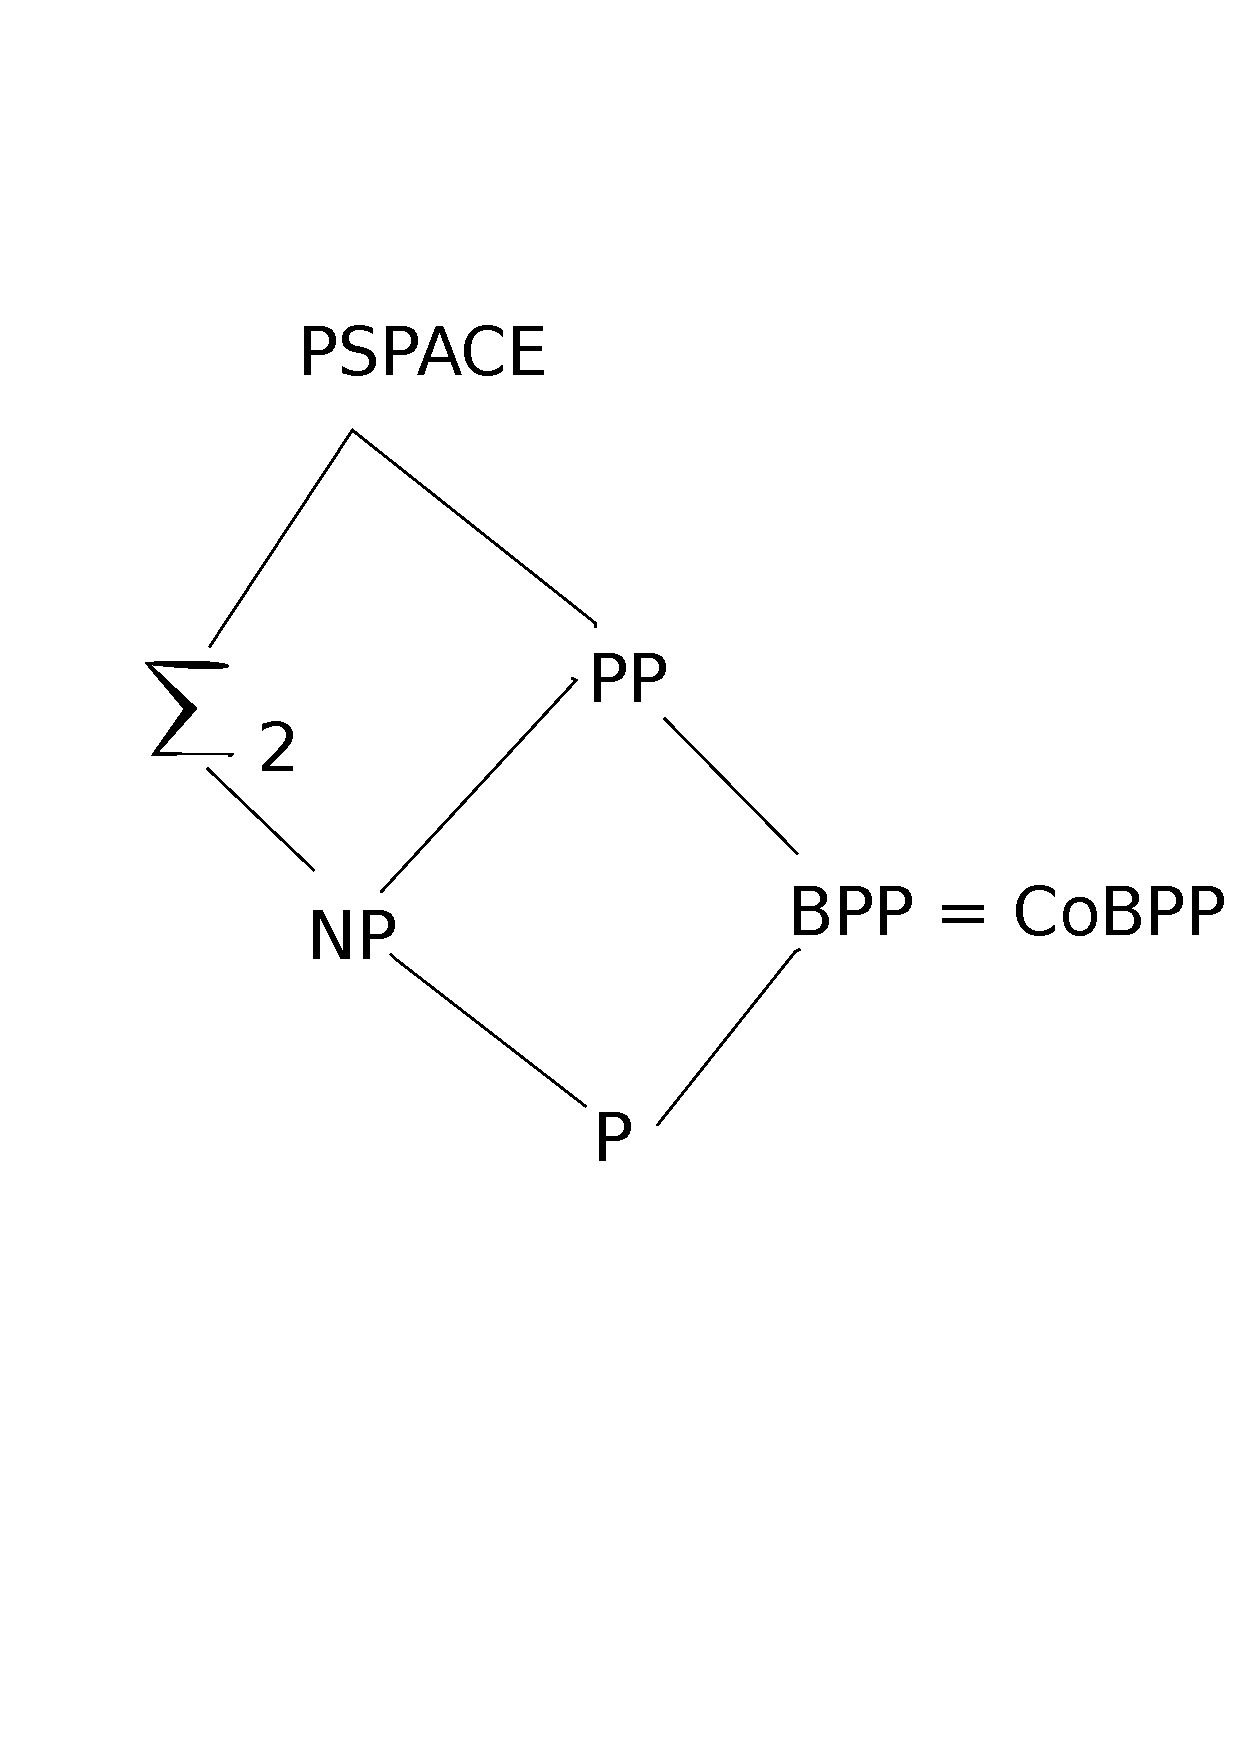
\includegraphics[scale=0.5,trim = 10mm 80mm 50mm 5mm]{hie1}
%\pagebreak

\section*{One-sided Error Randomized Algorithms}

Consider the language , PIT that is, Polynomial Identity Testing,
\[PIT =\{ p |  p\equiv 0 \}\] where $p$ is a polynomial.
From, the last lecture, we make the following observation about PIT,
if $p \in PIT$, PTM makes no error,
if $p \notin PIT$, PTM makes some error (less than half the number of paths).

We now explore how complexity theory can be extended to these kind of algorithms too.
\begin{definition}({\bf \RP})
A language $L$ is said to be in $\RP$ if there is an $\epsilon$ such
that $0 < \epsilon < \frac{1}{2}$, and a randomized algorithm $A$ such that :
\begin{eqnarray*}
x \in A & \implies & Pr [\textrm{ $A$ accepts }] \ge \frac{1}{2}+\epsilon \\
x \notin A & \implies & Pr [\textrm{ $A$ accepts }] = 0
\end{eqnarray*}
\end{definition}

Hence we have the following proposition:
\begin{equation}
PIT \in \co\RP
\end{equation}

\begin{proposition}
$\RP \subseteq \NP$
\end{proposition}
\begin{proof}
Consider language $L \in \RP$ via machine $M$ such that 
$x \in L \implies M $ accepts $x$ with some error $\epsilon < \frac{1}{2}$
$\implies M $ accepts $x$ on atleast 1 path. \\
$x \notin L \implies M$ accepts $x$ with probability 0 $\implies M$ rejects on all paths.
Thus $L \in \NP$. Moreover, even with the acceptance condition of a non-deterministic machine, the branching machine corresponding to the $\RP$ algorithm accepts the language $L$ itself.
\end{proof}
\vspace{-40mm}
\begin{center}
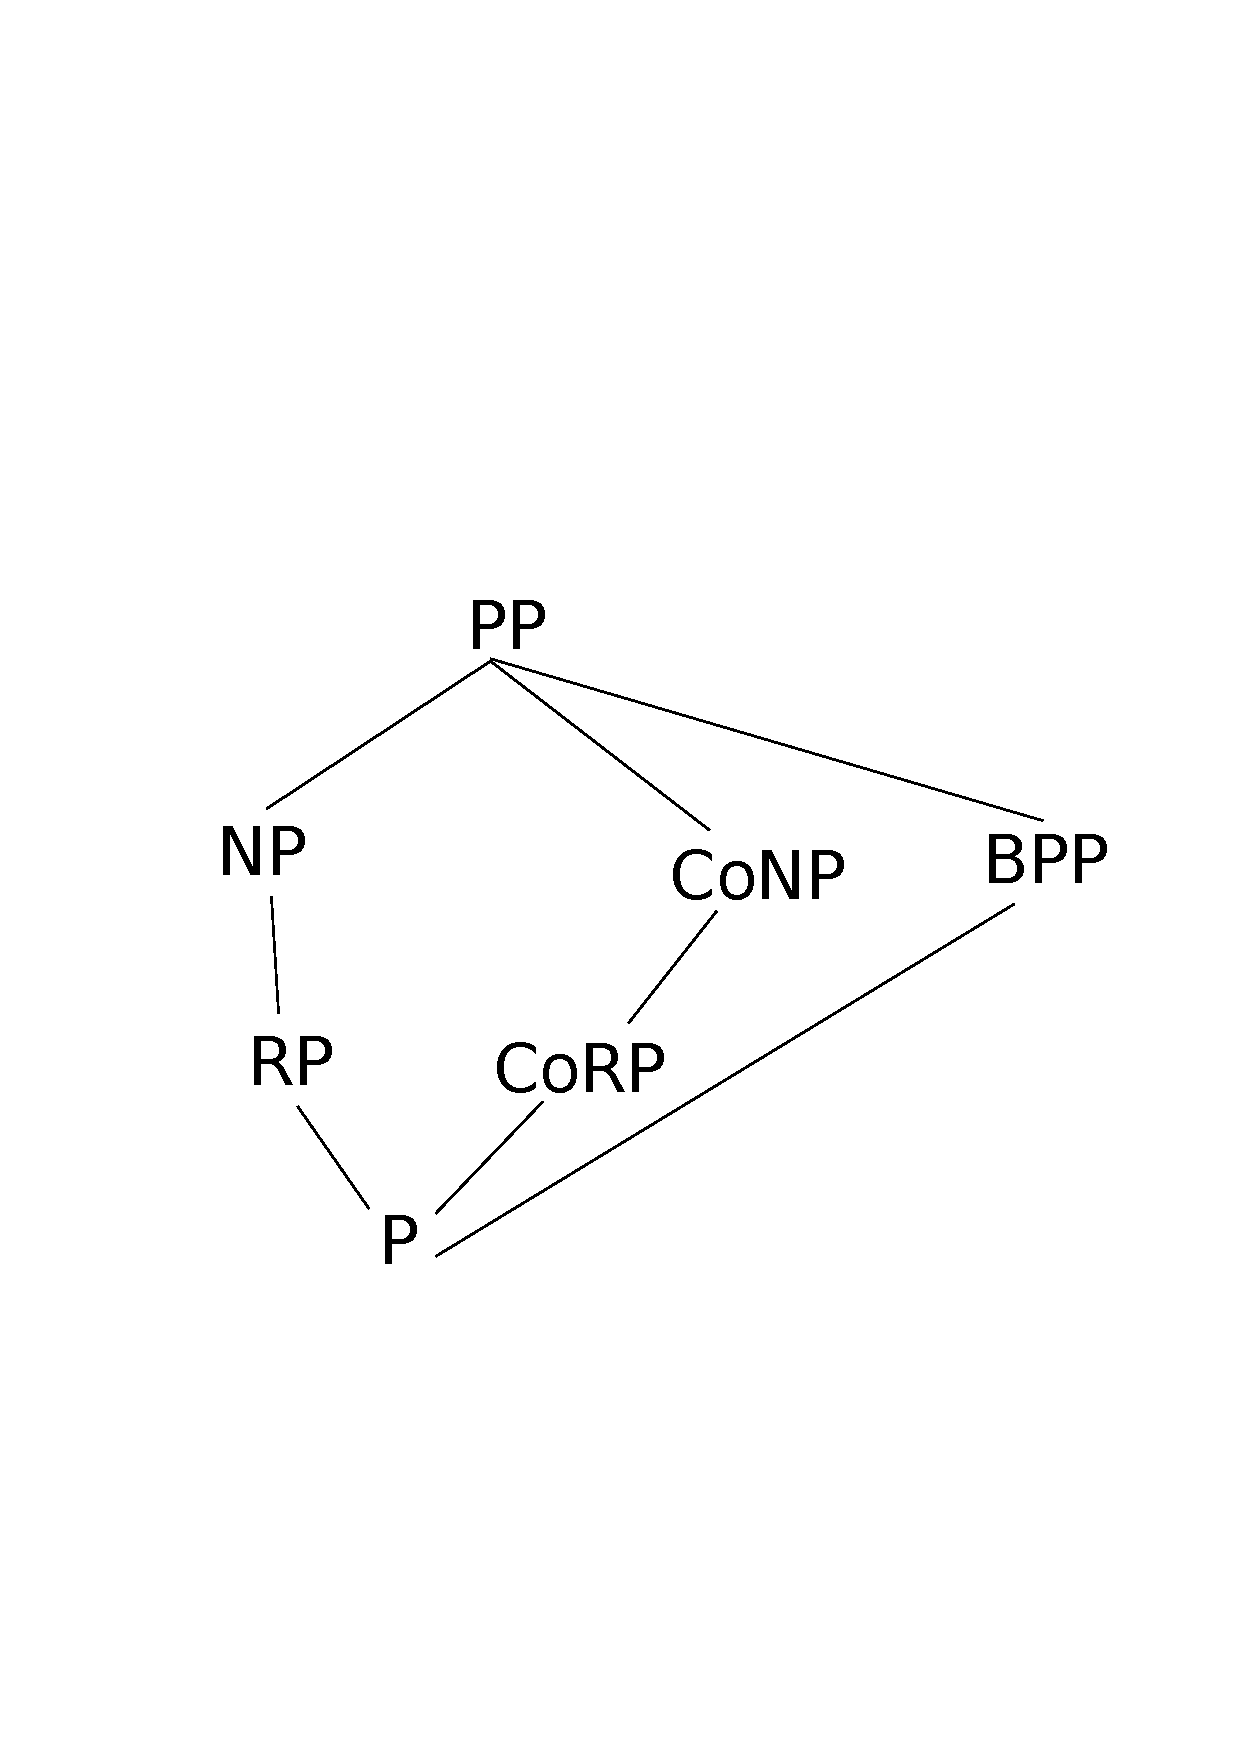
\includegraphics[scale=0.3, trim = 30mm 50mm 0mm 5mm, clip]{Lecture11-Princy/hie2}
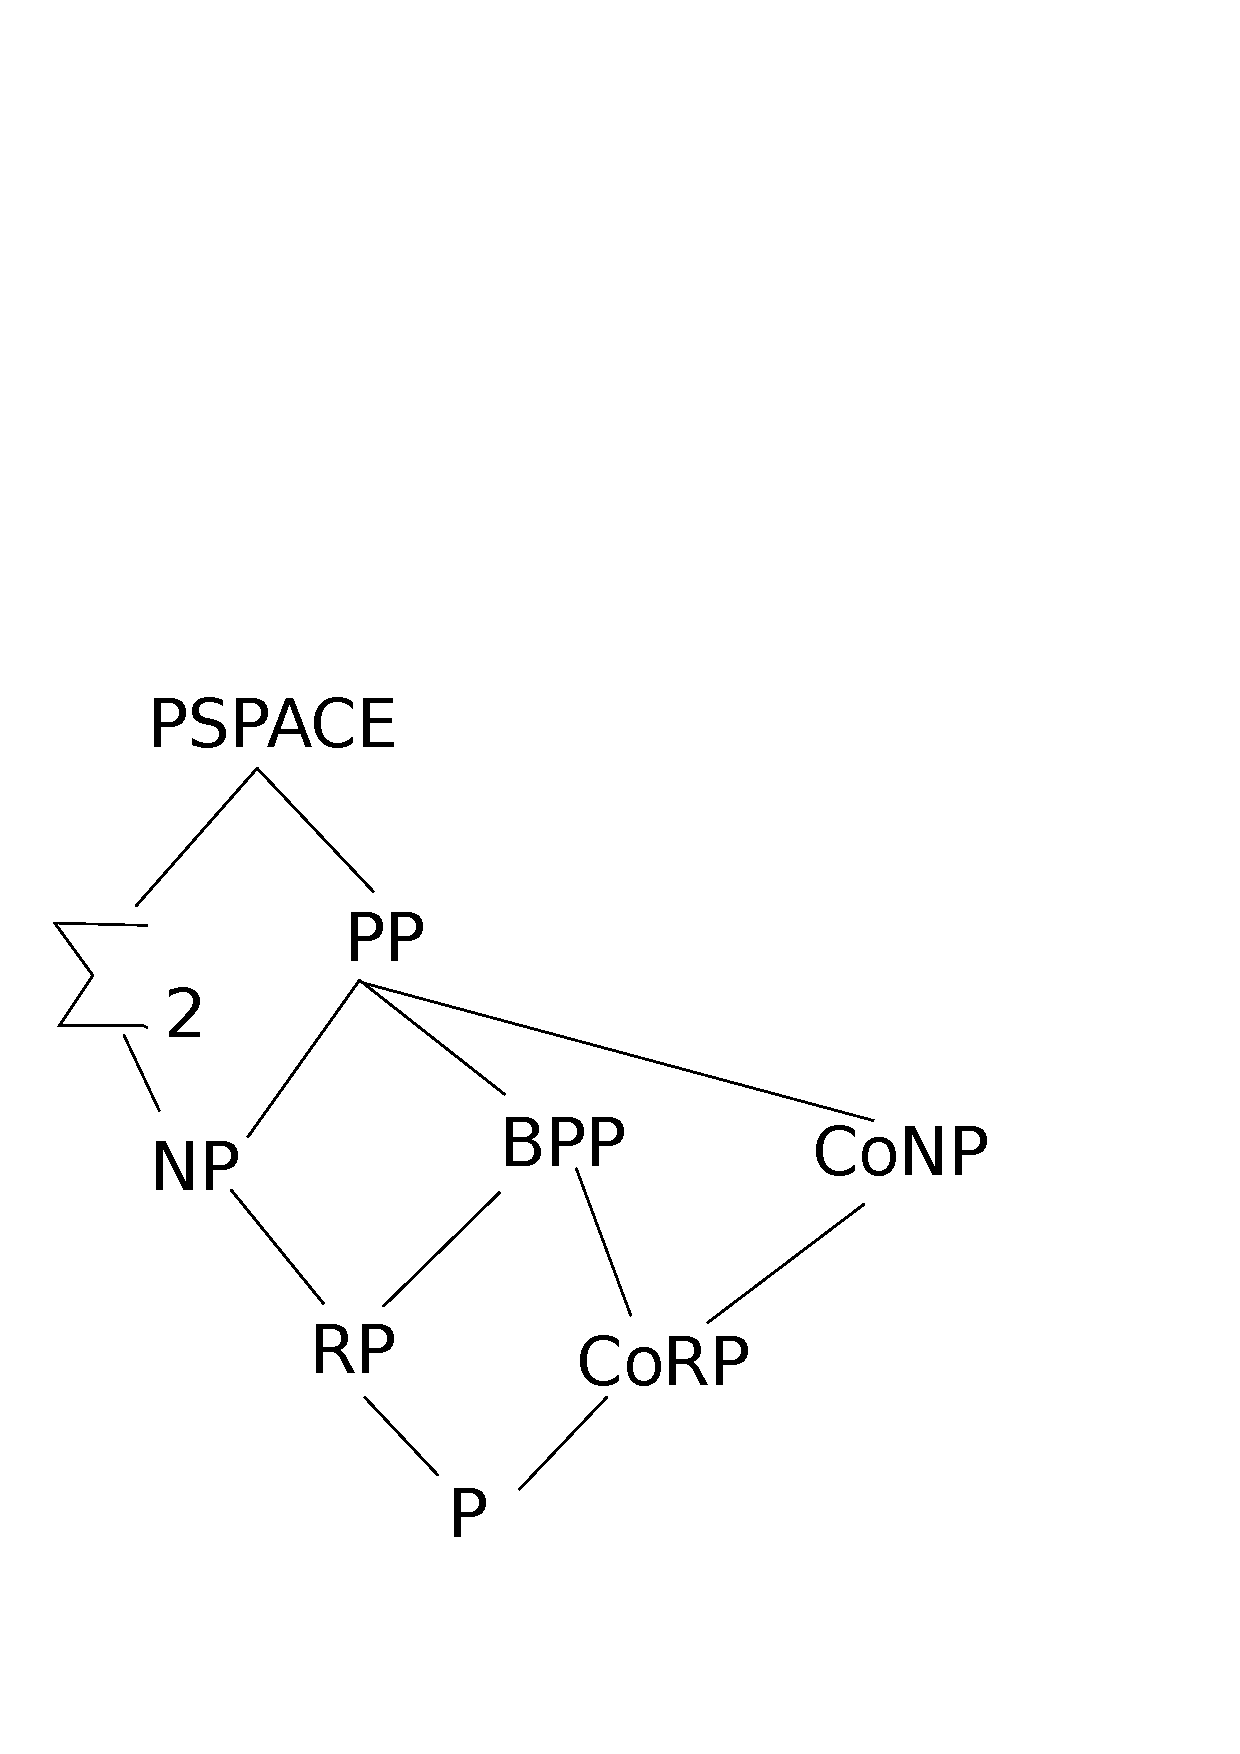
\includegraphics[scale=0.3]{Lecture11-Princy/hie3}
\end{center}
\vspace{-10mm}

\section{Derandomization of $\BPP$}
There are several questions connected to the new class $\BPP$ that contains several natural problems. We saw one example of multivariate polynomial identity testing problem. Is $BPP \subseteq P$? This would amount to showing that in the world of efficient computations, randomization does not add any power. There are reasons to remotely believe this to be the case, but till date there is no proof. 

A question of slightly different flavour is, if problems in $\BPP$ are contained in $\NP$? That is, can we trade non-determinism with randomness? We already know that if the randomness causes only one-sided error, then it can be replaced by simple non-deterministm ($\RP \subseteq \NP$). But extending this to two-sided error version is an interesting open problem in the area. 

We show a relaxed containment which can be seen to be an improved upper bound for problems in $\BPP$ compared to the trivial upper bound of $\PSPACE$.

\begin{theorem}
$BPP \in \Sigma_2$
\end{theorem}
\begin{proof}
Let $L \in \BPP$. By using amplification lemma for $q(n) = n$ we can state:
there is a probabilistic Turing machine $M$ and polynomial p(n) such that,
\[\#err_M(x) \leq 2^{-n} 2^{p(n)}\]

Let us recall the definition and a characterization of the class $\Sigma^2$
$\Sigma_2$ is defined as follows:
$L \in \Sigma_2$ iff $\exists B \in P $ such that:
\[x \in L \iff \exists y,  \forall z,  (x,y,z) \in B\]

There is a clear mindblock here. How do we tradeoff quantifiers to randomness?

Let us define a set A(x) as follows:
\[ A(x) = \{y\in \{0,1\}^{p(n)} |  M\ accepts\ x\ on\ path\ y \}\]

Observe that, 
\[x \in L \Rightarrow |A(x)| \geq (1- 2^{-n}) 2^{p(n)} \]
that is, no. of $y$'s such that $M(x,y) = 1$ is large.
\[x \notin L \Rightarrow |A(x)| \leq  2^{-n} 2^{p(n)}) \] 
that is, no, of $y$'s such that $M(x,y) = 1$ is small.
\\

\textbf{Parity Map:}
For two strings $y,z \in \{0,1\}^{p(n)}$, let $y \parity z$ denote the bit-wise parity of the two strings.
We can extend the parity map to operate on subsets of $\{0,1\}^{p(n)}$ as follows:
\[ S \parity z = \{y \parity z ~|~ y \in S \, z \in \{0,1\}^{p(n)} \}\]

\begin{observation}
For a fixed $z$, $\parity_z$ is a bijection from $\{0,1\}^{p(n)} \to \{0,1\}^{p(n)}$. That is, for any $z \in \{0,1\}^{p(n)}$, and $S \subseteq \{0,1\}^{p(n)}$, $|S| =|S \parity z|$.
\end{observation}

Ask the question : how many $z$'s do we need to cover $\{0,1\}^{p(n)}$ entirely?
That is, how large do we need $m$ to be, such that there exists strings $z_1, z_2, \ldots, z_m$ such that:
\[\bigcup_{i=1}^{m} (A(x) \parity z_i) = \{0,1\}^{p(n)}  \]

Intuitively, we expect the answer to be {\em small} when the size of $A(x)$ is large, and {\em large} when the size of $A(x)$ is small. Now we formalize this.

\textbf{Case 1:} Small $|A(x)| \leq 2^{-n} 2^{p(n)}$
In the best case, let each $z_i$ maps $A(x)$ to non-intersecting sets.
\[ \forall i, j (A(x)\parity z_i) \cap (A(x) \parity z_j) = \phi , i \neq j \]
\[|\bigcup_{i=1}^{m} (A(x) \parity z_i)| \geq |\{0,1\}^{p(n)}|\]
\[\Rightarrow m (2^{-n}) 2^{p(n)} \geq 2^{p(n)}\]
\[\Rightarrow m \geq 2^n\]

Hence, the no. of $z$'s required is exponential in $n$ when $A(x)$ is small, that is, when
$x \notin L$.
\\

\textbf{Case 2:} Large $|A(x)| \geq (1 - 2^{-n}) 2^{p(n)}$
We prove that $\exists z_1, z_2, z_3 ... z_m$ for a small $m$ such that 
\[|\bigcup_{i=1}^{m} (A(x) \parity z_i)| = |\{0,1\}^{p(n)}|\]
We call the $m$-tuple $z_1, z_2, z_3 ... z_m$ {\em bad}, if ,
\[|\bigcup_{i=1}^{m} (A(x) \parity z_i)| \neq |\{0,1\}^{p(n)}|\]
\[\Rightarrow \exists w \in \{0,1\}^{p(n)}, z_i \parity y \neq w ,\forall y \in
A(x), \forall i \]
\[\Rightarrow \{z_i \parity w | 1 \leq i \leq m \} \subset R(x)\]
where $R(x) = \bar A(x)$.
$|R(x)| = 2^{p(n)} - |A(x)|$
$\Rightarrow |R(x)| \leq  2^{p(n) - n}$

For a given $w$ and a given subset of $R(x)$ of size $m$, we get a {\em bad} $m$-tuple
$z_1, z_2, z_3 ... z_m$. Hence,
\\
Number of {\em bad} $z_1, z_2, z_3 ... z_m \leq $ Number of of $w$'s $\times$ Number of subsets
of $R(x)$ of size $m$.
\\
$\Rightarrow$ Number of {\em bad} $z_1, z_2, z_3 ... z_m \leq 2^{p(n)} (2 ^{p(n)-n})^m $
\\
Total number of $z_1, z_2, z_3 ... z_m $ = $(2^{p(n)})^m$.
$m$ should be such that,
\[2^{p(n)} (2 ^{p(n)-n})^m < (2^{p(n)})^m\]
\[p(n) + (p(n)-n)m < p(n)m\]
\[p(n) - nm < 0\]
\[m > \frac{p(n)}{n}\]

This goes well with our intuition. If $m$ is allowed to be very small, then we should not be able to cover the entire set $\{0,1\}^n$. For, $m > \frac{p(n)}{n}$ we are guaranteed to have atleast one {\em good} $m$-tuple, that is,
\[z_i \parity w = y , y \in A(x)\]

Hence we conclude that, 
\[\exists z_1, z_2, z_3 ... z_m , \forall w \in \{0,1\}^{p(n)} \left( \bigwedge_{i=1}^{m} \left[~z_i \parity w
\in A(x) ~\right] \right) \]
\[\exists z_1, z_2, z_3 ... z_m , \forall w \in \{0,1\}^{p(n)}, \left( \bigwedge_{i=1}^{m} \left[ ~M(x, z_i
\parity w) = 1 ~\right] \right) \]

Checking if $M$ accepts $x$ on a given path is a polynomial time operation, and
repeating it for each $z_i$ where the number of $z_i$'s is polynomial in $n$ is
also a polynomial time operation. Fix $m = p(n)$, Thus we have a $B \in \P$ such that

\[ x \in L \iff \exists \overline{z} \in \{0,1\}^{p(n)^2}, \forall w \in \{0,1\}^{p(n)} (x,\overline{z},w) \in B \]
Hence, the above language $L \in \Sigma_2$.
\end{proof}
  

\newpage \Lecture{Sajin Koroth}{January 28, 2012}{12}{One random string for all}
%\theme{Advice Classes and $\BPP$} 

%\lectureplan{

Today we will be
  showing an interesting consequence of amplification of $\BPP$
  introduced earlier. We will show that for an amplified $\BPP$
  algorithm there is a good string of random bits for each input
  length $n$ such that the algorithm run with these random bits is
  correct for all inputs $x$ of length $n$. Hence if you could get
  this good random string some how then you can decide a language in
  $\BPP$ in polynomial time without any randomness. But there is a
  catch, although we prove the existence of such a random string we do
  not know how to compute such a string efficiently. Hence we will
  introduce a new model of computation where you are given such advice
  strings for free, but the advice for all inputs of length $n$ has to
  be the same. We will introduce an advice string based class called
  $P/poly$, and will discuss its connection to $\BPP$
  %}

\section{One random string for all}
Recall that amplification allows to transform in polynomial time any
$\BPP$ algorithm to a $\BPP$ algorithm with error bound
$2^{-2n}$(i.e. at most $2^{-2n}$ fraction of random strings are ``bad'')
using $p(n)$ randomness. We will show that for a $\BPP$ algorithm with
the above mentioned error bound there is one random string for every
length $n$ such that for any input of that length $n$, the $\BPP$
algorithm outputs correctly on that random string. For the rest of the
lecture we will work with sufficiently amplified success probability
$\BPP$ machines, where the notion of sufficient success probability is
defined as given below :
\begin{align}
  x\in L \implies \Pr_{y} \left[ M(x,y) \text{ accepts } \right] & \geq
   1-2^{-2n} \\
  x \notin L \implies \Pr_{y}\left[ M(x,y) \text{ accepts } \right] & \geq
   2^{-2n} 
\end{align}
That is in such a machine the number of random strings $y$ which lead
the machine to output a wrong answer is bounded by $2^{-2n}$. Now let
us consider a matrix $A$ whose rows are indexed by inputs of length
$n$ and columns are indexed by random strings of length $p(n)$, and
the $(i,j)$th entry is $1$ if on fixing the random bits to be $j$ the
machine $M$ on input $i$ outputs correctly and it is $0$
otherwise. That is $A(i,j)=1$ if and only if $M(i,j)=\chi_L(i)$, where
$\chi_L(i)$ is the membership function of the language $L$
(i.e. $\chi_L(i)=1$ if and only if $i\in L$). By the amplification we
are guaranteed that for a given input $i$ at most $2^{-2n}$ fraction
of the random strings can have $A(i,j)=0$. Hence the total number of
zeros in the $A$ matrix is at most the number of rows times the
maximum number of zeros in a row, which is equal to 
\begin{eqnarray*}
  \text{\# 0's in matrix }A & \leq 2^n \times 2^{-2n} \times 2^{p(n)}
  \\
                            & \leq 2^{p(n)-n}
\end{eqnarray*}

But the total number of zeros, $2^{p(n)-n}$ is strictly less than the
number of columns in the matrix $A$. Hence there must be at least one
column with no zeros in it. If a column in the $A$ matrix has no zeros
then by the definition of $A$ matrix, the random string represented by
this column when fed as random bits to machine $M$ would output
correctly $\chi_L(x)$ for every $x\in \{0,1\}^{n}$.

\section{Class $\P/\poly$}

Even though we have proved the existence of a fixing of random bits
for an arbitrary input length $n$ of an amplified $\BPP$ machine $M$
such that the $M$ on these random bits decides all inputs $x$ of a
given length correctly for $L(M)$, we do not know how to compute such
a string efficiently (deterministically or using a randomized
algorithm) for arbitrary amplified $\BPP$ machines. Also note that the
good random string can vary with the input length. But if we can get
this random string for each input length $n$ for \textbf{free} then we
can decide a language in $\BPP$ in $\P$. That if there is a function
$h:N \to \{0,1\}^*$ such that $h(n)$ is at most polynomial in $n$ and
is the correct random string for the given $\BPP$ machine $M$, for all
inputs of length $n$, for all $n$ then we can construct a machine
$M^{'}$ such that it on input $(x,h(|x|))$ will simulate $M$ on $x$
using $h(|x|)$ as the random bits tape.

We will generalize the above ideas to define a class such that every
language in $\BPP$ is also in this class. 

\begin{definition}[$\P/\poly$]
A language $L$ is in $\P/\poly$ if there exists a polynomial $p(n)$, an
advice function $h:N\to \{0,1\}^*$ and a language $B\in \P$ such that
$\forall n,|h(n)|\leq p(n)$ and 
\begin{displaymath}
  x\in L  \iff (x,h(|x|)) \in B 
\end{displaymath}
where $|x|$ denotes the length of the string $x$.

\end{definition}

\subsection{$\BPP \subset \P/\poly$}

This is a straight forward corollary of the existence of a good random
string for any $\BPP$ machine, which works correctly for all inputs of
a given length. To show that for any $L\in \BPP$ it is also true that
$L\in \P/\poly$ we will use the fact that there a $\BPP$ machine $M_L$
accepting $L$ with error at most $2^{-2n}$ using at most $p(n)$ random
bits. We have already shown that for such a machine for every input
length $n$ at least one of $2^{p(n)}$ possible random strings is good
for all inputs of length $n$. We define the advice function $h(n)$ to
be a good random string which works for all inputs of length
$n$. Hence $|h(n)|=p(n)$ is at most polynomial in input length. Note
that definition of $P/poly$ doesn't have any requirements on the
computability of such a function, but needs the guarantee that such a
function exists. We will construct a machine $M_B$ running in
deterministic polynomial time which would accept
the language $B \in \P$ which accepts $(x,h(|x|))$ for all $x\in
L$. The machine $M_B$ on input $(x,h(|x|))$ starts simulating $M_L$ on
input $x$ using $h(|x|)$ as the random bits. By the definition of
$h(|x|)$, $M_L(x)$ using random bits $h(|x|)$ accepts if and only if
$x\in L$. Hence the proof.

\subsection{With advice comes the undecidable}

A consequence of the above definition of class $\P/\poly$ is that it not
only contains $BPP$, but it also contains some undecidable languages
as we do not insist on computability of advice function $h$. One such
undecidable language is \textbf{Unary Halting Problem} defined as 
\begin{displaymath}
  \text{UHP} = \left\{   1^n \mid \text{ Turing machine encoded by
      bin}(n) \text{ halts on all inputs}  \right\}
\end{displaymath}

It is easy to note that the general halting problem reduces to the unary
halting problem. Hence UHP is undecidable because HP is. 

We can also show that UHP is in $\P/\poly$. This is very straight
forward because the language is a unary language and there is exactly
one input of length $n$. Hence the advice function is simply a bit
representing the answer to the UHP on input $1^n$. Since we just need
a single bit of advice note that UHP is also in $\P/\theta(1)$. Also
from the above argument we can deduce that complement of UHP is also
in $\P/\poly$ because by modifying the $\P/\poly$ machine for UHP to
accept when $h(n)=0$ and reject otherwise where $h()$ is the advice
function for UHP, we get a $\P/\poly$ machine for
$\overline{\text{UHP}}$. Hence $\P/\poly$ not only contains complete
problems for semi-decidable languages, like UHP also contains
languages which are complete for co-semi-decidable languages, like
$\overline{\text{UHP}}$.



\newpage \Lecture{Sajin Koroth}{January 28, 2012}{13}{Self Reducibility of $\SAT$, Complete problem for  $\Sigma_k^\P$}
%\theme{Polynomial Hierarchy and its relation to $\P/\poly$}
%\lectureplan{
Recall that we introduced the advice based class $\P/\poly$
in the last lecture. We also saw that $\BPP \subsetneq \P/\poly$, and
by definition $\P \subsetneq \P/\poly$. But we don't know whether
$\NP\subsetneq \P/\poly$ or not. Hence if we could prove that $\NP
\not\subset \P/\poly$ then we would essentially be separating $\P$
from $\NP$. The reason why most of the complexity theorists believe $\NP
\not\subset \P/\poly$ is, if $\NP \subset \P/\poly$ then we would be
able to prove that $\PH=\Sigma_2^\P$, contrary to the common belief
that $\PH$ does not collapse. In today's lecture we will detail two
key ingredients needed for showing the above mentioned conditional
collapse of $\PH$, \textbf{a complete problem for $\Sigma_k^\P$} and
\textbf{self reducibility property of $\SAT$}
 % }

\section{Complete problem for the hierarchy}

We will first show a complete problem for the $k$th level of
polynomial hierarchy. Later on we will use the self-reducibility
nature of this problem to show the conditional collapse mentioned
earlier. Recall that a language $L$ is said to be in $\Sigma_k^\P$ 
if there exists polynomials $p_1,\dots,p_k$ and a machine $M$ running
in deterministic polynomial time such that
\begin{displaymath}
  x \in L \iff \exists y_1 \forall y_2 \exists y_3 \dots Q_k y_k
  \left[ M(x,y_1,y_2,y_3,\dots,y_k) = 1\right] , \forall i,|y_i|\leq p_i(|x|)
\end{displaymath}

Cook-Levin theorem guarantees that machine $M$ on input $x$ can be
converted into formula $\phi_x$ in polynomial time on variables
$y_1,y_2,\dots,y_k$ such that $\phi_x(y_1,y_2,y_3,\dots,y_k)$ is
satisfiable if and only if $M(x,y_1,y_2,y_3,\dots,y_k)$ accepts. Hence
we can say that the following problem is complete for $\Sigma_k^\P$,
\begin{definition}[$\Sigma_k-\SAT$] 
$\Sigma_k-\SAT$ is the set of all quantified Boolean formulas with at
most $k$ alternations (starting with an existential quantifier) which
are true. That is
\begin{displaymath}
  \Sigma_k-\SAT = \left\{ \exists y_1 \forall y_2 \exists y_3 \dots Q_k y_k
  \phi(y_1,\dots,y_k) \mid \exists y_1 \forall y_2 \exists y_3 \dots Q_k y_k
  \phi(y_1,\dots,y_k) \text{ is true} \right\}
\end{displaymath}
\end{definition}

The above problem is clearly in $\Sigma_k^\P$ as you can in polynomial
time construct from a formula, a machine in $\P$ for checking if the
formula is satisfiable or not given an assignment of all the variables
as input. The problem is $\Sigma_k^\P$ hard because
of Cook-Levin reduction from any machine in $\P$ to an equivalent formula.
 
\section{Self reducibility of $\SAT$}

Suppose we are given that $\NP \subset \P/\poly$ then we know that
there is a polynomial time deterministic Turing machine and a
polynomial length advice string for each input length such that the
machine decides a given language in $\NP$. We will sketch how this can
cause a collapse in the Polynomial Hierarchy, without giving the
details but exposing some difficulties which we have to overcome
before getting to the proof. To prove that $\PH$ collapses to
$\Sigma_2^\P$ it suffices to show that $\Sigma_3^\P=\Sigma_2^\P$. Recall
that $\Sigma_3^\P$ is the set of true quantified Boolean formulas which
are of the form $\exists y_1 \forall y_2 \exists y_3
M(x,y_1,y_2,y_3)$, and $\Sigma_2^\P$ are true quantified Boolean
formulas which are of the form $\exists y_1 \forall y_2
M(x,y_1,y_2)$. Also we are given that $\NP \subset \P/\poly$ hence for
any $L\in \NP$ there exists $h:N \to \{0,1\}^*$ and an $M\in \P$ such
that $x \in L$ if and only if $(x,h(|x|))$ is accepted by $M$. The
idea to place $\Sigma_3^\P$ in $\Sigma_2^\P$ is the following, the third
there exists $y_3$ and $M(x,y_1,y_2,y_3)$ can be combined to a machine
in $\NP$, where it first guesses a string $y_3$ of size $p_3(|y_3|)$
and then runs $M$ on $(x,y_1,y_2,y_3)$. We have assumed that
equivalent to this $\NP$ machine there is a $\P/\poly$ machine, and
even though we don't know the advice string we know there exists a
good advice string, and given the advice string the last ``there
exists'' quantifier in $\Sigma_3^\P$ can be eliminated by replacing it
with the polynomial time machine which is given the advice string,
hence we would a get a language in $\Sigma_2^\P$. But unfortunately we
don't know the advice string, hence the next best thing to do is to
guess the advice string using the first ``there exists'' quantifier in
$\Sigma_2^\P$. We are guaranteed that at least one guess is the
correct advice string. But there is a catch here, we could have
guessed the advice string incorrectly in some branch which in turn
could have led the machine $M$ to accept incorrectly thus falsely
accepting a string outside the language $L$ in $\Sigma_3^\P$. To get
around this problem we will use the first part to reduce the problem
in $\Sigma_3^\P$ to $\Sigma_3-\SAT$ and then use an algorithm for
$\SAT$ which given a sub-routine which tells a formula is satisfiable
or not, which uses a crucial property of the $\SAT$ problem,
self-reducibility to construct a satisfying assignment for the given
formula. And in the case it cannot construct a satisfying assignment
we would be able to guarantee that the advice string guessed is bad.

Self reducibility of $\SAT$ refers to the property of the $\SAT$
problem that checking a formula on $n$ variables is satisfiable
reduces to checking the satisfiability of two formulas on $n-1$
variables. This property leads to a polynomial time algorithm for
constructing a satisfying assignment given a polynomial time
sub-routine deciding the decision version of $\SAT$ problem
correctly. Algorithm~\ref{SAT_ASGN_ALGO} constructs a satisfying
assignment given a sub-routine which correctly solves $\SAT$ instances
of up to $n$ variables. Notice that one important property of
Algorithm~\ref{SAT_ASGN_ALGO} is that even if the sub-routine which
checks the satisfiability of a formula is wrong, the algorithm would
not be accepting an un-satisfiable formula as a satisfiable
formula. Because at the end of the algorithm we are checking whether
the assignment constructed by the algorithm is satisfiable or not, so
even if the sub-routine for $\SAT$, \textbf{SATISFIABLE} is
erroneous we would not be able to construct a satisfying assignment
for an un-satisfiable formula. But it might fail to construct a
satisfying assignment for a satisfiable formula if the sub-routine is
erroneous.

% Could not be added due to conflict with clrs package. Needs to be rewritten
% in algorithm 
%\begin{codebox}
%\label{SAT_ASGN_ALGO}
%  \Procname{$\proc{SATISFYING-ASSIGNMENT}(\phi(x_1,\dots,x_n))$}
%%  \li $\id{\psi(x_1,\dots,x_n)} \gets \phi(x_1,\dots,x_n)$
%  \li \For $i \gets 1$ \To $\id{n}$
%  \li \Do
%  \li $\id{\psi^{'}} \gets \psi(x_i=0)$
%  \li $\id{\psi^{''}} \gets \psi(x_i=1)$
%  \li \If $\proc(SATISFIABLE(\psi^{'}))$
%  \li \Then $\id{a_i} \gets 0$
%  \li       $\id{\psi} \gets \psi(0,x_2,\dots,x_n)$
%  \li \ElseIf $\proc(SATISFIABLE(\psi^{''}))$
%  \li \Then $\id{a_i} \gets 1$
%  \li       $\id{\psi} \gets \psi(1,x_2,\dots,x_n)$
%  \li \ElseNoIf
%  \li \Return $\const{impossible}$
%      \End
%  \li \If $\phi(a_1,\dots,a_n) = 1$ 
%  \li \Then \Return $(a_1,\dots,a_n)$
%  \li \Else \Return $\const{impossible}$
%      \End
%      \End
%\end{codebox}


\newpage \Lecture{Anup Joshi}{Jan 30, 2012}{14}{Karp-Lipton-Sipser Collapse Theorem}
%\theme{Between $\P$ and $\PSPACE$.}
%\lectureplan{ Karp-Lipton-Sipser Theorem : If $\NP$ is contained in $\P/\poly$ then $\PH$ collapses to
%$\Sigma_{2}$.}

We showed that $\BPP \subseteq \P/\poly$, and as we argued $\P/\poly$ seems to be a huge class containing $\P$ and $\BPP$, and even some undecidable languages. A natural question is whether $\NP$ is also contained in $\P/\poly$. We show that both answers to this question has interesting consequences.

Suppose we are able to prove that $\NP \not\subseteq \P/\poly$, then we are indeed are proving that $\NP \not\subseteq \P$. That is big !.

Suppose we are able to prove that $\NP \subseteq \P/\poly$. Does it have any consequences?
In this lecture, we will prove the Karp-Lipton-Sipser theorem, which says that if $\NP$ is
contained in $\P/poly$, then the polynomial hierarchy collapses to $\Sigma_{2}$. It is believed
that the polynomial hierarchy does not collapse, since the flavour of the question about each level of the hierarchy is about elimination of a quantifier, and is of a similar difficulty to to $\P$ vs $\NP$ question. 

Summarising this discussion; we believe that $\NP \not\subseteq \P$, but we do not know how to prove it. But then, since $\P \subseteq \P/\poly$ is this not a harder problem to solve that $\P vs \NP$? Yes, but why do we even bother to address it when we do not know how to attack the easier question? As we will see later in the course (when we do circuit complexity) this class $\P/\poly$ provides this nice escape from the "combinatorics of a Turing machine" and helps us to prove theorems which we do not know how to prove otherwise. It was for precisely this reason that, in the definition of $\P/\poly$ we did not make the advice function even computable (to avoid references to Turing machines).

We state the theorem.
\begin{theorem}[{\bf Karp-Lipton-Sipser, 1980}]
If $\NP \subseteq \P/\poly$, then $\PH$ collapses to $\Sigma_2$.
\end{theorem}

We prove the theorem by proving two lemmas. We first show that our assumption implies something much stronger. That is if $\NP \subseteq \P/\poly$ then not only $\NP$, but the entire $\PH$ will be in $\P/\poly$.

\begin{lemma}
 If $\NP \subseteq \P/\poly$, then $\PH \subseteq \P/\poly$.
\end{lemma}
\begin{proof}
It suffices to show that $\Sigma_{k} \subseteq \P/poly$ for any $k$. We prove this by induction on $k$.
For $k = 1$, it is trivially true, since $\Sigma_{1} = \NP$. Hence, the base case is true. Consider
an $L \in \Sigma_{2}$, then $L \in \NP^{B}$ for some $B \in \NP$. But $\NP \subseteq \P/poly$ (by
the induction hypothesis), hence, $\exists h : \mathbb{N} \rightarrow \{0, 1\}^*$ and $C \in P$,
such that, $y \in B \leftrightarrow  (y, h(y)) \in C$. Now, membership in $B$ is decidable in
polynomial time with the help of the advice function. Hence, we do not need to make oracle query to
$B$ to resolve membership questions in $L$, we can embed the polynomial time computation of the
oracle with advice function in the NTM for L itself. So we can say that, $L \in \NP$ with the advice
function $h : \mathbb{N} \rightarrow \{0, 1\}^*$. We can rewrite it as $\exists h : \mathbb{N}
\rightarrow \{0, 1\}^* \wedge C' \in \NP$ such that  $x \in L \leftrightarrow (x, h(|x|)) \in C'$.

Now, what can we say about $C'$? We know that $C' \in \NP$, hence $C' \in \P/poly$. Hence there is
an advice function for $C'$ also, so that membership in $C'$ is computable in polynomial time with
the help of that advice function. That is, $\exists g : \mathbb{N} \rightarrow \{0, 1\}^* \wedge D
\in \P$ such that  $y \in C' \leftrightarrow (y, g(|y|)) \in D$. Rewriting it we get:

\begin{center}
\begin{math}
 (x, h(|x|)) \in C' \leftrightarrow (x, h(|x|), g(p(x))) \in D
\end{math}
\end{center}

Hence from the above argument we see that $L \in \P/\poly$.
\end{proof}

Now we show that if any level of $\PH$ is in $\P\/poly$, then it essentially gives a way to express the acceptance condition using only two quantifiers. This is done in the following lemma.

\begin{lemma}
 For any $k > 2$, if $\Sigma_{k} \subseteq P/poly$, then $\Sigma_{k} \subseteq \Sigma_{2}$.
\end{lemma}
%\begin{proof-idea}
\begin{proof}
It suffices to show that $L \in \Sigma_{k} \implies L \in \Sigma_{2}$. For this, we take the
language $\SAT_{k}$ which is a quantified boolean formula with at most $k$ alternating
quantifiers. Since $\SAT_{k}$ is $\Sigma_{k}$-complete for any $k$, the lemma follows.

Let us assume that for any $k > 2$, $\Sigma_{k} \subseteq \P/\poly$. Let $L \in \Sigma_{k}$, and
since $\SAT_{k}$ is $\Sigma_{k}$-complete, then by our assumption, $\SAT_{k} \subseteq P/poly$. By
the definition of $\P/\poly$, $\exists h : \mathbb{N} \rightarrow \{0, 1\}^* \wedge B \in \P$ such that
$\phi \in \SAT_{k} \leftrightarrow (\phi, h(|\phi|)) \in B$. If $|\phi| = n$, then $h(n) \in \{0,
1\}^{p(n)}$. Let us define a new function $w$ in the following way:

\begin{center}
\begin{math}
 w = g(n) = (h(0), h(1), ..., h(n))
\end{math}
\end{center}
For any $\phi \in \Sigma_{k}$, such that $|\phi|
\leq n$, the string $w$ has the following properties:
\begin{enumerate}
\item $(0, w) \notin B$ $\wedge$ $(1, w) \in B$
\item If $\phi = \exists y, \psi \wedge \phi \in \SAT_{k}$, then $(\psi |_{y = 0}, w) \in B \vee
(\psi |_{y = 1}, w) \in B$.
\item If $\phi = \forall y, \psi \wedge \phi \in \SAT_{k}$, then $(\psi |_{y = 0}, w) \in B \wedge
(\psi |_{y = 1}, w) \in B$.
\end{enumerate}
Hence, $(\phi, w) \in B \implies 1, 2,$ and $3$ are satisfied.

It is also true in the other direction. That is, if $1, 2, $ and $3 $ are satisfied, then in order to check if $\phi$ is true, it suffices to check if $(\phi, w) \in B$. We can show this inductively. When $\phi$ is either $0$ or $1$, then by $1$, the above claim is true. Suppose, $\phi = (\exists x) \psi$, then we can apply $2$ on $\psi$ to evaluate it.
Otherwise, if $\phi = (\forall x) \psi$, then we can apply $3$ on $\psi$ to evaluate it. Thus, by recursively evaluating, we can reach upto the leaf where we apply $1$. Hence by a consistency check we can make sure that the advice does not give us a wrong answer, and indeed, if it gives a wrong answer to us, we can detect it at some point in the recursive evaluation. Note that we are using the self-reducibility property of $\SAT_k$ here.
Thus we have proved that,
\begin{center}
 \begin{math}
  \phi \in \SAT_{k} \leftrightarrow (\exists w, |w| \leq p(n)) (\forall \psi, |\psi| \leq n) (1
\wedge 2 \wedge 3 \wedge (\phi, w) \in B).
 \end{math}
\end{center}
\end{proof}


\newpage \newcommand{\USAT}{{\sf USAT}}
\Lecture{Nilkamal Adak}{Jan 31, 2012}{15}{Introduction to Toda's Theorem}
%\theme{Between $\P$ and $\PSPACE$.}
%\lectureplan{Introduce Toda's Theorem, give some relevant definitions 
%and construct a proof strategy for Toda's Theorem}

There are two different way to generalize hard problems like optimization 
problems.
\begin{enumerate}
 \item Non-determinism or quantification
 \item Counting
\end{enumerate}

It was an important open question in 1980's about relative power of those 
two approach, alternation and counting. There are various 
classes are defined independently in those two different approach. But how 
are those class comparable? In 1991, Toda came up with the following relation 
among the two different world.

\begin{theorem}
 $PH \subseteq \P^{\#\P}$
\end{theorem}
This theorem take the whole quantification world to counting world. That is 
we can solve any problem in PH in polynomial with an oracle access to 
a $\#\P$-Complete problem. Before going to the proof of Toda's theorem lets 
define the following.

\begin{definition}
$\exists.$ Operator.

Let us consider the definition of $\NP$.
\begin{center}
$L \in \NP$ if $ \exists B \in \P$ such that 
\[ x \in L \Longleftrightarrow \exists y \text{ such that } (x,y) \in B \]
\end{center}
\end{definition}
So we can think $\exists$ as an operator and let us define it as follows

Let $C$ be any class of languages. Define, 
\begin{center}
$ L \in \exists.C$  if $\exists B \in C$  such that
$x \in L \Longleftrightarrow \exists y$ such that $(x,y) \in B$
\end{center}
So $\NP = \exists .\P$

\begin{definition}
BP. Operator \\
Let us consider definition of the class $\BPP$ 

$L \in \BPP$ if $\exists B \in \P$ such that 
\begin{align*}
x \in L & \Longrightarrow {\sf Pr_y}[(x,y) \in B ] \ge \frac{3}{4} \\
x \notin L & \Longrightarrow {\sf Pr_y}[(x,y) \in B] \le \frac{1}{4}
\end{align*}
So similarly we can define BP. operator as 


\begin{center}
Let $C$ be a class of languages. 
$L \in BP.C$ if $ \exists B \in$ C such that
\begin{align*}
x \in L & \Longrightarrow {\sf Pr}[(x,y) \in B]  \ge \frac{3}{4}\\
x \notin L & \Longrightarrow {\sf Pr}[(x,y) \in B] \le \frac{1}{4}
\end{align*}
\end{center}
So $\BPP = BP.\P$
\end{definition}

Now lets define the class $\oplus \P$:
\begin{definition}
L $\in \oplus \P$ if there is a branching machine $M$ such that
\[ x \in L \Longrightarrow \#Acc_M(x) \text{ is odd} \]
\end{definition}

$\oplus\P$ can be considered as the class of decision problems corresponding 
to the least significant bit of a $\#\P$-problem. Now the natural 
question is ``Is $\NP \subseteq \oplus\P$?''.

We will see that $NP$ problems are reduced to $\oplus\P$ in some extend.
Lets now define Randomize Reduction as follows
\begin{definition}
$A \le B$ via a randomize reduction function $\sigma$ if 
\begin{enumerate}
\item  $\sigma$ is computable by choosing a random string 
$y \in \{0,1\}^{p(n)}$.
\item $x \in L \iff \sigma_y(x) \in B$ with high probability.
\end{enumerate}
\end{definition}

We will see that $\NP$ problems are reduced to some $\oplus\P$ problem 
via randomize reduction. More specifically $\NP \subseteq BP.(\oplus \P)$.
Now we will develop the proof strategy for Toda's theorem. 
We will proof the theorem in the following steps $\ldots$ 
\[
\NP \subseteq BP.(\oplus \P) \subseteq \BPP^{\oplus \P} \subseteq 
\P^{\#\P}=\P^{\PP} \]
Then by induction on the number of quantifiers we will show that the 
entire $PH \subseteq \P^{\#\P}$.

So our first step is to show $\NP \subseteq BP.(\oplus \P)$.

To prove this claim let us define the following languages \ldots.
\begin{definition} 
\[ \oplus \SAT = \{ \phi : \# \text{ of satisfying assignment of }
\phi \text{ is odd} \}\]
\end{definition}

Let us define the following promise problem \USAT as,
\begin{definition}
For all boolean formulas $\phi$,
\begin{align*}
\phi & \in \USAT \Longrightarrow \#SAT(\phi)=1\\
\phi & \notin \USAT \Longrightarrow \#SAT(\phi)=0
\end{align*}
\end{definition}

This is a promise problem as we will consider only those $\phi$ which 
falls into above two cases. Now we introduce a very important result called 
\emph{Valiant-Vazirani lemma} proved by Valiant and Vazirani in 1986.

\begin{lemma}(Valiant-Vazirani Lemma) \\
There exists a randomize reduction $\sigma_y$ such that
\begin{align*}
\phi & \in \SAT \iff Pr_y[\sigma_y(\phi) \in \USAT] \ge \frac{3}{4}\\
\phi & \notin \SAT \iff Pr_y[\sigma_y(\phi) \in \USAT] \le \frac{1}{4}
\end{align*}
\end{lemma}
We will prove this lemma in the next lecture and using this lemma 
we will prove our first step $\NP \subseteq BP.(\oplus\P)$.

\newpage \Lecture{Rahul CS, Karthik Abhinav}{Feb 2, 2012}{16}{Valiant-Vazirani Lemma}
%\theme{NP $\subseteq$ BP.($\oplus$P)}
%\lectureplan{Randomized Reduction from SAT to $\oplus$SAT}

%SAT $\leq^{m}_{r}$ $\oplus$ SAT

In the last lecture, we outlined an approach to prove Toda's theorem. One of the key ingredients was a partial answer to the question that we had in one of the earlier lectures. Is $\NP$ contained in $\oplus\P$? In the last lecture we viewed $\exists$, $\oplus$, $\BP$ as operators on complexity classes and stated that $\NP$ is contained in $\BP.(\oplus\P)$. 
We also interpreted this in the following way; there is a randomized reduction from $\SAT$ to a language in $\oplus\P$.

\section{Randomized Reduction from SAT to $\oplus$SAT}
Define languages, 
\begin{itemize}
\item[]USAT=$\{\phi \mid \#\phi=1\}$ \newline where $\#\phi$ is the number of satisfying assignments to the formula $\phi$
\item[]$\oplus$SAT=$\{\phi \mid \exists k \in \mathbb{N}, \#\phi=2k+1\}$
\end{itemize}

The following Lemma, famously known as the Valiant-Vazirani Lemma, was proved by Valiant and Vazirani in 1986. It proved instrumental for many results later, including Toda's theorem which we will be taking up in the next lecture.

The lemma states the following reduction from $\SAT$ to $USAT$. 

\begin{lemma}[{\bf Valiant-Vazirani Lemma}]
There exists a randomized polynomial time algorithm that takes input $\phi$ and produces a formula $\psi_{\phi,y}$ (say $\psi$) such that,
\begin{eqnarray*}
\phi \in \SAT \implies Pr(\psi \in USAT) & \geq & \frac{1}{8n} \\
\phi \not\in \SAT \implies Pr (\psi' \not\in USAT) & = & 1
\end{eqnarray*}
\end{lemma}

Clearly, $\psi \in$ USAT $\Rightarrow \psi \in \oplus$ SAT. In the other case since $\psi \notin \SAT$, it is also case that $\psi \notin \oplus\SAT$. Thus as a corollary to the lemma, we get:

\begin{corollary}
There exists a randomized polynomial time algorithm that takes input $\phi$ and produces a formula $\psi$ such that,
\begin{eqnarray*}
\phi \in \SAT \implies Pr(\psi \in \oplus\SAT) & \geq &  \frac{1}{8n} \\
\phi \not\in \SAT \implies Pr (\psi \not\in \oplus\SAT) & = & 1
\end{eqnarray*}
\end{corollary}

\begin{proof}
We present a high-level idea first. Given $\phi$, a natural approach to produce a formula with unique satisfying assignment is to add another conjunction to produce $\psi = \phi \land (\omega)$ such that $\omega$ 
filters out the satisfying assignments using the clause $\omega$ such that only one of them will satisfy the resulting formula. Clearly, if $\phi$ is not satisfiable, then by construction, $\psi$ is also not satisfiable, no matter what $\omega$ is. Consider the case when $\phi$ is satisfiable. Thus, we want $\omega$ to state a property which only one of the satisfying assignments have. 

We use hashing to achieve this. That is, we will make $\omega$ state that $h(x) = 0^k$ where $0^k$ is in range of the hash family and $x$ is an assignment. The probability that there is a collision at $0^k$ for two $x$s that satisfy $\phi$ (that is, probability that two assignments that satisfy $\phi$ also satisfies $\omega$) can be controlled by choosing a nice hash family. Thus our filter, with high probability, filters out a unique satisfying assignment for $\psi$ from the set of satisfying assignments of $\phi$.

Usually, we design hash families with a size parameter $k$; the size up to which we want to guarantee collision-free property. But here we do not know the size of the subset (the set of satisfying assignments) a priori for which we are trying to achieve unique mapping(collision-free). The smaller the subset the smaller the range (of the hash functions) that we can work with. Let us say we choose randomly the number $k$ such that the number of satisfying assignments is between $2^k$ and $2^{k+1}$ and then decide hash function for all subsets of that size. Since the number of satisfying assignments could be any number from $0$ to $2^n$, we have already lost out a bit on the probability but by a factor of at most $\frac{1}{n}$.

Now we will formally address this intuition.
Let $T \subseteq \{0,1\}^n$ be the set of satisfying assignments of $\phi$. Select $k \in \{0,1,...,n-1\}$ such that $2^k \leq |T| \leq 2^{k+1}$. Let $H_{n,k}$ be a collection of functions $h: \{0,1\}^n \mapsto \{0,1\}^k$. $H_{n,k}$ is said to be pairwise independent if for every $x$,$x' \in \{0,1\}^n$ with $x \neq x'$ and for every $y$,$y' \in \{0, 1\}^k$, 
\[ \underset{h \in_R H_{n,k}}{Pr}[h(x) = y \wedge h(x') =y'] = \frac{1}{2^k}.\frac{1}{2^k}=2^{ -2k}
\]
Construct a family of pairwise independent hash functions $H_{n,k+2}$. Hence, 
\[
\stackrel{Pr}{_{h \in H,x \in T}}[h(x)=0^{k+2}]=\frac{1}{2^{k+2}}
\]

We calculate the probability of existence of a hash function $h \in H$ such that $h$ maps exactly one satisfying assignment $x \in T$ to 0$^{k+2}$. This parameter is given by,
\[
\stackrel{Pr}{_{h \in H}}[|\{x \mid x \in T, h(x)=0^{k+2}\}|=1]
\]

Once we have an $h$ satisfying the above condition, the number of satisfying assignments for $\phi$ will be exactly 1. That is, in the described transformation, if $\omega$ is $h(x)=0^{k+2}$, the number of satisfying assignments for $\psi$ will be exactly 1, if it is satisfiable. Note that we can consider the computation sequence of the hash function $h$ on a turing machine and convert that to a SAT formula using Cook-Levin reduction. We claim that,  
\[
\stackrel{Pr}{_{_{_{h \in H}}}}[|\{x \mid x \in T, h(x)=0^{k+2}\}|=1] \geq \frac{1}{8}
\]
Consider, 
\begin{eqnarray*}
\stackrel{Pr}{_{_{_{h \in H}}}}[\exists x \in T, h(x)=0^{k+2} \wedge \underset{x' \in T,x' \neq x}\forall h(x') \neq 
0^{k+2}] & & \\
\end{eqnarray*}

\begin{eqnarray*}
= & \stackrel{Pr}{_{_{_{h}}}}[\underset{x' \in T,x' \neq x}\forall h(x') \neq 0^{k+2} \mid h(x)=0^{k+2}].\stackrel{Pr}{_{_{_{h}}}}[h(x)=0^{k+2}] & \\
= & (1-\stackrel{Pr}{_{_{_{h}}}}[\underset{x' \in T,x' \neq x}\exists h(x') = 0^{k+2}|h(x)=0^{k+2}]).\stackrel{Pr}{_{_{_{h}}}}[h(x)=0^{k+2}] & \\
= & (1-\stackrel{\sum}{_{_{_{_{\stackrel{x' \in T}{x' \neq x}}}}}}\stackrel{Pr}{_{_{_{h}}}}[h(x')=0^{k+2}\mid h(x)=0^{k+2}]).\stackrel{Pr}{_{_{_{h}}}}[h(x)=0^{k+2}] & \\
\end{eqnarray*}

Let us calculate the first part of the expression, $(1-\stackrel{\sum}{_{_{_{_{\stackrel{x' \in T}{x' \neq x}}}}}}\stackrel{Pr}{_{_{_{h}}}}[h(x')=0^{k+2} \mid h(x)=0^{k+2}])$. Since $h$ is sampled from a family of pairwise independent hash functions, $h$ satisfies the condition of simple uniform hashing. That is, the events $h(x)=0^{k+2}$ and $h(x')=0^{k+2}$ are independent. Therefore,
\[
\stackrel{\sum}{_{_{_{_{\stackrel{x' \in T}{x' \neq x}}}}}}\stackrel{Pr}{_{_{_{h}}}}[h(x')=0^{k+2} \mid h(x)=0^{k+2}])=\stackrel{\sum}{_{_{_{_{\stackrel{x' \in T}{x' \neq x}}}}}}\frac{1}{2^{k+2}}= |T-\{x\}|.\frac{1}{2^{k+2}}
\]
We bound the expression from above by bounding $|T-\{x\}|$ from above. That is,
\[
\stackrel{\sum}{_{_{_{_{\stackrel{x' \in T}{x' \neq x}}}}}}\stackrel{Pr}{_{_{_{h}}}}[h(x')=0^{k+2}\mid h(x)=0^{k+2}]) \leq (2^{k+1}-1) \frac{1}{2^{k+2}}
\]
Hence, 
\begin{eqnarray*}
(1-\stackrel{\sum}{_{_{_{_{\stackrel{x' \in T}{x' \neq x}}}}}}\stackrel{Pr}{_{_{_{h}}}}[h(x')=0^{k+2}\mid h(x)=0^{k+2}]) 
& \geq & 1-(2^{k+1}-1)\frac{1}{2^{k+2}} \\
& = & 1-\frac{1}{2}[\frac{(2^{k+1}-1)}{2^{k+2}}] \\
& \geq & \frac{1}{2}
\end{eqnarray*}
Therefore, 
\[
(1-\stackrel{\sum}{_{_{_{_{\stackrel{x' \in T}{x' \neq x}}}}}}\stackrel{Pr}{_{_{_{h}}}}[h(x')=0^{k+2}|h(x)=0^{k+2}]).\stackrel{Pr}{_{_{_{h}}}}[h(x)=0^{k+2}]\geq \frac{1}{2}\cdot \frac{1}{2^{k+2}}
\]

Thus, 
\[
|T|.(1-\stackrel{\sum}{_{_{_{_{\stackrel{x' \in T}{x' \neq x}}}}}}\stackrel{Pr}{_{_{_{h}}}}[h(x')=0^{k+2}\mid h(x)=0^{k+2}]).\stackrel{Pr}{_{_{_{h}}}}[h(x)=0^{k+2}] \geq  |T|.\frac{1}{2}\frac{1}{2^{k+2}} 
\]
By bounding $|T|$ from below, the probability that there is a $x \in T$ which uniquely gets mapped to $0^{k+2}$ is given by,
\[
|T|.(1-\stackrel{\sum}{_{_{_{_{\stackrel{x' \in T}{x' \neq x}}}}}}\stackrel{Pr}{_{_{_{h}}}}[h(x')=0^{k+2}\mid h(x)=0^{k+2}]).\stackrel{Pr}{_{_{_{h}}}}[h(x)=0^{k+2}]\geq\frac{1}{2^{k}}\frac{1}{2}\frac{1}{2^{k+2}} \geq \frac{1}{8}
\]

Considering the fact that $k \in \{0,1,...,n-1\}$ satisfies $2^k \leq |T| \leq 2^{k+1}$ with probability $\frac{1}{n}$ we get,
\[
\phi \in \SAT \implies \stackrel{Pr}{_{_{_{x}}}}[\psi_{\phi,x} \in USAT] \geq \frac{1}{8n}
\]
\[
\phi \not\in \SAT \implies \stackrel{Pr}{_{_{_{x}}}}[\psi_{\phi,x} \not\in USAT] = 1
\]
\end{proof}

Now we make comments about amplification of success probability. Since the algorithm is one-sided error, an approach will be to simply repeat the experiment some $\ell$ times, and take the $\lor$ of the results. This however, causes loss of uniqueness of the assignment since different $h$ may make different $x$s to go to $0^k$. However, we can still preserve the parity with high probability that results in the following amplification result which we state as a Lemma.

\begin{lemma}
There exists a randomized polynomial time algorithm that takes input $\phi$ and produces a formula $\psi'$ such that,
\begin{eqnarray*}
\phi \in \SAT \implies Pr(\psi' \in \oplus\SAT) & \geq & 1-\frac{1}{2^{q(n)}} \\
\phi \not\in \SAT \implies Pr (\psi' \not\in \oplus\SAT] & = & 1
\end{eqnarray*}
\end{lemma}

The OR amplification says, that we report that $\phi \in \oplus\SAT$ if and only if at least one of the trials produces a formula in $\oplus\SAT$. But then, can we produce a single formula $\psi'$ such that if $\phi$ is in $\SAT$, then $\psi'$ is in $\oplus\SAT$ with high probability. We will address such a reduction in the next lecture.


Note that it is an open problem to boost the probability of $\frac{1}{8n}$ in the Valiant-Vazirani reduction to USAT.%\textbf{Attempt to Amplify:}

\newpage \Lecture{Princy Lunawat, Karthik Abhinav}{Feb 6, 2012}{17}{Reductions to $\oplus$-\SAT : Amplified version}
%\theme{}
%\lectureplan{}

The last few lectures focus on the Toda's theorem which states
that $\PH \subseteq \P^{\#\P}$. The first half of the proof of the theorem
shows a randomized reduction from $\PH$ to $\parity \SAT$. 

We proved the Valiant-Vazirani lemma which stated a randomized polynomial time algorithm that takes in a formula $\phi$ and produces a new formula $\psi$ such that it gives a {\em weak form} of a randomized reduction from $\SAT$ to $U\SAT$.  We have the following 
\begin{eqnarray*}
\phi \in \SAT & \implies & Pr \left( \psi \in \textrm{\sc U\SAT} \right) \ge \frac{1}{8n} \\
\phi \notin \SAT & \implies & Pr \left( \psi \notin {\sc U\SAT} \right) = 1
\end{eqnarray*}

We also concluded that this gives a weak\footnote{The reduction is weak because the error probability($1-\frac{1}{8n}$) is much more than what is allowed in a randomized reduction ($\frac{1}{2}$)} randomized reduction from $\NP$ to $\parity\SAT$.  Now we show how to amplify the success probability in the case of the reduction to $\parity \SAT$. \footnote{Such an amplification is not known for the case of $U\SAT$.}

Indeed, something special about $\parity$ is going to help us. In this lecture, we explore some properties of the $\parity$ quantifier which are used to come up with a formula $\phi''$ from a given formula $\phi \in \SAT $ such that $\phi'' \in \parity \SAT$ with high probability. We thereby deduce that $\NP <^m_r \parity \SAT$.

\section{Parity Addition, Complementation and Multiplication}
Given two boolean formulae, $\phi $ and $\phi'$, their parity can be added as follows: 
\[\parity(\phi + \phi')(\bar z) = \parity(z_0 = 0 \wedge \phi) \vee \parity(z_1 = 0 \wedge \phi')  \]
Similarly, the parity can be complemented as: 
\[(z= 0 )\wedge (\sim x_1 \wedge \sim x_2 \wedge \ldots \wedge \sim x_n ) \vee (\phi \wedge z = 1)\]
which is represented as $\phi + 1$.
Multiplication of parity is obtained as: 
\[\parity \phi(\bar z) \times \parity \phi'(\bar z) = \parity (\phi(\bar z) \wedge \phi'(\bar z)) \]
\section{Randomized Reduction}

	In our construction for the Valiant-Vazirani Lemma , we defined a formula $\psi_i = \phi \wedge (h_i(x)= 0^k)$
where $x$ is an assignment of $\phi$.Now consider a formula $\phi' = \overset{l-1}{\underset{i = 0} \wedge } (\parity
\psi_i)$. if Pr$\left[\psi_i \in \texttt{USAT} \right] \geq \frac{1}{8n}$, then Pr$\left[ \phi' \in \SAT\right] = 1 -
\left(1 - \frac{1}{8n } \right)^l]$. We now come up with a formula $\phi''$ equivalent to $\phi'$ such that the parity
of $\phi''$  is odd. that is, $\phi'' \in \parity \SAT$ conditioned on the probability that atleast one $\psi_i \in
\parity \SAT $.\\
For simplicity, consider $\psi_1$ and $\psi_2$, one of which is in $\parity \SAT$.We observe that both ,
$\psi_1 + 1$ and $\psi_2 + 1$ cannot have an odd parity. Therefore,we have, 
\begin{align*}
\parity(\psi_1 + 1) .(\psi_2 + 1) =& 0\\
\parity((\psi_1 + 1) .(\psi_2 + 1)+ 1) =& 1 
\end{align*}
Hence, $((\psi_1 + 1) .(\psi_2 + 1)+ 1) \in \parity \SAT$.In general , 
$\overset{l-1}{ \underset{i = 0}\wedge} ((\psi_i + 1)+ 1) \in \parity \SAT$ which is our new formula $\phi''$
equivalent to $\phi.$ Hence , Pr$\left[\phi'' \in \parity \SAT \right]$ is the same as that of atleast one $\psi_i$
having an odd parity.
 \[\phi \in \SAT \Rightarrow Pr \left[\phi'' \in \parity \SAT \right] =1 -\left(1 - \frac{1}{8n }\right)^l \]

To amplify this probabilty to $1 - 2^{-m} $ we choose an appropriate value of $l$ such that,
\[1 -\left(1 - \frac{1}{8n }\right)^l \geq 1 - 2^{-m} \]

Hence, we have 
\begin{eqnarray*}
 \phi \in \SAT & \Rightarrow &  Pr\left[\phi'' \in \parity \SAT \right]\geq  1 - 2^{-m} \\
 \phi \notin \SAT & \Rightarrow & Pr\left[\phi'' \in \parity \SAT \right] = 0 
\end{eqnarray*}

Hence, $\NP <^m_r \parity \SAT$.
 


\newpage \Lecture{Sunil K.S., Karthik Abhinav}{Feb 07, 2012}{18}{Proof of Toda's Theorem}
%\theme{Between P and PSPACE}
%\lectureplan{In this lecture we will be concluding the lectures on the
%  theme of contrasting the power of counting to that of
%  alternations. Today we will be proving the interesting result that
%  $\PH \subseteq \P^{\#\P}$. To do this, first using the
%  Valiant-Vazirani lemma we will show that $\PH \subseteq
%  \BP(\parity\P)$.}
\section{Valiant-Vazirani Lemma}
We have already saw Valiant-Vazirani theorem which stated that :
\begin{lemma} Valiant-Vazirani Theorem: There exists a probabilistic
polynomial-time algorithm f such that for every n-variable boolean
formula $\varphi$
\begin{eqnarray*}
  \varphi\in SAT\Rightarrow Pr[f(\chi)\in \parity SAT] &\geq& \frac{1}{8n} \\
  \varphi\notin SAT\Rightarrow Pr[f(\chi)\in \parity SAT] &=& 0
\end{eqnarray*}
\end{lemma}
But to prove that $\PH \subseteq \BP(\parity\P)$ we will need
amplified version of this lemma.
\begin{lemma}
Valiant-Vazirani lemma (Amplified version): There exists a randomized
algorithm which produce $\varphi$ from a given boolean formula $\phi$
such that for a polynomial $q(n)$:
\begin{eqnarray*}
  x\in L \Rightarrow Pr[\varphi\in \parity SAT] &\geq&
  \left(1-\frac{1}{2^{q(n)}}\right) \\ 
  x\notin L \Rightarrow Pr[\varphi\in \parity SAT] &\leq& \left(\frac{1}{2^{q(n)}}\right)
\end{eqnarray*}
\end{lemma}

\section{Toda's Theorem: $\PH\subseteq\P^{\#\P}$} Any problem in $\PH$
can be solved by a $\P$ machine by making queries to a $\#\P$ oracle.\newline

\textbf{Proof} \newline
This theorem will be proved in two parts
\begin{itemize}
 \item 
 $\PH\subseteq\BP(\parity\P)$
 \item
 $\BP(\parity\P) \subseteq \P^{\#P}$
\end{itemize}

% This part has been untouched. Should be modified
\textbf{Claim}: $\PH\subseteq\BP(\parity\P)$
\begin{proof} Proof by induction on the number of alterations, $k$.\\
  Basis: for $k=0$, we already have the result
  $\NP\subseteq\BP(\parity\P)$.\\ Assume the result for $k$. ie;
  $\Sigma_k$ or $SAT_k$ $\in \BP(\parity\P)$.\\ We need to prove that
  $SAT_{k+1}\in \BP(\parity\P)$.

  Consider a language L $\in \Sigma_{k+1}^{p}$, 
  $$ x \in L \Leftrightarrow \exists y_{1} \forall y_{2} (y_{1},y_{2}) \in B$$ where $B \in \Sigma_{k}^{p}$
  
  From inductive hypothesis, there exists a formula $\phi(x)$ such that $B$ can be reduced to $\parity \SAT$. \\
  Consider the formula ,
  $$\phi_{1}(x,y_{1},y_{2}) = \phi(x) \wedge (h_{1}(y_{2}) = 0^{k_{2}}) \wedge (h_{2}(y_{1}) = 0^{k_{1}})$$
  where $h_{i}(x)$ is chosen from a pairwise independent hash family. \newline
  
  Now, using the techniques seen in last lecture, reduce this formula $\phi_{1}(x,y_{1},y_{2})$ to a formula $\psi(x)$ in $\parity \SAT$. \newline
  Hence, 
    $$ x \in L \Leftrightarrow \psi(x) \in \parity \SAT$$
    Therefore, from induction, $\PH \leq_{r} \parity \P$.\newline
    $\PH \subseteq \BP(\parity \P)$
  
 \begin{comment} 
 $$\phi\in SAT_k\Rightarrow Pr[\parity_z\phi\land\tau(x,z)]\geq(1-\frac{1}{2^{q(n)}})$$
$$\phi\notin SAT_k\Rightarrow Pr[\parity_z\phi\land\tau(x,z)]\leq \frac{1}{2^{q(n)}}   $$
Now, any $\phi '\in SAT_{k+1}$ can be written as $\phi
'=\exists\sigma$ where $\sigma\in SAT_k$
$$\phi '\in SAT_{k+1}\Rightarrow\exists\sigma\in SAT_k\mbox{ with } \sigma\in\Pi_k$$

Let $\sigma '=\exists(\lnot\varphi)$ where $\sigma=\lnot\varphi$\\
$$\lnot(\forall\varphi)\Rightarrow\exists\sigma\Rightarrow Pr[\sigma '\in\parity SAT]\geq (1-\frac{1}{2^{q(n)}})$$
$$\forall\varphi\Rightarrow\lnot\exists\sigma\Rightarrow Pr[\sigma '\notin\parity SAT]\geq (1-\frac{1}{2^{q(n)}})$$
From inductive hypothesis,
$$\forall\varphi\Rightarrow Pr[\sigma ''\in\parity SAT]\geq (1-\frac{1}{2^{q(n)}})$$
$$\lnot\forall\varphi\Rightarrow Pr[\sigma ''\notin\parity SAT]\geq (1-\frac{1}{2^{q(n)}})$$
$$\varphi\rightarrow\varphi\land(h(y)=0^k)\rightarrow\varphi\land(h(y)=0^{k_1}\land h(x)=0^{k_2})$$
$$\phi=\exists\forall\varphi$$
\end{comment}

\end{proof}

%End of untouched part

\textbf{Claim}: $\BP(\parity\P) \subseteq \P^{\#\P}$

Before proving the above claim, let us set up a following lemma. \newline

Let $A \in \parity \P$, then by definition, \newline
$$x \in A \implies \#acc_{M}(x) = -1~(mod~2)$$ 
$$x \notin A \implies \#acc_{M}(x) = 0~(mod~2)$$

But what Toda argued was that, not only does this hold true under modulo 2 operation, but under any modulo $2^{q(n)}$ operation where q(n) is a polynomial.

\begin{lemma}
 Let $A \in \parity \P$, then , \newline
$$x \in A \implies \#acc_{M}(x) = -1~(mod~2^{q(n)})$$ 
$$x \notin A \implies \#acc_{M}(x) = 0~(mod~2^{q(n)})$$
 
\end{lemma}
\begin{proof}
 Let y = $\#acc_{M}(x)$,where M is the NDTM corresponding to the $\parity \P$ function f, such that f(x) = y. \newline
 $$x \in A \implies y = -1~(mod~2^{q(n)})$$ 
$$x \notin A \implies y = 0~(mod~2^{q(n)})$$
 
 Now construct a polynomial m = $3y^{4}~+~4y^{3}$. Using the NDTM M(where $\#acc_{M}(x) = m$), construct a new NDTM M' such that,
 $$\#acc_{M'}(x) = m$$
 
  To construct such a NDTM, let us look at the following two constructions
  \begin{itemize}
   \item 
    Construction of a machine M such that , $\#acc_{M}(x) = \#acc_{M_{1}}(x) + \#acc_{M_{2}}(x)$ \newline
    Describe the NDTM M as its choice tree as follows : \newline
    1) Create a new root node such that the machine can take two choices on it. \newline
    2) On one of the choices, simulate the machine $M_{1}$.\newline
    3) On the other choice, simulate machine $M_{2}$. \newline
    4) Extend the leaves of the corresponding choice tree to balance the height. \newline
    
    This new choice tree will have $\#acc_{M}(x) = \#acc_{M_{1}}(x) + \#acc_{M_{2}}(x)$.
    \item
    Construction of a machine M such that , $\#acc_{M}(x) = \#acc_{M_{1}}(x) \times \#acc_{M_{2}}(x)$ \newline
    Describe the NDTM M as its choice tree as follows : \newline
    1) Create a choice tree of either machine $M_{1}$ or $M_{2}$. W.L.G., lets assume the choice tree of machine $M_{1}$. \newline
    2) On each of the accept node of machine $M_{1}$, extend the tree downwards by simulating the machine $M_{2}$.\newline
    3) On the reject nodes, extend the tree downwards to balance the height of the choice tree. \newline
    
    This new choice tree will have $\#acc_{M}(x) = \#acc_{M_{1}}(x) \times \#acc_{M_{2}}(x)$.
    
  \end{itemize}
  
  Using the above two constructions, a NDTM M' can be constructed from machine M. \newline \newline
  Observe that, \newline
   $$x \in A \implies y = -1~(mod~2^{2})$$ 
   $$x \notin A \implies y = 0~(mod~2^{2})$$ 
    via the NDTM M'
    
  Repeating the above procedure at the  $i^{th}$ iterations, we will have,
    $$x \in A \implies y = -1~(mod~2^{2^{i}})$$ 
    $$x \notin A \implies y = 0~(mod~2^{2^{i}})$$ 
    
  Hence, repeating the procedure for O($\log(q(n)$) iterations, we will have ,
    $$x \in A \implies y = -1~(mod~2^{q(n)})$$ 
    $$x \notin A \implies y = 0~(mod~2^{q(n)})$$ 
  
  
  \textbf{Note}: \newline
  An important observation in the proof is that, the height of the choice tree increases by a factor of 4 in every iteration. Hence, the height
  of the choice tree in the final machine is $4^{\log(q(n))}$ , which is a polynomial. Hence, the running time of the finally obtained choice machine
  is also polynomial and hence the function corresponding to it, still remains in $\parity \P$.
\end{proof}

Now, using the above lemma, lets prove $\BP(\parity\P) \subseteq \P^{\#\P}$ which will complete the proof of Toda's Theorem. \newline

Consider $L \in \BP(\parity\P)$ \newline
By definition,
$$ Pr_{y\in \{0,1\}^{p(n)}} (x \in L \Leftrightarrow (x,y) \in A) \geq \frac{3}{4}$$ for some A $\in \parity \P$ \newline

Consider h(x) = $|\{y:(x,y) \in A\}|$ \newline

If we calculate the value of h(x) and estimate it to be greater than a fraction of $\frac{3}{4}$ , then accept x, else reject.\newline
Hence, L $\in \P^{\#\P}$. \newline

To estimate this value consider the function,
$$ l(x) = \Sigma_{y\in \{0,1\}^{p(n)}} acc_{M}(x,y)$$
This can be written as,
$$ l(x) = \Sigma_{(x,y) \in A} acc_{M}(x,y) + \Sigma_{(x,y) \notin A} acc_{M}(x,y)$$
$$ l(x) = (-1) \times h(x) + 0 (mod 2^{q(n)})$$
$$ l(x) = -h(x) (mod 2^{q(n)})$$

If we choose a large enough value of $2^{q(n)}$ , then we can determine value of h(x) uniquely from l(x). Formally, 
 h(x) $< 2^{q(n)}$ \newline
 
 We can easily see that function l(x) $\in \#\P$. i.e. Create an NDTM $M'$ , which first guesses nondeterministically a string $y \in \{0,1\}^{p(n)}$,
 and simulates $M$ on $(x,y)$. The number of accepting paths of the machine $M'$ is precisely equal to l(x).


\begin{comment}
\begin{lemma}
\label{lemma1} If $\mathcal{A}\in \parity\P$ then $\exists B$ such
that for any polynomial $q$ and input $x$ of length $n$,
$$x\in \mathcal{A}\Rightarrow (\#(x,y)\in B)\equiv -1 \mod 2^{q(n)}$$
$$x\notin \mathcal{A}\Rightarrow (\#(x,y)\in B)\equiv 0 \mod 2^{q(n)}$$

Now we can state the lemma as, Let $\mathcal{A}\in \parity\P$. Then
for any polynomial $q$, there exists a polynomial-time NTM M such that
for any input $x$ of length $n$,
$$x\in \mathcal{A}\Rightarrow (\chi_M(x))\equiv -1\mod 2^{q(n)}$$
$$x\notin \mathcal{A}\Rightarrow (\chi_M(x))\equiv 0 \mod 2^{q(n)}$$
Here $\chi_M(x)$ denotes the number of accepting computations of $M$
on $x$.
\end{lemma}
\begin{proof} Let $M_1$ be a polynomial time NTM such that
$$\chi_{M_1}\equiv 1\mod 2\mbox{ if } x\in \mathcal{A}$$ %and
$$\chi_{M_1}\equiv 0\mod 2 \mbox{ if }x\notin \mathcal{A}$$ 

In other words,
$$x\in \mathcal{A}\Rightarrow (\#acc_M(x)) \mbox{ is odd}$$
$$x\notin \mathcal{A}\Rightarrow (\#acc_M(x))\mbox{ is even}$$


Define another polynomial time NTM $M_2$ that repeats $M_1$ on $x$ a
number of times such that
$$x\in \mathcal{A}\Rightarrow (\#acc_{M_2}(x)) \mbox{ is odd}$$
$$x\notin \mathcal{A}\Rightarrow (\#acc_{M_2}(x))\mbox{ is even}$$

Note: Given two NDTMs $M_1$ and $M_2$, we know how to get an $M_3$
with:
\begin{itemize}
\item $\#acc_{M_3}(x)=\#acc_{M_1}(x)+\#acc_{M_2}(x) $: By running
$M_1$ and $M_2$ in parallel.
\item $\#acc_{M_3}(x)=\#acc_{M_1}(x)\times\#acc_{M_2}(x) $: By rnning
$M_1$ and $M_2$ one after other.
\end{itemize}

Let $f(x,i)=\chi_{M_2}(<x,i>)$. It if clear that $f$ satisfies the
recurrence relation given below:
\begin{eqnarray}
\label{rec} f(x,i+1)=3f(x,i)^4+4f(x,i)^3, i\geq0
\end{eqnarray} From equation ~\ref{rec}
$$f(x,0)\mbox{ is even }\Rightarrow f(x,i)\equiv 0\mod 2^{2^i}$$
$$f(x,0)\mbox{ is odd }\Rightarrow f(x,i)\equiv -1\mod 2^{2^i}$$
Now from the above analysis,
$$x\in \mathcal{A}\Rightarrow (\chi_M(x)\equiv  -1\mod 2^{2^{\log q(n)}}\equiv -1\mod 2^{q(n)}$$
$$x\notin \mathcal{A}\Rightarrow (\chi_M(x)\equiv  0\mod 2^{2^{\log q(n)}}\equiv 0\mod 2^{q(n)}$$
\end{proof}


\begin{theorem} $\BP(\parity\P)\subseteq \P^{\#\P}$
\end{theorem}
\begin{proof} $L\in \BP(\parity\P)$ means there exists a set
$\mathcal{A} \in \parity\P$ and a polynomial $p$ such that for all
$x$,
$$x\in L \Rightarrow Pr_y[(x,y)\in \mathcal{A}]\geq \frac{2}{3}$$
$$x\notin L \Rightarrow Pr_y[(x,y)\in \mathcal{A}]\leq \frac{1}{3}$$
where $y$ ranges over all strings of length $p(|x|)$.

By lemma ~\ref{lemma1}, if $\mathcal{A} \in \parity\P$, there exists a
polynomial-time NTM M such that for all $(x,y)$, with $|x|=n$ and
$|y|=p(n)$
$$\chi_M(<x,y>)\equiv -1\mod 2^{p(n)}, \mbox{ if } <x,y>\in\mathcal{A}$$
$$\chi_M(<x,y>)\equiv 0\mod 2^{p(n)}, \mbox{ if } <x,y>\notin\mathcal{A}$$


Let $g(x)$ and $h(x)$ are two functions defined as,
\begin{eqnarray*} g(x)=|\{y:|y|=p(|x|),(x,y)\in \mathcal{A}\}|\\
h(x)=\displaystyle\sum_{|y|=p(|x|)}\chi_M(<x,y>)
\end{eqnarray*} Then for any $x$ of length $n$,
\begin{eqnarray*}
h(x)&=&\displaystyle\sum_{<x,y>\in\mathcal{A}}\chi_M(<x,y>)+\displaystyle\sum_{(<x,y>\notin\mathcal{A})}\chi_M(<x,y>)\\
&=&(\displaystyle\sum_{<x,y>\in\mathcal{A}}(-1)+\displaystyle\sum_{(<x,y>\notin\mathcal{A})}0)\mod
2^{q(n)}\\ %&\equiv&(g(x).(-1)+(2^{p(n)}-g(x)).0)\mod 2^{p(n)}\\
&\equiv&(g(x).(-1)+(2^{p(n)}-g(x)).0)\mod 2^{p(n)}\\
&\equiv&(-g(x))\mod 2^{p(n)}
\end{eqnarray*} Construct a machine $N$ that has $h(x)$ accepting path
(Just guess a $y$ and run $N$). Now make a query to a $\#\P$ machine
to compute $h(x)$. By having $q(n)$ sufficiently large, ie.,
$2^{q(n)}>2{p(n)}$ we can compute $g(x)=(2^{p(n)}-h(x))$.

We know $x\in L$ if and only if $g(x)>2^{p(n)-1}$. Since $g(x)$ can be
computed from $h(x)$ and $p(n)$ it is clear that we can decide whether
$x\in L$ from $h(x)$. The function $h$ is in $\#\P$, we can define an
NTM $M_1$ that on input $x$ first nondeterministically guesses a
string $y$ of length $p(|x|)$ and then simulate $M$ on $<x,y>$.
Hence, $L\in P^{\#\P}$.
\end{proof}

\end{comment}


\newpage \Lecture{Vamsi Krishna D}{February 09 2012}{19}{Interactive Proofs - Introduction and examples}
%\theme{Interactive Proof Systems}
In this lecture we will be introducing the idea of Interactive proofs (IP).We will start with the weak version of IP (called PS) and then allow for some errors to get IP and finally we will show the Interactive proof system for GNI.
\newline \textbf {Interactive Proofs}
	\newline Interactive Proofs can be thought of  as a technique that models computation using communication between two parties ,one called Prover P which has the unlimited computational power  and tries to convince the verfier V which is a polynomial time Machine ,which is modeled as PS complexity class .Later we will insert randomness and allow  the V to commit some small error to define the complexity class $\IP$.The communication between the Prover and verfier is only allowed to be of polynomial length.
\subparagraph{\textbf {NP Vs PS}\newline}Let's consider $\SAT$ which is a $\NP$-Complete Problem.A Prover verfier Strategy works for this as shown below

          Let $\phi$ is the formula availiable to both prover and verfier 
          \newline PROVER  $ \xrightarrow{send an assignment (\sigma )} $  verfier

          Now the verfier checks whether $\sigma$ satisfies $\phi$. If there exists such an assingnment the best strategy of the Prover is to send the satisfying assingnment.Otherwise no matter what Prover sends verfier rejects.Formally

 $ x \in SAT  \Rightarrow \exists P (P,V) $accepts.

 $x \notin SAT \Rightarrow \forall P (P,V)$ rejects.

 Hence SAT $\in $ PS.Thereby we can say $\NP\subseteq PS$.

          Now let's think about the reverse case $ PS \subseteq \NP$.For any Language $\L$ accepted by PS strategy , we can get a $\NP$ machine accepting the same $\L$ , as an $\NP$ machine gets the accepting certificate if exists .So we can say  $\NP= PS$.

Now let us see whether $\Pi_{2}\subseteq PS $ .Let $\L \in \Pi_{2} $.
\newline $ x \in \L  \Leftrightarrow  \forall y \exists z (x,y,z)\in B $ where B is a polynomial time Turing machine .
\newline \textbf{Prover strategy} : Let verfier choose any 'y' ,the Prover gives 'z' such that (x,y,z) $\in B $.
\newline With this strategy the Prover can cheat the verfier  when $ x \notin \L$  since  can Query only a Polynomial times to the Prover.So the prover get's away without having to give a 'z' for all 'y'.
But if we randomize the verfier then there is a chance that the Prover is going to be caught and such a strategy is called 
Interactive Proofs (IP).


\textbf {Definition of IP:}
\newline $ x \in \L  \Rightarrow \exists P $ such that Pr(Prover convinces verfier) $ \geq \frac{1}{2}+\epsilon $ for $ \epsilon >0$.

 $ x \notin \L  \Rightarrow \forall P$  Pr(Prover convinces verfier)  $\leq \frac{1}{2}-\epsilon $ for $ \epsilon >0$.

The  argument of Amplication Lemma can be used to show for any arbitary $0<\epsilon<\frac{1}{2}$ defintions are equivalent.

 \textbf {Graph Non-Isomorphism(GNI):}
\newline GNI$= \{(G_{1},G_{2}):\forall permutations \pi ,G_{1}\neq \pi(G_{2})\}$

 \textbf {Theorem 19.0:}  GNI $\in $ IP.
\newline \textbf{Proof}: The following are the stratagies of 

 \textbf{Verfier:} Pick $\G_{i}$ randomly from $\{G_{1},G_{2}\}$ and produce $\G^\prime =\pi(\G_{i})$ and send it across the Prover where $\pi$ is a random permuatation.
\newline \textbf{Prover:} Compare $\G^\prime$ to $G_{1},G_{2}$.If it is isomorphic to one of them then return that one.If it is isomorphic with both of them then randomly return $G_{1}$ or $G_{2}$.
\newline \textbf{Verfier:}If the prover is correct then accept other wise reject .

 For $G_{1}\ncong G_{2}$,the prover makes the Verfier accept.For $G_{1}\cong G_{2}$, the Prover can make the Verfier to accept with a maximum Probability of $\frac{1}{2}$ ,because $G_{1}\cong G_{2}$ then the Prover outputs randomly any one graph.
\end{document}

\newpage \renewcommand{\perm}{{\sf perm}}
\newcommand{\GNI}{{\sf GNI}}

\Lecture{Anup Joshi}{Feb 13, 2012}{20}{Interactive protocol for Permanent}
%\theme{Between $\P$ and $\PSPACE$.}
%\lectureplan{ Proof of correctness of $\GNI$ protocol, Historical Aspects of $\IP$, $P^{\#P}$, and
%final proof. The interactive protocol for the permanent (outline).}

\section{Proof of correctness of $\GNI$ protocol}
In the last lecture we have seen an interactive protocol for $\GNI$, here we argue about the
correctness of the interactive protocol. If $G_1$ and $G_2$ are the two graphs for which we want to
check if they are isomorphic or not, lets assume that both of them are not isomorphic, i.e.
\begin{tabbing}
$G_1 \ncong G_2$, \=$\Rightarrow \nexists \tau : G_1 \rightarrow G_2$ \\ 
\>  $\Rightarrow \exists! b'$ such that $\sigma(G_{b'}) \cong G'$ \\
\>  $\Rightarrow$ Return $b'$
\end{tabbing}
Now, lets consider the case when $G_1$ and $G_2$ are isomorphic, i.e.
\begin{tabbing}
$G_1 \cong G_2$, \=$\Rightarrow \exists \tau : G_1 \rightarrow G_2$ \\ 
\>  $\Rightarrow G' \cong \tau(G_1)$ \\
\>  $\Rightarrow G' \cong \tau(G_2)$ \\
\end{tabbing}
Since it is isomorphic, $b'$ can be any of $1$ or $2$. Hence, with probability $1/2$, prover can
convince the verifier by replying randomly. Here, in order to get a very small error probability
say $\epsilon$, we can repeat the process on the same input, and take the majority vote. Hence, in
summary we have the following situation:

\begin{tabbing}
If \=$(G_1, G_2) \in GNI \Rightarrow $ Pr[Verifier accepts] = $1$ \\ 
\>  $(G_1, G_2) \notin GNI \Rightarrow $ Pr[Verifier accepts] $\leq 1/2$ \\
\end{tabbing}

\section{$\NP$ versus $\IP$}
In $\NP$, the verifier deterministically verifies the guessed path. We also call this guessed path
or string as the $certificate$ if the computation is accepted on that path. 

In $\IP$, however, the verifier is non-deterministic. The proofs are big, and the only way to solve
it is to pick random places in the proof, and run multiple protocols on them. We can say that $\IP$
is the randomized relaxation of the class $\NP$.

\section{Historical aspects of $\IP$}
The class $\IP$ has an interesting history behind it. On November 27, 1989, Noam Nisan proved a
weaker result showing that $Perm \in \IP$. He sent this result written on an e-mail to several of
his colleagues. From then on all the people in the mailing-list started their own research on the
topic, and in just 2 weeks, i.e. on December 13, 1989, Lance Fortnow sent an e-mail to all the
mailing-list members that $P^{\#\P}$ was in $\IP$. And again in just 2 weeks time, i.e. on December
26, 1989, Adi Shamir announced his findings. He showed that $\PSPACE \subseteq \IP$, and thus
$\PSPACE = \IP$. The reverse containment, i.e., $\IP \subseteq \PSPACE$ was showed earlier by
Papadimitriou in 1987.

\begin{theorem}
 $\P^{\#\P} \subseteq \IP$
\end{theorem}
\begin{proof}
It is enough if we show that the permanent computation can be done by a prover-verifier pair. This
proof was left as an exercise. 
\end{proof}

\section{Interactive protocol for Permanent}
Lets recall that the permanent $\perm(M)$ of an $n \times n$ matrix $M = (m_{ij})$ is defined
as 
\begin{center}
 \begin{math}
  \perm(M) = \Sigma_\sigma \Pi^{n}_{i=1} m_{i, \sigma(i)}.
 \end{math}
\end{center}
Obtaining the permanent of a matrix is not easy to compute, but we have an interactive protocol for
Permanent. Let \~{M}$_{ij}$ be the minor of $M$ obtained by deleting $i^{th}$ row and $j^{th}$
column. The protocol is as given below:

Protocol:
\begin{enumerate}
 \item Prover commit on a value of $\perm(M)$.
 \item Verifier asks for permanent of $q_j = $\~{M}$_{ij}$, for $1 \leq i \leq n$.
 \item Prover provides permanent
 \item Verifier checks if $\Sigma_{j = 1}^{n} q_j M[i, j] = q$. If yes, repeat step $2$, else
$reject$
\end{enumerate}

According to the protocol, the prover initiates the task by first committing on a permanent of a $n
\times n$ matrix. After that a sequence of interaction between the prover and verifier follows in
which the prover provides the permanent of smaller matrices. The verifier verifies that the
permanent of the smaller matrices are indeed correct by going through some consistency checks on the
received values. If the prover has not cheated even once, then the consistency checks are always
satisfied, and eventually it is accepted. If the prover cheats then it has to cheat only once to
fool the verifier. If the verifier catches the cheating prover it rejects, and if the prover was
honest then the verifier accepts. As we see, this protocol requires exponential time to check the
values received from the prover. There will be $n(n-1)...(n - n + 1) = n!$ checks needed, which the
verifier cannot do. 

Since the verifier cannot check all $q_j$, instead of this we randomly pick a $q_j$ and verify it
recursively. But even in this method the probability of catching a cheating prover is very low,
since the prover has to cheat only once. A solution is to consider the matrix $D(x) = xA_1 + (1 -
x)A_2$, where $A_1$ and $A_2$ are two submatrices, and there permanent is $p_1$ and $p_2$
respectively. Here we observe that $D(1) = A_1$ and $D(0) = A_2$. Let $f(x) = Perm(D(x))$, then
$f(0) = Perm(D(0)) = Perm(A_2) = p_2$, and $f(1) = Perm(D(1)) = Perm(A_1) = p_1$. We note that the
$Perm(D(x))$ is a polynomial of degree $\leq n$, since the entries of $D(x)$ are linear functions
of $x$. The prover has to cheat on one of $A_1$ or $A_2$, in order to meet the consistency check of
$D(0) = A_2$ and $D(1) = A_1$, hence once the prover has cheated it has to repeatedly cheat on the
subsequent interactions in order to fool the verifier. This leaves a very low margin of error for
the prover. This is the LFKN protocol, which we will see in detail in the next lecture.

\newpage \Lecture{Balagopal}{Feb 21, 2012}{27}{Inapproximability}
%\theme{Inapproximability}
%\lectureplan{Inapproximability of Independent set Problem. GAPCSP to GAPIS, 
%PCP for LIN, Attempts, Proof in the long-code form. Need of linearity testing.}


Our aim is to show the inapproximability of \lang{MAXINDSET}. For this 
purpose, we introduce the problem \lang{GAPINDSET(s,c)}. An instance 
of \lang{GAPINDSET(s,c)} is a graph $G$ which is guaranteed to either 
have an independent set of size at least $cn$ or to have no independent 
set of size $sn$ (i.e., all independent sets are of size less than $sn$). 
Note that $0 \leq s < c \leq 1$ 
for otherwise the problem is same as the \lang{INDSET} problem. 

Let us define the notion of an approximation algorithm for \lang{MAXINDSET}. 
An $\epsilon$-approximation $A$ for \lang{MAXINDSET} is an algorithm that 
takes a graph $G$ as input and yields an independent set of size at least 
$\epsilon k$ where $k$ is the size  of the maximum independent set in $G$. 

Now we connect the existence of good approximation algorithms for 
\lang{MAXINDSET} to algorithms solving \lang{GAPINDSET}. Note that if 
$A$ is an $\epsilon$-approximation for \lang{MAXINDSET}, then $A$ can be 
used to solve \lang{GAPINDSET(s,c)} where $s < \epsilon c$. For example, let 
us take $\epsilon = 1/2$. Suppose $A$ is a $1/2$-approximation for 
\lang{MAXINDSET}. Then we can use $A$ to solve \lang{GAPINDSET(c/2, c)}. We 
run $A$ on the input graph $G$ and output ``yes'' iff $A$ outputs an independent 
set of size greater than $(c/2)n$. If $G$ had an independent set of size at least 
$cn$, then $A$ is guaranteed to output an independent set of size at least $(c/2)n$. 
Otherwise, by the promise, the largest independent set in $G$ has size less than $(c/2)n$ 
and $A$ outputs an independent set of size less than $(c/2)n$. This shows that if a 
$1/2$-approximation to \lang{MAXINDSET} exists, then \lang{GAPINDSET(c/2, c)} can be solved in 
polynomial time. In otherwords, by showing that \lang{GAPINDSET(s, c)}, where $s/c < \epsilon$, 
is \NP-complete, we may conclude that an $\epsilon$-approximation to \lang{MAXINDSET} does not 
exist unless $\P = \NP$.

\section{\lang{qGAPCSP} $\leq_{m}^{p}$ \lang{GAPINDSET(m, m/2)}}
We now present a reduction from \lang{qGAPCSP} to \lang{GAPINDSET(m, m/2)}. Here $q$ stands for the 
number of variables in each constraint of CSP. The parameter $m$ is the number of constraints. 
The promise in \lang{qGAPCSP} problem is that either all constraints can be satisfied or less than 
$1/2$ the fraction of the constraints can be satisfied (This is where the $m/2$ comes from in \lang{GAPINDSET(m,m/2)}).
The following algorithm constructs a graph from an instance of \lang{qGAPCSP}.

\medskip
{\tt \obeylines \obeyspaces
1. Create $m$ clusters of vertices, one for each constraint. 
2. The vertices in cluster $i$ are in one-to-one correspondence with
.. satisfying assignments for $\psi_{i}$. That is, for each (global) assignment 
.. that satisfies $\psi_{i}$, we add a vertex to cluster $i$ that corresponds to the 
.. restriction of the global assignment satisfying $\psi_{i}$.
3. All vertices within a cluster are connected. Two vertices 
.. $u$ and $v$ in different clusters are connected iff they are not 
.. contradictory. That is, there does not exist any $x_i$ such 
.. that $x_i = 1$ in $u$ and $x_i = 0$ in $v$ or viceversa.
}
\medskip

The running time of the algorithm is polynomial since each cluster contains at most 
$2^q$ vertices and there are only a linear number of clusters.

We now prove the correctness of the reduction. Suppose $\psi$ is a yes instance. 
Then we claim there is an independent set of size $m$. Let $x$ be the (global) assignment 
that satisfies $\psi$. Then, $x$ satisfies each $\psi_{i}$. Choose the vertex 
corresponding to $x$ from the $i^\textrm{th}$ cluster for each $i$. Since the assignment from 
each cluster is the same, there is no edge between any of the vertices. Now suppose $\psi$ was a 
no instance. We claim that no independent set of size $m/2$ exists in $G$. Suppose we were able to 
select $m/2$ vertices. Then, by construction each vertex would be from a different cluster. We are 
also guaranteed that they are not contradictory. So there exists a way to extend the partial 
assignment to yield a global assignment satisfying $m/2$ constraints which violates our assumption 
that $\psi$ is a no instance of the promise problem.

The above result combined with hardness of \lang{qGAPCSP} shows the inapproximability of \lang{MAXINDSET}.

\section{Towards the PCP theorem}
As a first step towards proving the PCP theorem $\NP \subseteq \PCP(O(\log n), O(1))$ we prove the result 
$\lang{LIN} \in \PCP(O(\log n), O(1))$ where \lang{LIN} is the language of all linear system of equations 
solvable over $\mathbb{F}_2$. Assume that the proof $\Pi$ is the satisfying assigment. Then it seems impossible 
to verify with high probability the correctness by looking at only a constant number of bits. We get around 
this problem by demanding a different sort of proof from the prover \footnote{The proof in long-code form is simply the 
Hadamard encoding of the satisfying assignment}. Note that the system could be written as 
$Ax = b$ where $A \in \mathbb{F}_{2}^{m \times n}$, $x, b \in \mathbb{F}_{2}^{n \times 1}$. Suppose the 
system is solvable, then for any $r \in \mathbb{F}_{2}^{m \times 1}$, we have $r^{T}Ax = r^{T}b$. If we 
let $r^{T}A = a$, we may rewrite this as $a.x = r^{T}b$. Note that the right hand side could be computed 
without looking at the proof. We now describe the structure of the proof $\Pi$. 
The proof $\Pi \in \mathbb{F}_{2}^{2^m}$ where the $i^{\textrm{th}}$ bit of $\Pi$ is the value 
of $r^{T}Ax$ for the $i^{\textrm{th}}$ $r$. If the system is satisfiable, an honest prover could compute $a.x$ for 
each choice of $a$ with the satisfying assignment $x$. In the next lecture, we will see that if the system is 
unsatisfiable, then verifier has a strategy to reject with high probability.


\newpage \documentclass[11pt]{article}
%%%%%%%%%%%%%%%%%%%%%%%%%%%%%%%%%%%%%%%%%%%%%%%%%%%%%%
%
% This file should be called  preamble.tex 
% Your main LaTeX file should look like :
%
%	\documentclass[11pt]{article}
%	\usepackage{amsmath,amssymb,amsfonts,amsthm,complexity}
%
%	\input{preamble.tex}
%	\begin{document}
%
%	\lecture{LECTURE NO.}{TITLE OF SCRIBE}{DATE}{Jayalal Sarma M.N.}{YOUR NAME}
%	\theme{THEME FOCUS}
%	\lectureplan{A BRIEF DESCRIPTION OF THE LECTURE}
%	
%	\section{TOPIC 1}
%	...
%	\section{TOPIC 2}
% 	...
%	\end{document}
% If there is not title, leave it as {}
 

\newtheorem{theorem}{Theorem}
\newtheorem{corollary}[theorem]{Corollary}
\newtheorem{lemma}[theorem]{Lemma}
\newtheorem{observation}[theorem]{Observation}
\newtheorem{proposition}[theorem]{Proposition}
\newtheorem{claim}[theorem]{Claim}
\newtheorem{fact}[theorem]{Fact}
\newtheorem{example}[theorem]{Example}
\newtheorem{assumption}[theorem]{Assumption}

\theoremstyle{definition}
\newtheorem{definition}[theorem]{Definition}

\theoremstyle{remark}
\newtheorem{remark}[theorem]{Remark}

% Setting theorem style back for theorems defined in main file.
\theoremstyle{plain}

%\newenvironment{proof}{\noindent{\bf Proof}\hspace*{1em}}{\qed\bigskip}
\newenvironment{proof-sketch}{\noindent{\bf Sketch of Proof}\hspace*{1em}}{\qed\bigskip}
\newenvironment{proof-idea}{\noindent{\bf Proof Idea}\hspace*{1em}}{\qed\bigskip}
\newenvironment{proof-of-lemma}[1]{\noindent{\bf Proof of Lemma #1}\hspace*{1em}}{\qed\bigskip}
\newenvironment{proof-attempt}{\noindent{\bf Proof Attempt}\hspace*{1em}}{\qed\bigskip}
\newenvironment{proofof}[1]{\noindent{\bf Proof}
of #1:\hspace*{1em}}{\qed\bigskip}

%%%%%%%%%%%%%%%%%%%%%%%%%%%%%%%%%%%%%%%%%%%%%%%%%%%
% Useful Complexity Classes
%%%%%%%%%%%%%%%%%%%%%%%%%%%%%%%%%%%%%%%%%%%%%%%%%%%
\newcommand{\ntime}{\hbox{NTIME}}
\newcommand{\nspace}{\hbox{NSPACE}}
\newcommand{\conspace}{\hbox{co-NSPACE}}
\newcommand{\np}{\hbox{NP}}
\newcommand{\pspace}{\hbox{PSPACE}}
\newcommand{\lspace}{\hbox{L}}
\newcommand{\conp}{\hbox{coNP}}
\newcommand{\exptime}{\hbox{EXPTIME}}
\newcommand{\elem}{\hbox{E}}
\newcommand{\nl}{\hbox{NL}}
\newcommand{\bpp}{\hbox{BPP}}
\newcommand{\nregexp}{\hbox{NREGEXP}}
\newcommand{\tqbf}{\hbox{TQBF}}
\newcommand{\threesat}{\hbox{3SAT}}
\newcommand{\cvp}{\hbox{CVP}}
\newcommand{\stconn}{\hbox{STCONN}}
\newcommand{\ispath}{\hbox{ISPATH}}

%\newcommand{\class}{\hbox{$\mathbb{C}$}} 
%\newcommand{\class}{\hbox{$\mathbf{C}$}} 

\newcommand{\lep}{\leq _{\hbox{P}}}
\newcommand{\lel}{\leq _{\hbox{L}}}
\newcommand{\aspace}[1]{{\rm ASPACE}(#1)}
\newcommand{\atime}[1]{{\rm ATIME}(#1)}
\newcommand{\dtime}[1]{{\rm DTIME}(#1)}
\newcommand{\spa}[1]{{\rm SPACE}(#1)}
\newcommand{\ti}[1]{{\rm TIME}(#1)}
\newcommand{\ap}{{\rm AP}}
\newcommand{\al}{{\rm AL}}


%%%%%%%%%%%%%%%%%%%%%%%%%%%%%%%%%%%%%%%%%%%%%%%%%%%
% Useful Macros
%%%%%%%%%%%%%%%%%%%%%%%%%%%%%%%%%%%%%%%%%%%%%%%%%%%
\renewcommand{\Pr}[1]{\mathify{\mbox{Pr}\left[#1\right]}}
\newcommand{\Exp}[1]{\mathify{\mbox{Exp}\left[#1\right]}}
\newcommand{\bigO}O
\newcommand{\set}[1]{\mathify{\left\{ #1 \right\}}}
\def\half{\frac{1}{2}}

\def\implies{\Rightarrow}
\def\prob#1#2{{\mathop{{\rm Prob}}_{#1}}\left[#2 \right]}
\def\var#1#2{{\mathop{{\rm Var}}_{#1}}[#2]}
\def\expec#1#2{{\mathop{{\rm E}}_{#1}}[#2]}
\def\sizeof#1{\left| #1\right|}
\def\setof#1{\left\{ #1\right\}  }

\newcommand{\F}{{\mathbb{F}}}
\newcommand{\Z}{{\mathbb{Z}}}
%\newcommand{\qed}{\rule{7pt}{7pt}}

% \makeatletter
% \@addtoreset{figure}{section}
% \@addtoreset{table}{section}
% \@addtoreset{equation}{section}
% \makeatother

\newcommand{\FOR}{{\bf for}}
\newcommand{\TO}{{\bf to}}
\newcommand{\DO}{{\bf do}}
\newcommand{\WHILE}{{\bf while}}
\newcommand{\AND}{{\bf and}}
\newcommand{\IF}{{\bf if}}
\newcommand{\THEN}{{\bf then}}
\newcommand{\ELSE}{{\bf else}}
\newcommand{\N}{\mathbb{N}}

% \renewcommand{\thefigure}{\thesection.\arabic{figure}}
% \renewcommand{\thetable}{\thesection.\arabic{table}}
% \renewcommand{\theequation}{\thesection.\arabic{equation}}

% Calligraphic letters
\newcommand{\calA}{{\cal A}}
\newcommand{\calB}{{\cal B}}
\newcommand{\calC}{{\cal C}}
\newcommand{\calD}{{\cal D}}
\newcommand{\calE}{{\cal E}}
\newcommand{\calF}{{\cal F}}
\newcommand{\calG}{{\cal G}}
\newcommand{\calH}{{\cal H}}
\newcommand{\calI}{{\cal I}}
\newcommand{\calJ}{{\cal J}}
\newcommand{\calK}{{\cal K}}
\newcommand{\calL}{{\cal L}}
\newcommand{\calM}{{\cal M}}
\newcommand{\calN}{{\cal N}}
\newcommand{\calO}{{\cal O}}
\newcommand{\calP}{{\cal P}}
\newcommand{\calQ}{{\cal Q}}
\newcommand{\calR}{{\cal R}}
\newcommand{\calS}{{\cal S}}
\newcommand{\calT}{{\cal T}}
\newcommand{\calU}{{\cal U}}
\newcommand{\calV}{{\cal V}}
\newcommand{\calW}{{\cal W}}
\newcommand{\calX}{{\cal X}}
\newcommand{\calY}{{\cal Y}}
\newcommand{\calZ}{{\cal Z}}


% Some macro's from Speilman's course.

\makeatletter
\def\fnum@figure{{\bf Figure \thefigure}}
\def\fnum@table{{\bf Table \thetable}}
\long\def\@mycaption#1[#2]#3{\addcontentsline{\csname
  ext@#1\endcsname}{#1}{\protect\numberline{\csname 
  the#1\endcsname}{\ignorespaces #2}}\par
  \begingroup
    \@parboxrestore
    \small
    \@makecaption{\csname fnum@#1\endcsname}{\ignorespaces #3}\par
  \endgroup}
\def\mycaption{\refstepcounter\@captype \@dblarg{\@mycaption\@captype}}
\makeatother

\newcommand{\figcaption}[1]{\mycaption[]{#1}}
\newcommand{\tabcaption}[1]{\mycaption[]{#1}}


%%%%%%%%%%%%%%%%%%%%%%%%%%%%%%%%%%%%%%%%%%%%%%%%%%%%%%%%%%%%%%%%%%%%%%
% Feel free to ignore the rest of this file.

%%%%%%%%%%%%%%%%%%%%%%%%%%%%%%%
% Margins and page indentations
% DO NOT EDIT
%%%%%%%%%%%%%%%%%%%%%%%%%%%%%%
\textwidth=6in
\oddsidemargin=0.25in
\evensidemargin=0.25in
\topmargin=-0.1in
\footskip=0.8in
\parindent=0.0cm
\parskip=0.3cm
\textheight=8.00in
\setcounter{tocdepth} {3}
\setcounter{secnumdepth} {2}
\sloppy


\newcommand{\handout}[5]{
   \renewcommand{\thepage}{#1-\arabic{page}}
   \noindent
   \begin{center}
   \framebox{
      \vbox{
    \hbox to 5.78in { {\bf CS6840: Advanced Complexity Theory} \hfill #2 }
       \vspace{4mm}
       \hbox to 5.78in { {\Large \hfill #5  \hfill} }
       \vspace{2mm}
       \hbox to 5.78in { {\em #3 \hfill #4} }
      }
   }
   \end{center}
   \vspace*{4mm}
}

\newcommand{\lecture}[5]{\handout{#1}{#3}{Lecturer:~#4}{Scribe: #5}{Lecture~#1~: #2}}

\newcommand{\lectureplan}[1]{{\sc Lecture Plan:}#1\\}
\newcommand{\theme}[1]{{\sc Theme:} #1\\}


\begin{document}
\lecture{31}{Expander Graphs, Degree reduction}{March 02 2012}{Jayalal Sharma}{Vamsi Krishna D}
\theme{Probabilistic Proof Systems}
\lectureplan{ In the last class we have given the outline of Irit Dinur's proof of PCP Theorem in which we viewed SAT as qCSP Problem .We then transformed the q-query CSP to 2-query CSP $\Psi$  .In general, after applying query reduction, the constraint graph constructed from 2-query CSP may have very large degree.Now the goal is to make the degree of the graph constant independent of the instance size , for which we will be using a special type of graphs called expander graphs.
 }
\newline \textbf {Expander Graphs}
A family $G$ = $\{G_{1}, G_{2}, \ldots \}$ of d-regular undirected graphs is an "edge expander family" if there is a constant $\alpha > 0$ such that $\forall G^{'} \in G $, $\forall S\subseteq V(G^{'}) ,|S| \leqslant \frac{1}{2}.|V| $
\newline $E(S,S^c)\geqslant \alpha .d.|S|$
\newline Algebrically expander graphs have intereresting properties.Let $A^{'} = \frac{1}{d}.A$ where A is the adjacency matrix of the expander graph.Because $A^{'}$ is symmetric, the spectral theorem implies that A has n real-valued eigenvalues $\lambda_1 \ge \lambda_2 \ge \cdots \ge \lambda_{n} $ between -1 and 1. Because G is regular, $\lambda_1=1$. In some contexts, the spectral gap of G is defined to be $1-\lambda_2$. In other contexts, the spectral gap is $1-\lambda$, where

    $\lambda=\max\{|\lambda_2|, |\lambda_{n}|\}.$

\textbf {Theorem}
Constant degree expander graphs exist and can be constrcuted explicitly.
\newline We will use this theorem in our analysis without proof.

\textbf{Random walks on Graphs}
A random walk of length k on a  graph G with a root 0 is a stochastic process with random variables $X_1,X_2,\dots,X_k $ such that $X_1=0$ and ${X_{i+1}}$  is a vertex chosen uniformly at random from the neighbors of $X_i$.Let $P_{i}$ be a random vector of dimension n ,where n is the number of vertices in the graph , whose $j^{th}$ component  gives the probabilities of the walk being at that $j^{th}$ vertex after i steps of Random walk.We can see that 

$P_{i+1}=A^{'}P_{i}$

 
The larger the spectral gap ,the smaller the number of walks required to be equally probable of ending at any vertex in graph.

\textbf{Degree Reduction}
Let $G$ be a constraint graph of $\Psi$.We create a new CSP $\Psi^{'}$ by replacing every vertex i in G of
degree $n_i$ by a cloud of $n_i$ vertices. So each variable $x_i$ of $\Psi$ will give rise to $n_i$ variables $x^{'}_{i1} , \ldots , x^{'}_{in_{i}}$ in $\Psi^{'}$ . Each constraint in $\Psi$ gives rise to d/2 parallel constraints in $\Psi^{'}$between unique vertices in
the corresponding clouds. Within each cloud, we interconnect the vertices by a 1/4-edge expander
and make each expander constraint an equality constraint (i.e. requiring that variables get the
same value). Notice that if $\Psi$ has m constraints, then $\Psi^{'}$ will have $m$ variables and $dm$ constraints.
\newline Clearly, if $\Psi$  has a satisfying assignment x, we can obtain a satisfying assignment for $\Psi^{'}$ by setting
$x^{'}_{i1} = \ldots = x^{'}_{in_{i}}= x_i$ for every i.

Now we prove soundness.

\textbf {Theorem}
If some assignment $x^{'}$ the violates at most an $\varepsilon$ -fraction of contraints in $\Psi^{'}$  , then there
exists an assignment $x$ that violates at most a 18$\varepsilon $ fraction of constraints in $\Psi$.

\textbf {Proof}
The assignment $x$ is obtained from $x^{'}$ as follows: Within each cloud, let $x_i$ be the plurality value (i.e.,
the most representative value) among $x^{'}_{i1} , \ldots , x^{'}_{in_{i}}$. Let $\varepsilon_{i}$ be the fraction of constraints violated in cloud i. Then $\Sigma_{i=1}^{n} \varepsilon_i · (dn_{i} /4) ≤ \varepsilon ·(dm/2)$, the total number of violated constraints.

Let’s fix a cloud i. Let $S_i$ be the set of vertices j within this cloud where $x_{ij}^{'}$ agrees with the
plurality assignment. We will argue that, because of the expansion in the cloud, the assignment
within the cloud must largely agree with the plurality assignment. We split the analysis into three
cases:

 i) If $|S_i| > n_i/2$, then by edge expansion $|E(S_i , S_{i}^{c} )| \geq  d|S_{i}^{c}|/4$. Since all the constraints in the cut $(S_i , S_{i}^{c} )$ are violated by the assignment, $|E(S_i , S_{i}^{c} )| \leq  \varepsilon_{i}(dn_i/4)$, so $|S_{i}^{c}| \leq  4ε_i n_i$ .

 ii) If $n_i/4 \leq  |S_i|\leq   n_i/2$, then by edge expansion $|E(S_i , S_{i}^{c} )| \geq  d|S_i|/4 \geq dn_i/16$. Since all the
constraints in the cut are violated, it follows that $\varepsilon_{i} \geq 1/4$, so $|S_{i}^{c}| \leq  n_i \leq 4\varepsilon_i n_i$ .

 iii) If $|S_i | < n_i /4$, then no value in $\Sigma$  is taken more than $\frac{1}{4}$-fraction of the time inside the cloud,
so there must exist some partition of the values within the cloud so that the smaller side of
the partition has between $\frac{n_i}{4}$ and  $\frac{n_i}{2}$ vertices. Just like in the previous case, we get that
$|S_{i}^{c} | \leq  n_i \leq  4\varepsilon_i n_i$ .
In all cases above, $|S_{i}^{c} | \leq  4\varepsilon_i n_i$ for every i.

Now consider what happens in $\Psi^{'}$ when we replace the assignment $x^{'}$ with the plurality assignment
$x_{plur}^{'}$ (i.e. one that equals the plurality of x on every cloud). For each cloud, this may cause the
violation of at most $(d/2)|S_{i}^{'}|$ additional constraints that go out of the cloud. So if $x^{'}$ violates $\varepsilon dm$
constraints in $\Psi^{'}$ , $x_{plur}^{'}$ will violate at most
$ \varepsilon (dm)/2 + \Sigma_{i=1}^{n} (d/2)|S_{i}^{c}|$
$ \leq \varepsilon (dm)/2 + \Sigma_{i=1}^{n} (d/2)4\varepsilon_i n_i$
$ \leq \varepsilon (dm)/2 + 8(\varepsilon (dm)/2 )$
$= 9(\varepsilon (dm)/2 )$ .
constraints of $\Psi^{'}$. This is a 9$\varepsilon $-fraction of all the constraints in $\Psi^{'}$ . So the assignment x can violate at most a 18$\varepsilon $ fraction of constraints in $\Psi $.
\newline So the soundness gap goes down by at most a constant factor in this transformation .
Acknowledgements:
\newline--Lecture notes of Prof.Jayalal Sharma
\newline--Lecture 13 , Theory of Computational Complexity , The Chinese University of Hong Kong Scribe.
\newline--The PCP Theorem by Gap Amplification by Irit Dinur.
\end{document}

\newpage \Lecture{Rahul CS}{Mar 05, 2012}{34}{Boolean Circuit Model of Computation}
%\theme{Modelling computation using Circuits, Gates and Basis functions \&
%Emil Post's characterization (1941) of a complete basis for boolean circuits.}
%\lectureplan{Randomized Reduction from SAT to $\oplus$SAT}

%SAT $\leq^{m}_{r}$ $\oplus$ SAT

In this lecture, we discuss a new model for decision making problems. Consider the task of deciding whether a binary string is in the language or not. We can view this as feeding the string as input to a boolean circuit and viewing its output. Any decision problem has an equivalent family of boolean circuits, or could also be viewed as family of boolean functions.

\[
\{f_n\}_{n \geq 0}, \ s.t. \  f(x)_{|x|=n}=\chi _{L}(x)
\] 

Where $\chi _{L}(x)$ is the characteristic function for the language $L$. To decide a string $x$ of length $n$, we select the boolean function $f_n$(representing boolean circuit that has $n$ inputs and single output) and evaluate $f(x)_{|x|=n}$. Such a function always exists which exactly equals the truth table of all $n$ length strings.

%\definition
\begin{definition}
A boolean circuit is a Directed Acyclic graph. There exists a unique outdegree 0 vertex called root. This represents output of the circuit. It possibly contains indegree 0 vertices which represents input variables. If the circuit does not contain such vertices, then the graph represents constant boolean functions. Vertices with positive values for both indegree and outdegree represents logical gate labels. The direction of edge represents direction of flow of data.
\end{definition}
Consider a set of boolean functions $\Omega$. We say, this set forms the basis for the set of all boolean functions that can be obtained by composing functions from $\Omega$. The set is minimal if none of the elements in the set could be obtained by composing the remaining elements in the set.

If all boolean functions can be computed by functions over $\Omega$, then we say $\Omega$ forms a complete basis. For example, $\{\neg,\wedge,\vee\}$ forms a complete basis, since circuit for any boolean function can be implemented using these gates. 

We can form several complete bases. Clearly, each function in one basis could be formed out of functions from any other basis. 

Given a set of boolean functions, there should be a way to check whether the set is a complete basis or not. Of course if we have a standard complete basis in hand and if the set under consideration contains elements that could be composed to form each of the elements in the complete basis, then it good enough to confirm that the set forms a complete basis. But this technique is not good enough to confirm that a set lacks in being a complete basis. In 1941 Emil Post came up with a way to characterize complete bases.

\section {Characterizing Complete Bases}
Post's theorem provides a way to characterize complete bases.

Before discussing the theorem, let us go through some relevant aspects. 
\begin{enumerate}
\item{Constant functions:Irrespective of input, output remains constant.
\[
f(x_1,x_2,...,x_n) = 0/1
\]
}
\item{Monotone Functions: We can define a partial order of the following kind among binary strings. Let $x,y \in \{0,1\}^n$. $x \leq y \leftrightarrow \forall _i  \  x_i \leq y_i$, where subscript $i$ represents $i^{th}$ bit in the string. There are pairs of strings among which this relation is not defined. For example $\{001,100\}$. A boolean function is monotone if $x \leq y \implies f(x) \leq f(y)$. In other words, if a bit in a string $x$ changes from $0$ to $1$, and if $f(x)$ before the flip was $1$, then $f(x)$ after the flip should also be $1$.

Consider a Directed acyclic graph $G$ containing $2^n$ vertices representing all possible $n$ length strings. There is an edge between two vertices if they differ by exactly one bit. And the direction of edge will be representing the $0 \rightarrow 1$ flip. We can assign values to vertices from the set $\{0,1\}$ such that value at vertex $v$ is $f(v)$ where $f$ is some boolean function. Clearly vertex $1^n$ has indegree $n$ and outdegree $0$ and $0^n$ has indegree $0$ and outdegree $n$. The function $f$ is monotone if, there does not exists a vertex $u$ such that the sequence of values seen on the path from $u$ to $1^n$ does not contain a $1 \rightarrow 0$ flip.

$\wedge$ and $\vee$ are trivial monotone functions. 
}

\item{Self Dual Functions: A function $f$ is self dual if $f(\overline{x_1},\overline{x_2},...,\overline{x_n})=\overline{f(x_1,x_2,...,x_n)}$. For example negation($\neg$) is a self dual function. Another example is $(x \wedge y) \vee (y \wedge z) \vee (z \wedge x)$.
}
\item{Affine functions: A function $f(x_1,x_2,...,x_n)$ is affine if for each $x_i$, either it always affects the truth value of $f$, or never affects.
\[
f(x_1,x_2,...,x_n)= \stackrel{\bigoplus x_i}{_{_{_{\stackrel{i \in S}{S \subseteq [n]}}}}}  
\]

For example, parity over a subset of bits.
}
\end{enumerate}


\begin{theorem} Consider, $\Omega \subseteq \{f|f:\{0,1\} ^n \rightarrow \{0,1\}\}$. $\Omega$ forms a complete bases if, 

\begin{enumerate}
\item{$\exists  f \in \Omega \ such \ that, f(0,0,...,0)=1$}
\item{$\exists  f \in \Omega \ such \ that, f(1,1,...,1)=0$}
\item{$\exists  f \in \Omega \ such \ that,f$ is not monotone.}
\item{$\exists  f \in \Omega \ such \ that,f$ is not self dual.}
\item{$\exists  f \in \Omega \ such \ that,f$ is not affine.}
\end{enumerate}
\end{theorem}

The set $\{\wedge\}$ does not form a complete basis, as property 2 is violated. Whenever property 2 is violated, $f(1,1,...,1)=1$ for all $f \in \Omega$. $\Omega$ fails to generate a function $f'(1,1,...,1)=1$.  $\{\neg,\wedge\}$ forms a complete basis as both constant functions could be generated and $\neg$ is not monotone, $\wedge$ is not self dual and $\wedge$ is not affine. Similarly, $\{\oplus,\neg\}$ is not a complete basis as 
property 5 violated.

\newpage \Lecture{Dinesh K.}{Mar 6, 2012}{35}{Size and Depth complexity of Boolean Circuits}

%\theme{Circuit Complexity}
%\lectureplan{ Notion of size and depth of circuits. Shannon's and 
%Lupanov's bound on size of circuits computing any boolean function.}

In the previous lecture, we saw what boolean functions, family of 
boolean functions are, defined function computation and argued that boolean 
circuits are natural notions for computing boolean functions. We also saw the 
notion of complete basis and characterisation of complete basis due Emil Post.

In this lecture, we shall see two important parameters of a circuit called 
\emph{size complexity} and \emph{depth complexity} and shall look into 
Lupanov's (upper) bound and Shannon's (lower) bound on the size of a circuit
computing a function.

Before delving deep, let's have a look at the following definitions.

\section{Definitions}
\begin{definition}(Family of circuits) Let $\{C_n\}_{n \ge 0}$ be an infinite
collection where each $c_i$ is a boolean circuit (computing a boolean
function) on the $i$ input lines.
\end{definition}
This definition is similar to our notion of family of functions defined in
the previous lecture.

\begin{definition}
Let $L \subseteq \Sigma^*$, $x \in \Sigma^*$. Let the characteristic function
of $L$ on inputs of length $n$ be defined as ,
\[
\chi_L^{(n)}(x) = 
	\begin{cases}
	1 & \text{if } x \in L \cap \{0,1\}^n, \\
	0 & \text{otherwise}
	\end{cases}
\]
\end{definition}

\begin{definition}
$L \subseteq \Sigma^*$ is computed \footnote{When we say $L$ is computed by a
circuit family, we do not worry about how to get the circuit family. The
issue of whether the family exists or not shall be addressed in the
subsequent lectures.} by a family of circuits if $\exists \{C_n\}_{n \ge 0}$
such that \[ x \in L \iff C_{|x|}(x) = 1 \]
Essentially $C_n$ computes the function $\chi_L^{(n)}(x)$
\end{definition}
Observe that the circuit computing a function on $n$ input can be
drastically different from a circuit computing the same function on $n+1$
inputs. This leads to the notion of \emph{non-uniform} computation which can
be stated informally as the case where there is no single circuit that
decides the language, yet for strings of the same length there is a single
device (circuit) that decides them.

\section{Parameters of Interest}
To understand what parameters of circuit are we interested in, let us try
to gain some motivation from the parallel computation world. In parallel
computation, the aim is to decompose the jobs and then each job is processed
by one processor. 
\begin{figure}[htp!]
\centering
\begin{picture}(0,0)%
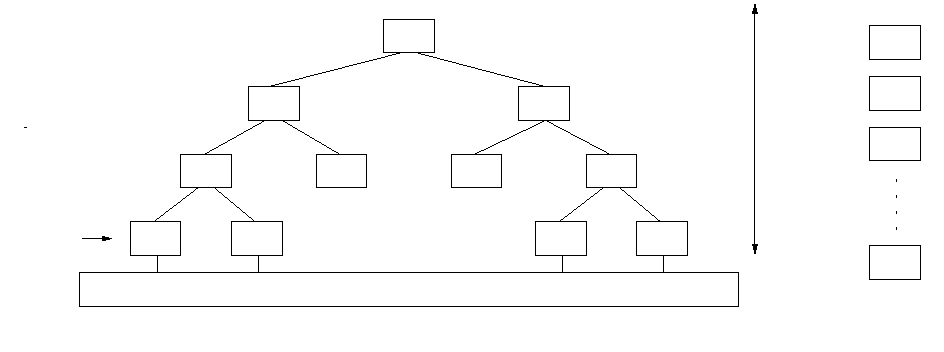
\includegraphics{Lecture35-Dinesh/figs/fig1.pdf}%
\end{picture}%
\setlength{\unitlength}{4144sp}%
%
\begingroup\makeatletter\ifx\SetFigFont\undefined%
\gdef\SetFigFont#1#2#3#4#5{%
  \reset@font\fontsize{#1}{#2pt}%
  \fontfamily{#3}\fontseries{#4}\fontshape{#5}%
  \selectfont}%
\fi\endgroup%
\begin{picture}(7191,2676)(3631,-7990)
\put(10183,-7942){\makebox(0,0)[lb]{\smash{{\SetFigFont{7}{8.4}{\rmdefault}{\mddefault}{\updefault}{\color[rgb]{0,0,0}computation}%
}}}}
\put(10183,-7796){\makebox(0,0)[lb]{\smash{{\SetFigFont{7}{8.4}{\rmdefault}{\mddefault}{\updefault}{\color[rgb]{0,0,0}Sequential}%
}}}}
\put(9463,-7539){\makebox(0,0)[lb]{\smash{{\SetFigFont{7}{8.4}{\rmdefault}{\mddefault}{\updefault}{\color[rgb]{0,0,0}Input}%
}}}}
\put(9463,-6304){\makebox(0,0)[lb]{\smash{{\SetFigFont{7}{8.4}{\rmdefault}{\mddefault}{\updefault}{\color[rgb]{0,0,0}depth}%
}}}}
\put(3646,-7153){\makebox(0,0)[lb]{\smash{{\SetFigFont{7}{8.4}{\rmdefault}{\mddefault}{\updefault}{\color[rgb]{0,0,0}Processors}%
}}}}
\put(5859,-7847){\makebox(0,0)[lb]{\smash{{\SetFigFont{7}{8.4}{\rmdefault}{\mddefault}{\updefault}{\color[rgb]{0,0,0}Parallel job computation}%
}}}}
\end{picture}%

\caption{Parallel and Sequential computation}
\label{figure1}
\end{figure}

But there can be parallelism in the outcomes of these processors. So we again
have a processors that receives the processed input and carry on the
processing (figure~\ref{figure1}) thereby leading levels of computation. 
In case of sequential computation, no such decomposition is possible : 
each processor in the same level will be executed one after the other and will 
be repeated for all the levels.

What would be the ``parallel'' time taken to finish the job ? This is nothing
but the time required to get the output. Since input to each level is
dependent on the output of the previous level, the delay caused will be
proportional to the length of the longest path.

Circuits essentially tries to abstract this idea.
\begin{definition}(Depth) Depth of any circuit $C$ is a function $\calD$ that
takes in circuit and gives the length of the longest path from root 
(output) to any leaf (input).
\end{definition}

\begin{definition}(Size) Size of a circuit $C$ is a function $\calS$ 
that takes a circuit and gives the number of gates (or devices) in the circuit.

Note that the size of a circuit can also be thought as the time taken by a
sequential machine to compute the same function.
\end{definition}

\begin{example}
Consider the parity function $f : \{0,1\}^n \to \{0,1\}$ where
$f(x_1,x_2,\ldots,x_n) = x_1 \oplus x_2 \oplus \ldots \oplus x_n$. The
circuit corresponding to this function is as shown in figure~\ref{figure2}.

\begin{figure}[htp!]
\centering
\begin{picture}(0,0)%
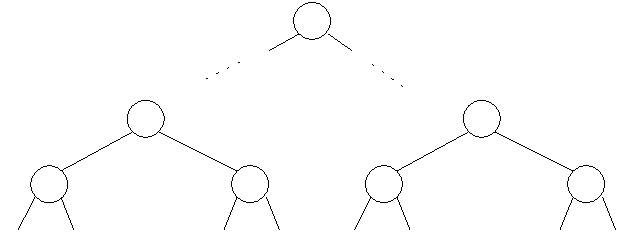
\includegraphics{Lecture35-Dinesh/figs/fig2.pdf}%
\end{picture}%
\setlength{\unitlength}{4144sp}%
%
\begingroup\makeatletter\ifx\SetFigFont\undefined%
\gdef\SetFigFont#1#2#3#4#5{%
  \reset@font\fontsize{#1}{#2pt}%
  \fontfamily{#3}\fontseries{#4}\fontshape{#5}%
  \selectfont}%
\fi\endgroup%
\begin{picture}(4702,1911)(886,-2197)
\put(5004,-2151){\makebox(0,0)[lb]{\smash{{\SetFigFont{7}{8.4}{\rmdefault}{\mddefault}{\updefault}{\color[rgb]{0,0,0}$x_{n-1}$}%
}}}}
\put(5452,-2151){\makebox(0,0)[lb]{\smash{{\SetFigFont{7}{8.4}{\rmdefault}{\mddefault}{\updefault}{\color[rgb]{0,0,0}$x_n$}%
}}}}
\put(1349,-2151){\makebox(0,0)[lb]{\smash{{\SetFigFont{7}{8.4}{\rmdefault}{\mddefault}{\updefault}{\color[rgb]{0,0,0}$x_2$}%
}}}}
\put(901,-2151){\makebox(0,0)[lb]{\smash{{\SetFigFont{7}{8.4}{\rmdefault}{\mddefault}{\updefault}{\color[rgb]{0,0,0}$x_1$}%
}}}}
\put(2443,-2151){\makebox(0,0)[lb]{\smash{{\SetFigFont{7}{8.4}{\rmdefault}{\mddefault}{\updefault}{\color[rgb]{0,0,0}$x_3$}%
}}}}
\put(2890,-2151){\makebox(0,0)[lb]{\smash{{\SetFigFont{7}{8.4}{\rmdefault}{\mddefault}{\updefault}{\color[rgb]{0,0,0}$x_4$}%
}}}}
\put(3164,-485){\makebox(0,0)[lb]{\smash{{\SetFigFont{7}{8.4}{\rmdefault}{\mddefault}{\updefault}{\color[rgb]{0,0,0}$+$}%
}}}}
\put(4457,-1231){\makebox(0,0)[lb]{\smash{{\SetFigFont{7}{8.4}{\rmdefault}{\mddefault}{\updefault}{\color[rgb]{0,0,0}$+$}%
}}}}
\put(5253,-1728){\makebox(0,0)[lb]{\smash{{\SetFigFont{7}{8.4}{\rmdefault}{\mddefault}{\updefault}{\color[rgb]{0,0,0}$+$}%
}}}}
\put(3711,-1728){\makebox(0,0)[lb]{\smash{{\SetFigFont{7}{8.4}{\rmdefault}{\mddefault}{\updefault}{\color[rgb]{0,0,0}$+$}%
}}}}
\put(2691,-1728){\makebox(0,0)[lb]{\smash{{\SetFigFont{7}{8.4}{\rmdefault}{\mddefault}{\updefault}{\color[rgb]{0,0,0}$+$}%
}}}}
\put(1896,-1231){\makebox(0,0)[lb]{\smash{{\SetFigFont{7}{8.4}{\rmdefault}{\mddefault}{\updefault}{\color[rgb]{0,0,0}$+$}%
}}}}
\put(1171,-1726){\makebox(0,0)[lb]{\smash{{\SetFigFont{7}{8.4}{\rmdefault}{\mddefault}{\updefault}{\color[rgb]{0,0,0}$+$}%
}}}}
\end{picture}%

\caption{The parity function}
\label{figure2}
\end{figure}
Note that we have exploited the associativity property of $\oplus$.
This circuit has a size $= n-1$ and depth $=\lceil\log_2 n \rceil$.
\end{example}

The next natural question to ask is 
\begin{center}
Will the parameters $\calS$ and $\calD$ depend on the complete basis chosen ?
\end{center}
The answer is yes and we now give a more accurate definition of size and
depth in terms of languages.
\begin{definition}Size $S_\Omega(L)$ of a language $L$ is the minimum
sized\footnote{By minimum sized, we mean asymptotic size i.e. constant
factors are ignored} function of a circuit family that computes $L$ for the
complete basis $\Omega$.
\end{definition}
\begin{definition}Depth $D_\Omega(L)$ of a language $L$ is the minimum
depth function of a circuit family that computes $L$ for the
complete basis $\Omega$.
\end{definition}

\begin{definition}Circuit Complexity of a language $L$ for a complete basis
$\Omega$ is defined as the tuple $(\calS_\Omega(L), \calD_\Omega(L))$ which
corresponds to the size and depth complexities respectively.
\end{definition}

\begin{claim}
\label{basis}
Let $\Omega$, $\Omega'$ be two finite complete basis of boolean functions of
fixed arity. Then for any $L \in \Sigma^*$,
\[ \calS_\Omega(L) = \Theta(\calS_{\Omega'}(L)), 
 \calD_\Omega(L) = \Theta(\calD_{\Omega'}(L)) \] 
\end{claim}
\begin{proof-idea}
Let $\{C_n\}_{n \ge 0}$ be the minimum sized circuit computing $L$ for the
complete basis $\Omega$. When the basis is changed, one need to express
boolean functions in $\Omega$ in terms of boolean functions in $\Omega'$.
This is always possible since $\Omega'$ is complete. Now a circuit in
the basis $\Omega'$ can be obtained by replacing the gates in $\Omega$ by
their equivalent circuits in $\Omega'$.

Note that the basis is finite and is independent of $n$. So the blow up or
shrinkage of each gate $C_n$ will only be by a constant. Hence in the worst
case all the gates in $\{C_n\}$ gets scaled by a constant factor and the size
of the resultant circuit can be at most $k \times$ size of original circuit. 
In case of depth, the length of the longest path gets scaled up (or down) by 
a factor independent of $n$.
\end{proof-idea}


Now we define the complexity class corresponding to the circuits computing a
function.
\begin{definition} For functions $f,g : \N \to \N$
\begin{align*}
SIZE(f(n)) & = \{ L | L \text{ is computed by a family of circuits of size }
f(n) \} \\
DEPTH(g(n)) & = \{ L | L \text{ is computed by a family of circuits of depth }
g(n) \} 
\end{align*}
\end{definition}

\section{Size of Circuits computing Boolean functions}
Consider a boolean function $f: \{0,1\}^n \to \{0,1\}$ defined on the
variables $(x_1,x_2,\ldots,x_n) \in \{0,1\}^n$ and the complete basis
$\Omega = \{\land,\lor,\neg\}$ where each function is having an arity $2$.
By claim~\ref{basis}, we have already seen that fixing the basis to be finite
gives us the guarantee that the same result holds in other bases
asymptotically. From now on we shall be working on this complete basis.

We would like to know what would be the size of the circuit computing $f$. How
large or small can it be ? Before answering them let us see what would be the
trivial circuit computing $f$.

An easy way to look at $f$ is to express it as sum-of-product terms (which can
be figured out from the truth table of $f$). Hence 
\[ f(x_1,x_2,\ldots,x_n) = \bigvee_{f(a_1,a_2,\ldots,a_n) = 1}(x_1^{a_1} \land
x_2^{a_2} \land \ldots \land x_n^{a_n} ) \]
where,
\[ x_i^{a_i} = \begin{cases}
		\overline{x_i} & \text{if } a_i = 0, \\
		x_i & \text{if } a_i = 1
		\end{cases} \]
\pagebreak

A circuit representation of $f$ (shown in figure~\ref{figure3})
\begin{figure}[htp!]
\centering
\begin{picture}(0,0)%
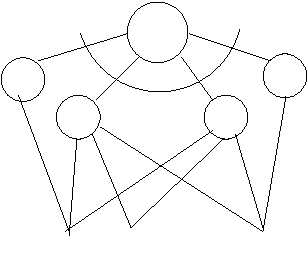
\includegraphics{Lecture35-Dinesh/figs/fig3.pdf}%
\end{picture}%
\setlength{\unitlength}{4144sp}%
%
\begingroup\makeatletter\ifx\SetFigFont\undefined%
\gdef\SetFigFont#1#2#3#4#5{%
  \reset@font\fontsize{#1}{#2pt}%
  \fontfamily{#3}\fontseries{#4}\fontshape{#5}%
  \selectfont}%
\fi\endgroup%
\begin{picture}(2347,1973)(3246,-3010)
\put(3624,-2912){\makebox(0,0)[lb]{\smash{{\SetFigFont{8}{9.6}{\familydefault}{\mddefault}{\updefault}{\color[rgb]{0,0,0}$x_1$}%
}}}}
\put(4097,-2912){\makebox(0,0)[lb]{\smash{{\SetFigFont{8}{9.6}{\familydefault}{\mddefault}{\updefault}{\color[rgb]{0,0,0}$x_2$}%
}}}}
\put(5100,-2912){\makebox(0,0)[lb]{\smash{{\SetFigFont{8}{9.6}{\familydefault}{\mddefault}{\updefault}{\color[rgb]{0,0,0}$x_n$}%
}}}}
\put(5130,-1228){\makebox(0,0)[lb]{\smash{{\SetFigFont{8}{9.6}{\rmdefault}{\mddefault}{\updefault}{\color[rgb]{0,0,0}$2^n$}%
}}}}
\put(3376,-1681){\makebox(0,0)[lb]{\smash{{\SetFigFont{8}{9.6}{\familydefault}{\mddefault}{\updefault}{\color[rgb]{0,0,0}$\land$}%
}}}}
\put(3826,-1951){\makebox(0,0)[lb]{\smash{{\SetFigFont{8}{9.6}{\familydefault}{\mddefault}{\updefault}{\color[rgb]{0,0,0}$\land$}%
}}}}
\put(4951,-1951){\makebox(0,0)[lb]{\smash{{\SetFigFont{8}{9.6}{\familydefault}{\mddefault}{\updefault}{\color[rgb]{0,0,0}$\land$}%
}}}}
\put(5401,-1636){\makebox(0,0)[lb]{\smash{{\SetFigFont{8}{9.6}{\familydefault}{\mddefault}{\updefault}{\color[rgb]{0,0,0}$\land$}%
}}}}
\put(4411,-1321){\makebox(0,0)[lb]{\smash{{\SetFigFont{12}{14.4}{\familydefault}{\mddefault}{\updefault}{\color[rgb]{0,0,0}$\vee$}%
}}}}
\put(4366,-2041){\makebox(0,0)[lb]{\smash{{\SetFigFont{12}{14.4}{\rmdefault}{\mddefault}{\updefault}{\color[rgb]{0,0,0}$\ldots$}%
}}}}
\put(4546,-2941){\makebox(0,0)[lb]{\smash{{\SetFigFont{12}{14.4}{\rmdefault}{\mddefault}{\updefault}{\color[rgb]{0,0,0}$\ldots$}%
}}}}
\end{picture}%

\caption{Circuit representation of $f$}
\label{figure3}
\end{figure}
has a root $\vee$ gate with $2^n$ inputs. But our basis has $\lor$ gates of 
arity $2$. Reduction to arity $2$ can be achieved by composing $\lor$ as shown.
in figure~\ref{figure4}
\begin{figure}[htp!]
\centering
\begin{picture}(0,0)%
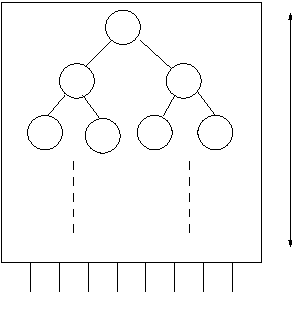
\includegraphics{Lecture35-Dinesh/figs/fig4.pdf}%
\end{picture}%
\setlength{\unitlength}{4144sp}%
%
\begingroup\makeatletter\ifx\SetFigFont\undefined%
\gdef\SetFigFont#1#2#3#4#5{%
  \reset@font\fontsize{#1}{#2pt}%
  \fontfamily{#3}\fontseries{#4}\fontshape{#5}%
  \selectfont}%
\fi\endgroup%
\begin{picture}(2271,2451)(1789,-3175)
\put(4045,-1638){\makebox(0,0)[lb]{\smash{{\SetFigFont{5}{6.0}{\rmdefault}{\mddefault}{\updefault}{\color[rgb]{0,0,0}depth $n$}%
}}}}
\put(3408,-1749){\makebox(0,0)[lb]{\smash{{\SetFigFont{5}{6.0}{\rmdefault}{\mddefault}{\updefault}{\color[rgb]{0,0,0}$\lor$}%
}}}}
\put(3166,-1352){\makebox(0,0)[lb]{\smash{{\SetFigFont{5}{6.0}{\rmdefault}{\mddefault}{\updefault}{\color[rgb]{0,0,0}$\lor$}%
}}}}
\put(2725,-957){\makebox(0,0)[lb]{\smash{{\SetFigFont{5}{6.0}{\rmdefault}{\mddefault}{\updefault}{\color[rgb]{0,0,0}$\lor$}%
}}}}
\put(2351,-1352){\makebox(0,0)[lb]{\smash{{\SetFigFont{5}{6.0}{\rmdefault}{\mddefault}{\updefault}{\color[rgb]{0,0,0}$\lor$}%
}}}}
\put(2548,-1771){\makebox(0,0)[lb]{\smash{{\SetFigFont{5}{6.0}{\rmdefault}{\mddefault}{\updefault}{\color[rgb]{0,0,0}$\lor$}%
}}}}
\put(2637,-3136){\makebox(0,0)[lb]{\smash{{\SetFigFont{5}{6.0}{\rmdefault}{\mddefault}{\updefault}{\color[rgb]{0,0,0}$2^n$ inputs}%
}}}}
\put(2109,-1749){\makebox(0,0)[lb]{\smash{{\SetFigFont{5}{6.0}{\rmdefault}{\mddefault}{\updefault}{\color[rgb]{0,0,0}$\lor$}%
}}}}
\put(2945,-1749){\makebox(0,0)[lb]{\smash{{\SetFigFont{5}{6.0}{\rmdefault}{\mddefault}{\updefault}{\color[rgb]{0,0,0}$\lor$}%
}}}}
\end{picture}%

\caption{Arity reduction of root $\lor$ gate}
\label{figure4}
\end{figure}
and replacing the root $\lor$ gate in figure~\ref{figure3} by this circuit. 
Again the $\land$ gates are taking $n$ inputs: hence we replace the $\land$ 
gate by composing $\land$ s as shown in figure~\ref{figure5} 
and plug it in place of $\land$ in figure~\ref{figure3}.

\begin{figure}[htp!]
\centering
\begin{picture}(0,0)%
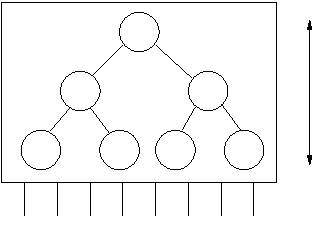
\includegraphics{Lecture35-Dinesh/figs/fig5.pdf}%
\end{picture}%
\setlength{\unitlength}{4144sp}%
%
\begingroup\makeatletter\ifx\SetFigFont\undefined%
\gdef\SetFigFont#1#2#3#4#5{%
  \reset@font\fontsize{#1}{#2pt}%
  \fontfamily{#3}\fontseries{#4}\fontshape{#5}%
  \selectfont}%
\fi\endgroup%
\begin{picture}(2401,1837)(1834,-2561)
\put(2021,-1886){\makebox(0,0)[lb]{\smash{{\SetFigFont{7}{8.4}{\familydefault}{\mddefault}{\updefault}{\color[rgb]{0,0,0}$\land$}%
}}}}
\put(2321,-1436){\makebox(0,0)[lb]{\smash{{\SetFigFont{7}{8.4}{\rmdefault}{\mddefault}{\updefault}{\color[rgb]{0,0,0}$\land$}%
}}}}
\put(2621,-1886){\makebox(0,0)[lb]{\smash{{\SetFigFont{7}{8.4}{\familydefault}{\mddefault}{\updefault}{\color[rgb]{0,0,0}$\land$}%
}}}}
\put(3046,-1886){\makebox(0,0)[lb]{\smash{{\SetFigFont{7}{8.4}{\familydefault}{\mddefault}{\updefault}{\color[rgb]{0,0,0}$\land$}%
}}}}
\put(3296,-1436){\makebox(0,0)[lb]{\smash{{\SetFigFont{7}{8.4}{\familydefault}{\mddefault}{\updefault}{\color[rgb]{0,0,0}$\land$}%
}}}}
\put(2771,-986){\makebox(0,0)[lb]{\smash{{\SetFigFont{7}{8.4}{\familydefault}{\mddefault}{\updefault}{\color[rgb]{0,0,0}$\land$}%
}}}}
\put(3571,-1886){\makebox(0,0)[lb]{\smash{{\SetFigFont{7}{8.4}{\familydefault}{\mddefault}{\updefault}{\color[rgb]{0,0,0}$\land$}%
}}}}
\put(2671,-2511){\makebox(0,0)[lb]{\smash{{\SetFigFont{7}{8.4}{\familydefault}{\mddefault}{\updefault}{\color[rgb]{0,0,0}$n$ inputs}%
}}}}
\put(4220,-1486){\makebox(0,0)[lb]{\smash{{\SetFigFont{7}{8.4}{\familydefault}{\mddefault}{\updefault}{\color[rgb]{0,0,0}depth $\lceil \log n \rceil$}%
}}}}
\end{picture}%

\caption{Arity reduction of $\land$ gate}
\label{figure5}
\end{figure}

Now size of the circuit 
\begin{align*}
= &   (2^{n+1}-1)  && \text{[due to $\lor$ gates]} \\ 
  & + 2^n \times (2n-1) && \text{[due to $2^n$ $\land$ 
  gates each of size $(2n-1)$]} \\
  =&  O(n 2^n) 
\end{align*}

A takeaway from the whole exercise is that any function $f$ on $n$ input can
be represented using a circuit of size $O(n2^n)$.
A natural question is : can there be circuits of even smaller size ?

We shall now see a lower bound due to Shannon(1942) and an upper bound due to
Lupanov(1952) on the size of a boolean circuit computing a function $f$.

\section{Shannon's Lower bound}
\begin{theorem}(Shannon, 1942) For  ``most'' of the circuits on $n$ inputs
computing a function $f$, the size of the circuit is larger than
$\frac{2^n}{n}$ (asymptotically)
\end{theorem}
\begin{proof}
Proof is by a counting argument on the number of boolean circuits on $n$
inputs and of size $s$ computing $f$. We argue that if we restrict the size of
the circuit $s < \frac{2^n}{n}$, then the fraction of functions that can be
computed using such circuits is very small.

Let $H(n,s)$ be the number of distinct circuits possible on $n$ inputs and of
size $s$. Observe that $s \ge n$. Since the circuit is characterised by a
(unique) root, $s-1$ gates and $n$ inputs, we count how many ways can the $s$
gates be \emph{selected}. The count can be split as,
\begin{itemize}
\item No. of ways of fixing the root $\to$ $s$ ways.
\item Each of the internal gates (gates other than the root)
   \begin{itemize}
   \item can compute $2^{2^2}$ functions\footnote{$\neg$ can be assumed to be
   of two input where it negates one input and ignores the other.}
   \item there are $(n+s)$ possible inputs for each function and hence $(n+s)^2$
   possible choices.
   \end{itemize}
\item Hence total ways is $s[16(n+s)^2]^{s-1}$.
\end{itemize}

But each permutation of the gates is going to give us the same circuit. Hence
total number of distinct circuits is bounded by
\[ H(n,s) \le  \frac{s[16(n+s)^2]^{s-1}}{s!} \]
(Note that we are only looking locally at what is the requirement of each gate.
Circuits are DAGs but since the choices made at each gate is local, we can
have cycles. Hence we are counting the non-DAG circuits also. But still this
count remains an upper bound)

Now, 
\[ \log H(n,s) \le \log s + (s-1)\log [16(n+s)^2] - \log s! \]
By Stirling approximation, $s! \ge \left ( \frac{s}{e} \right )^s$, we have
$\log s! \ge s\log s- s\log e$
\begin{align*}
\log H(n,s) & \le \log s + (s-1)\log[16(n+s)^2] - (s\log s -s \log e) \\
 & = \log s + 2(s-1) \log (n+s) + (s-1) \log 16 -(s\log s -s\log s) \\
\end{align*}
Now, since $n \le s$ we have $n+s \le 2s$.
\begin{align*}
\log H(n,s) & \le \log s + 2(s-1)\log 2s + (s-1)\log 16 - (s\log s - s\log e)
\\
& < \log s + 2s\log (2s) + s \log 16 + s\log e \\
& = (1+s)\log s + 6s + s\log e
\end{align*}
Substituting $s = \frac{2^n}{n}$, we get,
\begin{align*}
\log H(n,s) & <  \left ( \frac{2^n}{n}+1 \right ) (n-\log n) + (6 + \log e)
\frac{2^n}{n} \\
& = 2^n -\frac{2^n}{n}[\log n - (6 + \log e)] + n - \log n \\
& = 2^n - \frac{2^n}{n} \left [ \log n - (6+\log e) - \frac{n}{2^n}(n-\log n) 
\right ] \\
& = 2^n -\frac{2^n}{n} \log n \left [ 1 - \frac{(6+\log e)}{\log n} -
\frac{n(n-\log n)}{2^n\log n}  \right ] \\
& = 2^n - \frac{2^n}{n} \log n [1 - o(1)]
\end{align*}
Hence asymptotically,
\[ H\left (n, \frac{2^n}{n}\right ) \le \frac{2^{2^n}}{2^{\frac{2^n}{n} \log n (1 - o(1))}}
\]
Since $2^{2^n}$ is the total number of functions on $n$ inputs, we have,
\[ H\left (n,\frac{2^n}{n}\right  ) = 2^{-\frac{2^n}{n} \log n
(1-o(1))}(\text{Total no. of functions on input } n) \]
Hence the fraction of functions that can be computed with small size is very
less since the number of distinct circuits is an exponentially small fraction
of total functions on $n$ inputs. Hence we conclude that large fraction of
functions require size $ > \frac{2^n}{n}$.
\end{proof}

\section{Lupanov's Upper bound}
Shannon's lower bound says that there is (asymptotically) large fraction 
of functions that remains uncomputable with circuits of size 
$ < \frac{2^n}{n}$. What Lupanov's bound says is, if we allow circuit size to
be larger by a small fraction of $\frac{2^n}{n}$, then we can compute
all functions in $n$ inputs.

Let $f:\{0,1\}^n \to \{0,1\}$ be a boolean function. We can express
$f(x_1,x_2,\ldots,x_n)$ as \[(x_1\land f(1,x_2,\ldots,x_n)) \lor 
(\overline{x_1}\land f(0,x_2,\ldots,x_n))\] 

\begin{figure}[htp!]
\centering
\begin{picture}(0,0)%
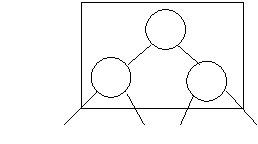
\includegraphics{Lecture35-Dinesh/figs/fig6.pdf}%
\end{picture}%
\setlength{\unitlength}{4144sp}%
%
\begingroup\makeatletter\ifx\SetFigFont\undefined%
\gdef\SetFigFont#1#2#3#4#5{%
  \reset@font\fontsize{#1}{#2pt}%
  \fontfamily{#3}\fontseries{#4}\fontshape{#5}%
  \selectfont}%
\fi\endgroup%
\begin{picture}(1968,1093)(2146,-2402)
\put(2161,-2311){\makebox(0,0)[lb]{\smash{{\SetFigFont{7}{8.4}{\familydefault}{\mddefault}{\updefault}{\color[rgb]{0,0,0}$f(1,x_2,\ldots,x_n)$}%
}}}}
\put(3466,-2356){\makebox(0,0)[lb]{\smash{{\SetFigFont{7}{8.4}{\familydefault}{\mddefault}{\updefault}{\color[rgb]{0,0,0}$\overline{x_1}$}%
}}}}
\put(3151,-2356){\makebox(0,0)[lb]{\smash{{\SetFigFont{7}{8.4}{\familydefault}{\mddefault}{\updefault}{\color[rgb]{0,0,0}$x_1$}%
}}}}
\put(3826,-2311){\makebox(0,0)[lb]{\smash{{\SetFigFont{7}{8.4}{\familydefault}{\mddefault}{\updefault}{\color[rgb]{0,0,0}$f(0,x_2,\ldots,x_n)$}%
}}}}
\put(3376,-1591){\makebox(0,0)[lb]{\smash{{\SetFigFont{7}{8.4}{\familydefault}{\mddefault}{\updefault}{\color[rgb]{0,0,0}$\lor$}%
}}}}
\put(3736,-1951){\makebox(0,0)[lb]{\smash{{\SetFigFont{7}{8.4}{\familydefault}{\mddefault}{\updefault}{\color[rgb]{0,0,0}$\lor$}%
}}}}
\put(2971,-1951){\makebox(0,0)[lb]{\smash{{\SetFigFont{7}{8.4}{\familydefault}{\mddefault}{\updefault}{\color[rgb]{0,0,0}$\lor$}%
}}}}
\end{picture}%

\caption{Circuit computing $f$}
\label{figure6}
\end{figure}
Hence $f(x_1,x_2,\ldots,x_n)$ can be expressed in the form of a recursive 
structure as, 
\begin{figure}[htp!]
\centering
\begin{picture}(0,0)%
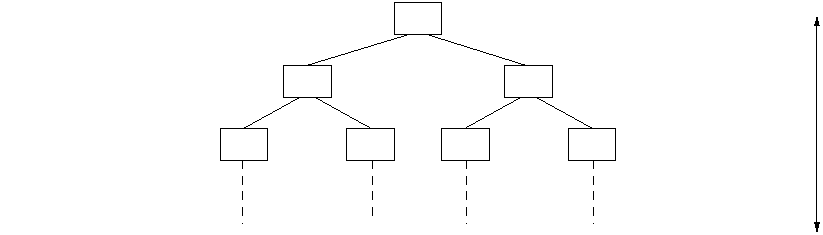
\includegraphics{Lecture35-Dinesh/figs/fig7.pdf}%
\end{picture}%
\setlength{\unitlength}{4144sp}%
%
\begingroup\makeatletter\ifx\SetFigFont\undefined%
\gdef\SetFigFont#1#2#3#4#5{%
  \reset@font\fontsize{#1}{#2pt}%
  \fontfamily{#3}\fontseries{#4}\fontshape{#5}%
  \selectfont}%
\fi\endgroup%
\begin{picture}(6266,1782)(-239,-2956)
\put(6012,-2029){\makebox(0,0)[lb]{\smash{{\SetFigFont{7}{8.4}{\familydefault}{\mddefault}{\updefault}{\color[rgb]{0,0,0}$n$}%
}}}}
\put(1971,-1836){\makebox(0,0)[lb]{\smash{{\SetFigFont{7}{8.4}{\familydefault}{\mddefault}{\updefault}{\color[rgb]{0,0,0}$x_2$}%
}}}}
\put(3657,-1836){\makebox(0,0)[lb]{\smash{{\SetFigFont{7}{8.4}{\familydefault}{\mddefault}{\updefault}{\color[rgb]{0,0,0}$x_2$}%
}}}}
\put(4138,-2317){\makebox(0,0)[lb]{\smash{{\SetFigFont{7}{8.4}{\familydefault}{\mddefault}{\updefault}{\color[rgb]{0,0,0}$x_3$}%
}}}}
\put(3175,-2317){\makebox(0,0)[lb]{\smash{{\SetFigFont{7}{8.4}{\familydefault}{\mddefault}{\updefault}{\color[rgb]{0,0,0}$x_3$}%
}}}}
\put(2453,-2317){\makebox(0,0)[lb]{\smash{{\SetFigFont{7}{8.4}{\familydefault}{\mddefault}{\updefault}{\color[rgb]{0,0,0}$x_3$}%
}}}}
\put(2815,-1354){\makebox(0,0)[lb]{\smash{{\SetFigFont{7}{8.4}{\familydefault}{\mddefault}{\updefault}{\color[rgb]{0,0,0}$x_1$}%
}}}}
\put(3271,-1354){\makebox(0,0)[lb]{\smash{{\SetFigFont{7}{8.4}{\familydefault}{\mddefault}{\updefault}{\color[rgb]{0,0,0}Computes $f(x_1,x_2,\ldots,x_n)$}%
}}}}
\put(4090,-1764){\makebox(0,0)[lb]{\smash{{\SetFigFont{7}{8.4}{\familydefault}{\mddefault}{\updefault}{\color[rgb]{0,0,0}Computes $f(1,x_2,\ldots,x_n)$}%
}}}}
\put(3513,-1546){\makebox(0,0)[lb]{\smash{{\SetFigFont{7}{8.4}{\familydefault}{\mddefault}{\updefault}{\color[rgb]{0,0,0}$x_1=1$}%
}}}}
\put(2044,-1546){\makebox(0,0)[lb]{\smash{{\SetFigFont{7}{8.4}{\familydefault}{\mddefault}{\updefault}{\color[rgb]{0,0,0}$x_1=0$}%
}}}}
\put(1490,-2317){\makebox(0,0)[lb]{\smash{{\SetFigFont{7}{8.4}{\familydefault}{\mddefault}{\updefault}{\color[rgb]{0,0,0}$x_3$}%
}}}}
\put(4478,-2311){\makebox(0,0)[lb]{\smash{{\SetFigFont{7}{8.4}{\familydefault}{\mddefault}{\updefault}{\color[rgb]{0,0,0}Computes $f(1,1,\ldots,x_n)$}%
}}}}
\put(-224,-2311){\makebox(0,0)[lb]{\smash{{\SetFigFont{7}{8.4}{\familydefault}{\mddefault}{\updefault}{\color[rgb]{0,0,0}Computes $f(0,0,x_3\ldots,x_n)$}%
}}}}
\put(316,-1861){\makebox(0,0)[lb]{\smash{{\SetFigFont{7}{8.4}{\familydefault}{\mddefault}{\updefault}{\color[rgb]{0,0,0}Computes $f(0,x_2,\ldots,x_n)$}%
}}}}
\end{picture}%

\caption{Complete circuit computing $f$}
\label{figure7}
\end{figure}
where each box represents the two $\land$ and one $\lor$ of 
figure~\ref{figure6}. 
Now, we can find the size of the circuit follows the recurrence 
\[S(n) =2S(n-1) + 6\]\[ S(2) = 1 \] where $6 = (1 - \land, 2 - \lor, 
\text{one } \neg \text{ of } \overline{x_1}, 
\text{ and } 0,1 \text{ inputs})$. Hence $S(n) = \frac{7}{4}2^n - 6 = O(2^n)$.
Note that this is a better bound than the bound from the trivial circuit. 
So the question is how much more can we improve ? How to make the circuit more 
compact ?
\begin{theorem}(Lupanov, 1952) An function on input defined on the complete
basis $\Omega = \{ \neg, \lor, \land\}$ of two input gates can be computed by a
 circuit of size $[1+o(1)]\frac{2^n}{n}$.
\end{theorem}
\begin{proof}
Observe that at the $k^{th}$ level (see figure~\ref{figure8}) for $0 < k \le n$ 
(where the bottom of the circuit is level 0) there are $k$ variables appearing
below it (All the $n-k$ variables above the $k^{th}$ level would have got
$0$ or $1$ assigned).
\begin{figure}[htp!]
\centering
\begin{picture}(0,0)%
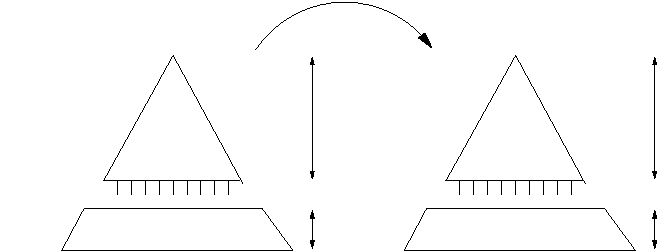
\includegraphics{Lecture35-Dinesh/figs/fig8.pdf}%
\end{picture}%
\setlength{\unitlength}{4144sp}%
%
\begingroup\makeatletter\ifx\SetFigFont\undefined%
\gdef\SetFigFont#1#2#3#4#5{%
  \reset@font\fontsize{#1}{#2pt}%
  \fontfamily{#3}\fontseries{#4}\fontshape{#5}%
  \selectfont}%
\fi\endgroup%
\begin{picture}(5068,1913)(2146,-2683)
\put(7178,-1716){\makebox(0,0)[lb]{\smash{{\SetFigFont{6}{7.2}{\familydefault}{\mddefault}{\updefault}{\color[rgb]{0,0,0}$n-k$}%
}}}}
\put(7199,-2501){\makebox(0,0)[lb]{\smash{{\SetFigFont{6}{7.2}{\familydefault}{\mddefault}{\updefault}{\color[rgb]{0,0,0}$k$}%
}}}}
\put(4568,-1716){\makebox(0,0)[lb]{\smash{{\SetFigFont{6}{7.2}{\familydefault}{\mddefault}{\updefault}{\color[rgb]{0,0,0}$n-k$}%
}}}}
\put(4590,-2501){\makebox(0,0)[lb]{\smash{{\SetFigFont{6}{7.2}{\familydefault}{\mddefault}{\updefault}{\color[rgb]{0,0,0}$k$}%
}}}}
\put(2999,-2565){\makebox(0,0)[lb]{\smash{{\SetFigFont{6}{7.2}{\familydefault}{\mddefault}{\updefault}{\color[rgb]{0,0,0}Dependent on $k$ inputs}%
}}}}
\put(2161,-2086){\makebox(0,0)[lb]{\smash{{\SetFigFont{6}{7.2}{\familydefault}{\mddefault}{\updefault}{\color[rgb]{0,0,0}$3.2^{n-k}$ gates}%
}}}}
\put(5851,-2446){\makebox(0,0)[lb]{\smash{{\SetFigFont{6}{7.2}{\familydefault}{\mddefault}{\updefault}{\color[rgb]{0,0,0}$A(k)$ gates }%
}}}}
\put(5626,-2626){\makebox(0,0)[lb]{\smash{{\SetFigFont{6}{7.2}{\familydefault}{\mddefault}{\updefault}{\color[rgb]{0,0,0}(All $2^{2^k}$ functions)}%
}}}}
\end{picture}%

\caption{Compacting of circuit}
\label{figure8}
\end{figure}

Also from our construction, it is clear that there are $3(2^{n-k})$ gates at
the $k^{th}$ level. Since circuits are DAGs the input to these gates can only
come from the $k$ variables. Also there can be $2^{2^k}$ distinct functions
computable using $k$ inputs. Now if $A(k)$ is the number of gates required to
realise these $2^{2^k}$ distinct functions then the $3(2^{n-k})$ gates can get
input from any of the $A(k)$ gates and if we have the case where $3(2^{n-k}) >
A(k)$ (after appropriately setting $k$), the result of computation can be
reused and compaction can be achieved. So unlike the earlier case where we
might have needed at least $3(2^{n-k})$ gates below the $k^{th}$ level, it now
suffices to generate all $2^{2^k}$ functions.

Now it remains to estimate $A(k)$. This function can be recursively
characterised as \[(x_k \land f_1(x_1,x_2,\ldots,x_{k-1}) \lor (\overline{x_k}
\land f_2(x_1,x_2,\ldots,x_{k-1})\] If we have the circuits computing all 
the $k-1$ input functions, we can construct circuits computing 
all of the $k$ input function using the recursive formulation.

Note that the total number of gates required to realise $2^{2^k}$ functions =
$ A(k) $ 
\begin{center} = (Gates required to realise $k$ variate functions from circuit
computing functions on $k-1$ variables) 

$+$ 

Number of gates required to realise all the $2^{2^{k-1}}$ functions.
\end{center}

The first term equals
\begin{align*}
= & \text{Total no. of $\land$ gates} + \text{Total no. of $\lor$ gates}  \\
= & (2^{2^{k-1}}) \times 2 +  (2^{2^{k-1}}) \times (2^{2^{k-1}}) 
&& [\text{Two $\land$ gates per $f$}] \\
& && [\text{Ways of choosing $f_1$, $f_2$}] 
\end{align*}
The second term is nothing but $A(k-1)$. Hence,
\begin{align*}
A(k) &=  A(k-1) + 2^{2^{k-1}} \times 2 + 2^{2^k} \\
A(0) &= 2 &&[\text{i.e. True or False}] 
\end{align*}
Note that this is nothing but the series summation
\begin{align*}
= & \sum_{i=1}^k (2^{2^i} + 2.2^{2^{i-1}}) + A(0) \\
= & \sum_{i=1}^k 2^{2^i} + \sum_{i=1}^k 2.2^{2^{i-1}} + A(0) \\
= & \sum_{i=0}^{k-1} 2^{2^i} + \sum_{i=0}^{k-1} 2.2^{2^i} + 2 + 2^{2^k} + A(0)
\\
= & 3\sum_{i=0}^{k-1} 2^{2^i} + 4 + 2^{2^k} \\
< &~3\sum_{i=0}^{k-1} 2^{2^{k-1}} + 2^{2^k} \\
= & 2^{2^k}+ 3k.2^{2^{k-1}} = 2^{2^k} \left ( 1 + \frac{3k}{2^{({2^k} -
2^{k-1})}}  \right )\\
\end{align*}
Hence $A(k) =  2^{2^k}(1+ o(1))$. Therefore total number of gates = $3.2^{n-k}
+ 2^{2^k}(1+o(1))$. Now to have $3.2^{n-k} > 2^{2^k}$, we choose $k = \log (n
- \log n)$ (verification of $k$ is left to the reader). 
Total number of gates is now
\begin{align*}
= & 3.\frac{2^n}{n-\log n} + \frac{2^n}{n}(1+o(1)) \\
= & \frac{2^n}{n} \left [ \frac{3}{1-\frac{\log n}{n}} + 1 + o(1)\right ] \\
\le & \frac{2^n}{n}(4 + o(1))
\end{align*}
This proves a bound which is almost as tight as the Lupanov's bound. Reducing
the constant from $4$ to $1$ requires more effort.
\end{proof}




\bibliographystyle{abbrv}
\bibliography{references}

\end{document}
